\documentclass[twoside]{book}

% Packages required by doxygen
\usepackage{calc}
\usepackage{doxygen}
\usepackage{graphicx}
\usepackage[utf8]{inputenc}
\usepackage{makeidx}
\usepackage{multicol}
\usepackage{multirow}
\usepackage{textcomp}
\usepackage[table]{xcolor}

% Font selection
\usepackage[T1]{fontenc}
\usepackage{mathptmx}
\usepackage[scaled=.90]{helvet}
\usepackage{courier}
\usepackage{amssymb}
\usepackage{sectsty}
\renewcommand{\familydefault}{\sfdefault}
\allsectionsfont{%
  \fontseries{bc}\selectfont%
  \color{darkgray}%
}
\renewcommand{\DoxyLabelFont}{%
  \fontseries{bc}\selectfont%
  \color{darkgray}%
}

% Page & text layout
\usepackage{geometry}
\geometry{%
  a4paper,%
  top=2.5cm,%
  bottom=2.5cm,%
  left=2.5cm,%
  right=2.5cm%
}
\tolerance=750
\hfuzz=15pt
\hbadness=750
\setlength{\emergencystretch}{15pt}
\setlength{\parindent}{0cm}
\setlength{\parskip}{0.2cm}
\makeatletter
\renewcommand{\paragraph}{%
  \@startsection{paragraph}{4}{0ex}{-1.0ex}{1.0ex}{%
    \normalfont\normalsize\bfseries\SS@parafont%
  }%
}
\renewcommand{\subparagraph}{%
  \@startsection{subparagraph}{5}{0ex}{-1.0ex}{1.0ex}{%
    \normalfont\normalsize\bfseries\SS@subparafont%
  }%
}
\makeatother

% Headers & footers
\usepackage{fancyhdr}
\pagestyle{fancyplain}
\fancyhead[LE]{\fancyplain{}{\bfseries\thepage}}
\fancyhead[CE]{\fancyplain{}{}}
\fancyhead[RE]{\fancyplain{}{\bfseries\leftmark}}
\fancyhead[LO]{\fancyplain{}{\bfseries\rightmark}}
\fancyhead[CO]{\fancyplain{}{}}
\fancyhead[RO]{\fancyplain{}{\bfseries\thepage}}
\fancyfoot[LE]{\fancyplain{}{}}
\fancyfoot[CE]{\fancyplain{}{}}
\fancyfoot[RE]{\fancyplain{}{\bfseries\scriptsize Generated on Tue Jan 21 2014 12:32:13 for My Project by Doxygen }}
\fancyfoot[LO]{\fancyplain{}{\bfseries\scriptsize Generated on Tue Jan 21 2014 12:32:13 for My Project by Doxygen }}
\fancyfoot[CO]{\fancyplain{}{}}
\fancyfoot[RO]{\fancyplain{}{}}
\renewcommand{\footrulewidth}{0.4pt}
\renewcommand{\chaptermark}[1]{%
  \markboth{#1}{}%
}
\renewcommand{\sectionmark}[1]{%
  \markright{\thesection\ #1}%
}

% Indices & bibliography
\usepackage{natbib}
\usepackage[titles]{tocloft}
\setcounter{tocdepth}{3}
\setcounter{secnumdepth}{5}
\makeindex

% Hyperlinks (required, but should be loaded last)
\usepackage{ifpdf}
\ifpdf
  \usepackage[pdftex,pagebackref=true]{hyperref}
\else
  \usepackage[ps2pdf,pagebackref=true]{hyperref}
\fi
\hypersetup{%
  colorlinks=true,%
  linkcolor=blue,%
  citecolor=blue,%
  unicode%
}

% Custom commands
\newcommand{\clearemptydoublepage}{%
  \newpage{\pagestyle{empty}\cleardoublepage}%
}


%===== C O N T E N T S =====

\begin{document}

% Titlepage & ToC
\hypersetup{pageanchor=false}
\pagenumbering{roman}
\begin{titlepage}
\vspace*{7cm}
\begin{center}%
{\Large My Project }\\
\vspace*{1cm}
{\large Generated by Doxygen 1.8.4}\\
\vspace*{0.5cm}
{\small Tue Jan 21 2014 12:32:13}\\
\end{center}
\end{titlepage}
\clearemptydoublepage
\tableofcontents
\clearemptydoublepage
\pagenumbering{arabic}
\hypersetup{pageanchor=true}

%--- Begin generated contents ---
\chapter{Working with Road\-Runner Plugins}
\label{index}\hypertarget{index}{}\hypertarget{index_Introduction}{}\section{Introduction}\label{index_Introduction}

\begin{DoxyCode}
1 \textcolor{keywordflow}{print} \textcolor{stringliteral}{"Starting Test"}
2 input telplugins \textcolor{keyword}{as} *
3 p = Plugin (\textcolor{stringliteral}{"tel\_add\_noise"})
4 p.viewManual()
5 pl = p.listOfProperties()
6 \textcolor{keywordflow}{for} item \textcolor{keywordflow}{in} pl:
7     \textcolor{keywordflow}{print} item
8 
9 p.Sigma = 0.00005
10 series = DataSeries.loadDataSeries (\textcolor{stringliteral}{"..\(\backslash\)\(\backslash\)Examples\(\backslash\)\(\backslash\)testData.dat"})
11 series.plot()
12 p.InputData = series
13 p.execute()
14 p.InputData.plot()
15 
16 \textcolor{keywordflow}{print} \textcolor{stringliteral}{"Test Finished"}
\end{DoxyCode}
 
\chapter{Module Index}
\section{Modules}
Here is a list of all modules\-:\begin{DoxyCompactList}
\item \contentsline{section}{Plugin Manager}{\pageref{group__plugin__manager}}{}
\item \contentsline{section}{Plugin Functions}{\pageref{group__plugins}}{}
\item \contentsline{section}{Plugin Properties}{\pageref{group__plugin__properties}}{}
\item \contentsline{section}{Utility Functions}{\pageref{group__utilities}}{}
\end{DoxyCompactList}

\chapter{Hierarchical Index}
\section{Class Hierarchy}
This inheritance list is sorted roughly, but not completely, alphabetically\-:\begin{DoxyCompactList}
\item object\begin{DoxyCompactList}
\item \contentsline{section}{python.\-telplugins.\-Data\-Series}{\pageref{classpython_1_1telplugins_1_1_data_series}}{}
\item \contentsline{section}{python.\-telplugins.\-Event}{\pageref{classpython_1_1telplugins_1_1_event}}{}
\item \contentsline{section}{python.\-telplugins.\-Plugin}{\pageref{classpython_1_1telplugins_1_1_plugin}}{}
\end{DoxyCompactList}
\end{DoxyCompactList}

\chapter{Class Index}
\section{Class List}
Here are the classes, structs, unions and interfaces with brief descriptions\-:\begin{DoxyCompactList}
\item\contentsline{section}{\hyperlink{classpython_1_1telplugins_1_1_data_series}{python.\-telplugins.\-Data\-Series} \\*\hyperlink{classpython_1_1telplugins_1_1_data_series}{Data\-Series} class for handling roadrunner data types }{\pageref{classpython_1_1telplugins_1_1_data_series}}{}
\item\contentsline{section}{\hyperlink{classpython_1_1telplugins_1_1_event}{python.\-telplugins.\-Event} }{\pageref{classpython_1_1telplugins_1_1_event}}{}
\item\contentsline{section}{\hyperlink{classpython_1_1telplugins_1_1_plugin}{python.\-telplugins.\-Plugin} }{\pageref{classpython_1_1telplugins_1_1_plugin}}{}
\end{DoxyCompactList}

\chapter{Module Documentation}
\hypertarget{group__plugin__manager}{\section{Plugin Manager}
\label{group__plugin__manager}\index{Plugin Manager@{Plugin Manager}}
}


Plugin Manager Library Functions The Plugin manager loads and manages one or more plugins.  


\subsection*{Functions}
\begin{DoxyCompactItemize}
\item 
def \hyperlink{group__plugin__manager_ga20d1fd0f6e3a77a1b80a2d32911cf2a5}{python.\-telplugins\-\_\-c\-\_\-api.\-create\-Plugin\-Manager}
\begin{DoxyCompactList}\small\item\em Create a new instance of a plugin manager. \end{DoxyCompactList}\item 
def \hyperlink{group__plugin__manager_ga5997ae323f97e21d4a6dd5303b0db53d}{python.\-telplugins\-\_\-c\-\_\-api.\-free\-Plugin\-Manager}
\begin{DoxyCompactList}\small\item\em Free the plugin manager. \end{DoxyCompactList}\item 
def \hyperlink{group__plugin__manager_gabd76ede2c1cd54e82c18be206a60de2e}{python.\-telplugins\-\_\-c\-\_\-api.\-load\-Plugins}
\begin{DoxyCompactList}\small\item\em Load plugins. \end{DoxyCompactList}\item 
def \hyperlink{group__plugin__manager_ga1a94ceee3d0d73657587523fd632f8a8}{python.\-telplugins\-\_\-c\-\_\-api.\-has\-Load\-Plugin\-Errors}
\begin{DoxyCompactList}\small\item\em Check if there was any Errors catched during loading of plugins. \end{DoxyCompactList}\item 
def \hyperlink{group__plugin__manager_ga12188a984b06e5e21a0a6b89493ee418}{python.\-telplugins\-\_\-c\-\_\-api.\-get\-Plugin\-Load\-Errors}
\begin{DoxyCompactList}\small\item\em Get any Errors catched during loading of plugins. \end{DoxyCompactList}\item 
def \hyperlink{group__plugin__manager_ga5a1acf994e66cb9c19344e9b2824ad5c}{python.\-telplugins\-\_\-c\-\_\-api.\-un\-Load\-Plugins}
\begin{DoxyCompactList}\small\item\em Unload all plugins. \end{DoxyCompactList}\item 
def \hyperlink{group__plugin__manager_gad2b8003b6e0a18d4bd28a7aafbd14931}{python.\-telplugins\-\_\-c\-\_\-api.\-load\-Plugin}
\begin{DoxyCompactList}\small\item\em Load a particular plugin. \end{DoxyCompactList}\item 
def \hyperlink{group__plugin__manager_ga0e9e177b2d1a1a59b19268e8601f9eb3}{python.\-telplugins\-\_\-c\-\_\-api.\-un\-Load\-Plugin}
\begin{DoxyCompactList}\small\item\em Unload a particular plugin. \end{DoxyCompactList}\item 
def \hyperlink{group__plugin__manager_ga606b9fd03c3289cfdaa0ef899568c777}{python.\-telplugins\-\_\-c\-\_\-api.\-get\-Number\-Of\-Plugins}
\begin{DoxyCompactList}\small\item\em Get number of loaded plugins. \end{DoxyCompactList}\item 
def \hyperlink{group__plugin__manager_ga6cda597795199112440fa43ba870d56c}{python.\-telplugins\-\_\-c\-\_\-api.\-get\-Plugin\-Names}
\begin{DoxyCompactList}\small\item\em Function to retrieve the names of all currently loaded plugins. \end{DoxyCompactList}\item 
def \hyperlink{group__plugin__manager_ga008456902bf3272def69496b56540781}{python.\-telplugins\-\_\-c\-\_\-api.\-get\-Plugin\-Library\-Names}
\begin{DoxyCompactList}\small\item\em Function to retrieve the library names of all currently loaded plugins. \end{DoxyCompactList}\item 
def \hyperlink{group__plugin__manager_ga9f19ce1f85059e9770efb792fae46d68}{python.\-telplugins\-\_\-c\-\_\-api.\-get\-First\-Plugin}
\begin{DoxyCompactList}\small\item\em get\-First\-Plugin retrieves the \char`\"{}first\char`\"{} plugin in the plugin managers internal list of plugins. \end{DoxyCompactList}\item 
def \hyperlink{group__plugin__manager_ga66223ee14260ae683f77095b1d494ffc}{python.\-telplugins\-\_\-c\-\_\-api.\-get\-Next\-Plugin}
\begin{DoxyCompactList}\small\item\em get\-Next\-Plugin retrieves the \char`\"{}next\char`\"{} plugin in the plugin managers internal list of plugins. \end{DoxyCompactList}\item 
def \hyperlink{group__plugin__manager_ga7c063620355e3880de56a303ee05237e}{python.\-telplugins\-\_\-c\-\_\-api.\-get\-Previous\-Plugin}
\begin{DoxyCompactList}\small\item\em get\-Previous\-Plugin retrieves the \char`\"{}previous\char`\"{} plugin in the plugin managers internal list of plugins. \end{DoxyCompactList}\item 
def \hyperlink{group__plugin__manager_gaf426e48ea275db07a74e28cb9a7e3595}{python.\-telplugins\-\_\-c\-\_\-api.\-get\-Current\-Plugin}
\begin{DoxyCompactList}\small\item\em get\-Current\-Plugin retrieves the \char`\"{}current\char`\"{} plugin in the plugin managers internal list of plugins. \end{DoxyCompactList}\item 
def \hyperlink{group__plugin__manager_ga004052ef028b3346ee199d887126623e}{python.\-telplugins\-\_\-c\-\_\-api.\-get\-Plugin}
\begin{DoxyCompactList}\small\item\em Get the plugin handle for the named plugin. \end{DoxyCompactList}\end{DoxyCompactItemize}


\subsection{Detailed Description}
Plugin Manager Library Functions The Plugin manager loads and manages one or more plugins. Handles to individual plugins are obtained by the get\-First\-Plugin, get\-Next\-Plugin etc functions, or the get\-Plugin(plugin\-Name) function.

The basic approach to using the plugin system is\-:
\begin{DoxyEnumerate}
\item Create a plugin manager first
\item Load the plugins using load\-Plugins (all) or load\-Plugin (specific one)
\item Obtain the plugin handle using get\-Plugin or directly from load\-Plugin (singular)
\item Using the plugin handle, set values to the plugin properties
\item Run the plugin method execute(plugin\-Handle)
\item Retrieve results from plugin properties 
\end{DoxyEnumerate}

\subsection{Function Documentation}
\hypertarget{group__plugin__manager_ga20d1fd0f6e3a77a1b80a2d32911cf2a5}{\index{Plugin Manager@{Plugin Manager}!create\-Plugin\-Manager@{create\-Plugin\-Manager}}
\index{create\-Plugin\-Manager@{create\-Plugin\-Manager}!Plugin Manager@{Plugin Manager}}
\subsubsection[{create\-Plugin\-Manager}]{\setlength{\rightskip}{0pt plus 5cm}def python.\-telplugins\-\_\-c\-\_\-api.\-create\-Plugin\-Manager (
\begin{DoxyParamCaption}
\item[{}]{plugin\-Dir = {\ttfamily None}}
\end{DoxyParamCaption}
)}}\label{group__plugin__manager_ga20d1fd0f6e3a77a1b80a2d32911cf2a5}


Create a new instance of a plugin manager. 

A Plugin\-Manager manages a collection of plugins, loaded and unloaded by the load and unload A\-P\-I functions respectively. 
\begin{DoxyParams}{Parameters}
{\em plugin\-Dir} & Full path to folder containing plugins. If None, uses default folder. \\
\hline
\end{DoxyParams}
\begin{DoxyReturn}{Returns}
On success, a handle to a Plugin manager, on failure, None.
\end{DoxyReturn}

\begin{DoxyCode}
1 pm = telPlugins.createPluginManager()
\end{DoxyCode}
  \hypertarget{group__plugin__manager_ga5997ae323f97e21d4a6dd5303b0db53d}{\index{Plugin Manager@{Plugin Manager}!free\-Plugin\-Manager@{free\-Plugin\-Manager}}
\index{free\-Plugin\-Manager@{free\-Plugin\-Manager}!Plugin Manager@{Plugin Manager}}
\subsubsection[{free\-Plugin\-Manager}]{\setlength{\rightskip}{0pt plus 5cm}def python.\-telplugins\-\_\-c\-\_\-api.\-free\-Plugin\-Manager (
\begin{DoxyParamCaption}
\item[{}]{pm}
\end{DoxyParamCaption}
)}}\label{group__plugin__manager_ga5997ae323f97e21d4a6dd5303b0db53d}


Free the plugin manager. 

A call to this function will also unload any loaded plugins. 
\begin{DoxyParams}{Parameters}
{\em pm} & Handle to a plugin manager. \\
\hline
\end{DoxyParams}
\begin{DoxyReturn}{Returns}
true if success, false otherwise. 
\end{DoxyReturn}
\hypertarget{group__plugin__manager_gaf426e48ea275db07a74e28cb9a7e3595}{\index{Plugin Manager@{Plugin Manager}!get\-Current\-Plugin@{get\-Current\-Plugin}}
\index{get\-Current\-Plugin@{get\-Current\-Plugin}!Plugin Manager@{Plugin Manager}}
\subsubsection[{get\-Current\-Plugin}]{\setlength{\rightskip}{0pt plus 5cm}def python.\-telplugins\-\_\-c\-\_\-api.\-get\-Current\-Plugin (
\begin{DoxyParamCaption}
\item[{}]{pm}
\end{DoxyParamCaption}
)}}\label{group__plugin__manager_gaf426e48ea275db07a74e28cb9a7e3595}


get\-Current\-Plugin retrieves the \char`\"{}current\char`\"{} plugin in the plugin managers internal list of plugins. 

This function is typically used together with the get\-First, Next and get\-Previous\-Plugin functions. 
\begin{DoxyParams}{Parameters}
{\em pm} & Handle to a Plugin\-Manager instance \\
\hline
\end{DoxyParams}
\begin{DoxyReturn}{Returns}
Returns a handle to a plugin. Returns None if the plugin is not found 
\end{DoxyReturn}
\hypertarget{group__plugin__manager_ga9f19ce1f85059e9770efb792fae46d68}{\index{Plugin Manager@{Plugin Manager}!get\-First\-Plugin@{get\-First\-Plugin}}
\index{get\-First\-Plugin@{get\-First\-Plugin}!Plugin Manager@{Plugin Manager}}
\subsubsection[{get\-First\-Plugin}]{\setlength{\rightskip}{0pt plus 5cm}def python.\-telplugins\-\_\-c\-\_\-api.\-get\-First\-Plugin (
\begin{DoxyParamCaption}
\item[{}]{pm}
\end{DoxyParamCaption}
)}}\label{group__plugin__manager_ga9f19ce1f85059e9770efb792fae46d68}


get\-First\-Plugin retrieves the \char`\"{}first\char`\"{} plugin in the plugin managers internal list of plugins. 

This function is typically used together with the get\-Next\-Plugin and the get\-Previous\-Plugin functions. 
\begin{DoxyParams}{Parameters}
{\em pm} & Handle to a Plugin\-Manager instance \\
\hline
\end{DoxyParams}
\begin{DoxyReturn}{Returns}
Returns a handle to a plugin. Returns None if the plugin is not found 
\end{DoxyReturn}
\hypertarget{group__plugin__manager_ga66223ee14260ae683f77095b1d494ffc}{\index{Plugin Manager@{Plugin Manager}!get\-Next\-Plugin@{get\-Next\-Plugin}}
\index{get\-Next\-Plugin@{get\-Next\-Plugin}!Plugin Manager@{Plugin Manager}}
\subsubsection[{get\-Next\-Plugin}]{\setlength{\rightskip}{0pt plus 5cm}def python.\-telplugins\-\_\-c\-\_\-api.\-get\-Next\-Plugin (
\begin{DoxyParamCaption}
\item[{}]{pm}
\end{DoxyParamCaption}
)}}\label{group__plugin__manager_ga66223ee14260ae683f77095b1d494ffc}


get\-Next\-Plugin retrieves the \char`\"{}next\char`\"{} plugin in the plugin managers internal list of plugins. 

This function is typically used together with the get\-First\-Plugin and get\-Previous\-Plugin functions. 
\begin{DoxyParams}{Parameters}
{\em pm} & Handle to a Plugin\-Manager instance \\
\hline
\end{DoxyParams}
\begin{DoxyReturn}{Returns}
Returns a handle to a plugin. Returns None if the plugin is not found 
\end{DoxyReturn}
\hypertarget{group__plugin__manager_ga606b9fd03c3289cfdaa0ef899568c777}{\index{Plugin Manager@{Plugin Manager}!get\-Number\-Of\-Plugins@{get\-Number\-Of\-Plugins}}
\index{get\-Number\-Of\-Plugins@{get\-Number\-Of\-Plugins}!Plugin Manager@{Plugin Manager}}
\subsubsection[{get\-Number\-Of\-Plugins}]{\setlength{\rightskip}{0pt plus 5cm}def python.\-telplugins\-\_\-c\-\_\-api.\-get\-Number\-Of\-Plugins (
\begin{DoxyParamCaption}
\item[{}]{pm}
\end{DoxyParamCaption}
)}}\label{group__plugin__manager_ga606b9fd03c3289cfdaa0ef899568c777}


Get number of loaded plugins. 


\begin{DoxyParams}{Parameters}
{\em pm} & Handle to a Plugin\-Manager instance \\
\hline
\end{DoxyParams}
\begin{DoxyReturn}{Returns}
Returns the number of loaded plugins, -\/1 if a problem is encountered. Call \hyperlink{group__utilities_gab4070842611cfaf3c35b0dc62b909e31}{tel\-Plugins.\-get\-Last\-Error()} to obtain error message. 
\end{DoxyReturn}
\hypertarget{group__plugin__manager_ga004052ef028b3346ee199d887126623e}{\index{Plugin Manager@{Plugin Manager}!get\-Plugin@{get\-Plugin}}
\index{get\-Plugin@{get\-Plugin}!Plugin Manager@{Plugin Manager}}
\subsubsection[{get\-Plugin}]{\setlength{\rightskip}{0pt plus 5cm}def python.\-telplugins\-\_\-c\-\_\-api.\-get\-Plugin (
\begin{DoxyParamCaption}
\item[{}]{pm, }
\item[{}]{plugin\-Name}
\end{DoxyParamCaption}
)}}\label{group__plugin__manager_ga004052ef028b3346ee199d887126623e}


Get the plugin handle for the named plugin. 


\begin{DoxyParams}{Parameters}
{\em pm} & Handle to a Plugin\-Manager instance \\
\hline
{\em plugin\-Name} & A string that holds the name of the plugin \\
\hline
\end{DoxyParams}
\begin{DoxyReturn}{Returns}
Returns a handle to a plugin, with name as supplied in the property plugin\-Name. Returns None if the plugin is not found 
\end{DoxyReturn}
\hypertarget{group__plugin__manager_ga008456902bf3272def69496b56540781}{\index{Plugin Manager@{Plugin Manager}!get\-Plugin\-Library\-Names@{get\-Plugin\-Library\-Names}}
\index{get\-Plugin\-Library\-Names@{get\-Plugin\-Library\-Names}!Plugin Manager@{Plugin Manager}}
\subsubsection[{get\-Plugin\-Library\-Names}]{\setlength{\rightskip}{0pt plus 5cm}def python.\-telplugins\-\_\-c\-\_\-api.\-get\-Plugin\-Library\-Names (
\begin{DoxyParamCaption}
\item[{}]{pm}
\end{DoxyParamCaption}
)}}\label{group__plugin__manager_ga008456902bf3272def69496b56540781}


Function to retrieve the library names of all currently loaded plugins. 


\begin{DoxyParams}{Parameters}
{\em pm} & Handle to a Plugin\-Manager instance \\
\hline
\end{DoxyParams}
\begin{DoxyReturn}{Returns}
Returns library names for all loaded plugins as a string, None otherwise
\end{DoxyReturn}

\begin{DoxyCode}
1 names = telPlugins.getPluginLibraryNames(pm)
2 \textcolor{keywordflow}{print} names
3 [\textcolor{stringliteral}{'tel\_add\_noise'}, \textcolor{stringliteral}{'tel\_lm'}]
\end{DoxyCode}
  \hypertarget{group__plugin__manager_ga12188a984b06e5e21a0a6b89493ee418}{\index{Plugin Manager@{Plugin Manager}!get\-Plugin\-Load\-Errors@{get\-Plugin\-Load\-Errors}}
\index{get\-Plugin\-Load\-Errors@{get\-Plugin\-Load\-Errors}!Plugin Manager@{Plugin Manager}}
\subsubsection[{get\-Plugin\-Load\-Errors}]{\setlength{\rightskip}{0pt plus 5cm}def python.\-telplugins\-\_\-c\-\_\-api.\-get\-Plugin\-Load\-Errors (
\begin{DoxyParamCaption}
\item[{}]{pm}
\end{DoxyParamCaption}
)}}\label{group__plugin__manager_ga12188a984b06e5e21a0a6b89493ee418}


Get any Errors catched during loading of plugins. 


\begin{DoxyParams}{Parameters}
{\em pm} & Handle to a Plugin\-Manager instance \\
\hline
\end{DoxyParams}
\begin{DoxyReturn}{Returns}
Returns a string if there was errors, None otherwise 
\end{DoxyReturn}
\hypertarget{group__plugin__manager_ga6cda597795199112440fa43ba870d56c}{\index{Plugin Manager@{Plugin Manager}!get\-Plugin\-Names@{get\-Plugin\-Names}}
\index{get\-Plugin\-Names@{get\-Plugin\-Names}!Plugin Manager@{Plugin Manager}}
\subsubsection[{get\-Plugin\-Names}]{\setlength{\rightskip}{0pt plus 5cm}def python.\-telplugins\-\_\-c\-\_\-api.\-get\-Plugin\-Names (
\begin{DoxyParamCaption}
\item[{}]{pm}
\end{DoxyParamCaption}
)}}\label{group__plugin__manager_ga6cda597795199112440fa43ba870d56c}


Function to retrieve the names of all currently loaded plugins. 


\begin{DoxyParams}{Parameters}
{\em pm} & Handle to a Plugin\-Manager instance \\
\hline
\end{DoxyParams}
\begin{DoxyReturn}{Returns}
Returns names for all loaded plugins as a string, None otherwise
\end{DoxyReturn}

\begin{DoxyCode}
1 names = telPlugins.getPluginNames(pm)
2 \textcolor{keywordflow}{print} names
3 [\textcolor{stringliteral}{'AddNoise'}, \textcolor{stringliteral}{'Levenberg-Marquardt'}]
\end{DoxyCode}
  \hypertarget{group__plugin__manager_ga7c063620355e3880de56a303ee05237e}{\index{Plugin Manager@{Plugin Manager}!get\-Previous\-Plugin@{get\-Previous\-Plugin}}
\index{get\-Previous\-Plugin@{get\-Previous\-Plugin}!Plugin Manager@{Plugin Manager}}
\subsubsection[{get\-Previous\-Plugin}]{\setlength{\rightskip}{0pt plus 5cm}def python.\-telplugins\-\_\-c\-\_\-api.\-get\-Previous\-Plugin (
\begin{DoxyParamCaption}
\item[{}]{pm}
\end{DoxyParamCaption}
)}}\label{group__plugin__manager_ga7c063620355e3880de56a303ee05237e}


get\-Previous\-Plugin retrieves the \char`\"{}previous\char`\"{} plugin in the plugin managers internal list of plugins. 

This function is typically used together with the get\-First\-Plugin and get\-Next\-Plugin functions. 
\begin{DoxyParams}{Parameters}
{\em pm} & Handle to a Plugin\-Manager instance \\
\hline
\end{DoxyParams}
\begin{DoxyReturn}{Returns}
Returns a handle to a plugin. Returns None if the plugin is not found 
\end{DoxyReturn}
\hypertarget{group__plugin__manager_ga1a94ceee3d0d73657587523fd632f8a8}{\index{Plugin Manager@{Plugin Manager}!has\-Load\-Plugin\-Errors@{has\-Load\-Plugin\-Errors}}
\index{has\-Load\-Plugin\-Errors@{has\-Load\-Plugin\-Errors}!Plugin Manager@{Plugin Manager}}
\subsubsection[{has\-Load\-Plugin\-Errors}]{\setlength{\rightskip}{0pt plus 5cm}def python.\-telplugins\-\_\-c\-\_\-api.\-has\-Load\-Plugin\-Errors (
\begin{DoxyParamCaption}
\item[{}]{pm}
\end{DoxyParamCaption}
)}}\label{group__plugin__manager_ga1a94ceee3d0d73657587523fd632f8a8}


Check if there was any Errors catched during loading of plugins. 


\begin{DoxyParams}{Parameters}
{\em pm} & Handle to a Plugin\-Manager instance \\
\hline
\end{DoxyParams}
\begin{DoxyReturn}{Returns}
Returns true or false indicating if there was errors 
\end{DoxyReturn}
\hypertarget{group__plugin__manager_gad2b8003b6e0a18d4bd28a7aafbd14931}{\index{Plugin Manager@{Plugin Manager}!load\-Plugin@{load\-Plugin}}
\index{load\-Plugin@{load\-Plugin}!Plugin Manager@{Plugin Manager}}
\subsubsection[{load\-Plugin}]{\setlength{\rightskip}{0pt plus 5cm}def python.\-telplugins\-\_\-c\-\_\-api.\-load\-Plugin (
\begin{DoxyParamCaption}
\item[{}]{pm, }
\item[{}]{plugin\-Name}
\end{DoxyParamCaption}
)}}\label{group__plugin__manager_gad2b8003b6e0a18d4bd28a7aafbd14931}


Load a particular plugin. 


\begin{DoxyParams}{Parameters}
{\em pm} & Handle to a Plugin\-Manager instance \\
\hline
{\em plugin\-Name} & Name of the plugin to load. The plugin name is the plugin's shared library name, without path and extension. The library names for the plugins can be obtained by calling \hyperlink{group__plugin__manager_ga6cda597795199112440fa43ba870d56c}{get\-Plugin\-Names()} \\
\hline
\end{DoxyParams}
\begin{DoxyReturn}{Returns}
Returns a handle to a plugin, None if unsuccesful
\end{DoxyReturn}

\begin{DoxyCode}
1 lmPlugin = telPlugins.loadPlugin(pm, \textcolor{stringliteral}{"tel\_lm"})
\end{DoxyCode}
  \hypertarget{group__plugin__manager_gabd76ede2c1cd54e82c18be206a60de2e}{\index{Plugin Manager@{Plugin Manager}!load\-Plugins@{load\-Plugins}}
\index{load\-Plugins@{load\-Plugins}!Plugin Manager@{Plugin Manager}}
\subsubsection[{load\-Plugins}]{\setlength{\rightskip}{0pt plus 5cm}def python.\-telplugins\-\_\-c\-\_\-api.\-load\-Plugins (
\begin{DoxyParamCaption}
\item[{}]{pm}
\end{DoxyParamCaption}
)}}\label{group__plugin__manager_gabd76ede2c1cd54e82c18be206a60de2e}


Load plugins. 

The function will look in the default plugin folder for plugins, and load them. 
\begin{DoxyParams}{Parameters}
{\em pm} & Handle to a Plugin\-Manager instance \\
\hline
\end{DoxyParams}
\begin{DoxyReturn}{Returns}
Returns true if Plugins are loaded, false otherwise
\end{DoxyReturn}

\begin{DoxyCode}
1 sucess = telPlugins.loadPlugins (pm)
\end{DoxyCode}
  \hypertarget{group__plugin__manager_ga0e9e177b2d1a1a59b19268e8601f9eb3}{\index{Plugin Manager@{Plugin Manager}!un\-Load\-Plugin@{un\-Load\-Plugin}}
\index{un\-Load\-Plugin@{un\-Load\-Plugin}!Plugin Manager@{Plugin Manager}}
\subsubsection[{un\-Load\-Plugin}]{\setlength{\rightskip}{0pt plus 5cm}def python.\-telplugins\-\_\-c\-\_\-api.\-un\-Load\-Plugin (
\begin{DoxyParamCaption}
\item[{}]{pm, }
\item[{}]{p\-Handle}
\end{DoxyParamCaption}
)}}\label{group__plugin__manager_ga0e9e177b2d1a1a59b19268e8601f9eb3}


Unload a particular plugin. 


\begin{DoxyParams}{Parameters}
{\em pm} & Handle to a Plugin\-Manager instance \\
\hline
{\em p\-Handle} & Handle to a Plugin instance \\
\hline
\end{DoxyParams}
\begin{DoxyReturn}{Returns}
Returns true if the Plugin are unloaded succesfully, false otherwise 
\end{DoxyReturn}
\hypertarget{group__plugin__manager_ga5a1acf994e66cb9c19344e9b2824ad5c}{\index{Plugin Manager@{Plugin Manager}!un\-Load\-Plugins@{un\-Load\-Plugins}}
\index{un\-Load\-Plugins@{un\-Load\-Plugins}!Plugin Manager@{Plugin Manager}}
\subsubsection[{un\-Load\-Plugins}]{\setlength{\rightskip}{0pt plus 5cm}def python.\-telplugins\-\_\-c\-\_\-api.\-un\-Load\-Plugins (
\begin{DoxyParamCaption}
\item[{}]{pm}
\end{DoxyParamCaption}
)}}\label{group__plugin__manager_ga5a1acf994e66cb9c19344e9b2824ad5c}


Unload all plugins. 


\begin{DoxyParams}{Parameters}
{\em pm} & Handle to a Plugin\-Manager instance \\
\hline
\end{DoxyParams}
\begin{DoxyReturn}{Returns}
Returns true if Plugins are unloaded succesfully, false otherwise 
\end{DoxyReturn}

\hypertarget{group__plugins}{\section{Plugin Functions}
\label{group__plugins}\index{Plugin Functions@{Plugin Functions}}
}


Functions operating on Plugin Handles.  


\subsection*{Functions}
\begin{DoxyCompactItemize}
\item 
def \hyperlink{group__plugins_ga530acb5427e828f9e7207722c63f050d}{python.\-telplugins\-\_\-c\-\_\-api.\-get\-Plugin\-Name}
\begin{DoxyCompactList}\small\item\em Get the name of a Plugin. \end{DoxyCompactList}\item 
def \hyperlink{group__plugins_ga7b5b231df505052b8736d4791ecc0bbe}{python.\-telplugins\-\_\-c\-\_\-api.\-get\-Plugin\-Category}
\begin{DoxyCompactList}\small\item\em Get the Category of a Plugin. \end{DoxyCompactList}\item 
def \hyperlink{group__plugins_ga848654b1e49b52c48a4a61d7852e9a43}{python.\-telplugins\-\_\-c\-\_\-api.\-get\-Plugin\-Description}
\begin{DoxyCompactList}\small\item\em Get the Description of a Plugin. \end{DoxyCompactList}\item 
def \hyperlink{group__plugins_gab899dd3d0097a54cf6759a2733ee83d3}{python.\-telplugins\-\_\-c\-\_\-api.\-get\-Plugin\-Hint}
\begin{DoxyCompactList}\small\item\em Get a plugins Hint. \end{DoxyCompactList}\item 
def \hyperlink{group__plugins_gab0ebad86bd5e782373250db6960f4fbe}{python.\-telplugins\-\_\-c\-\_\-api.\-get\-Plugin\-Info}
\begin{DoxyCompactList}\small\item\em Returns information about a Plugin. \end{DoxyCompactList}\item 
def \hyperlink{group__plugins_ga6c06cbacb7c5aa475d111cf4cba8d8c4}{python.\-telplugins\-\_\-c\-\_\-api.\-get\-Plugin\-Manual\-As\-P\-D\-F}
\begin{DoxyCompactList}\small\item\em Get Plugin manual as P\-D\-F. \end{DoxyCompactList}\item 
def \hyperlink{group__plugins_ga9b3d3389c445c3ddf0968e8f8dcb5bc8}{python.\-telplugins\-\_\-c\-\_\-api.\-get\-Plugin\-Manual\-Nr\-Of\-Bytes}
\begin{DoxyCompactList}\small\item\em Get the byte size for the P\-D\-F manual. \end{DoxyCompactList}\item 
def \hyperlink{group__plugins_ga7665c9b302ac38f299bb28ab038c66e6}{python.\-telplugins\-\_\-c\-\_\-api.\-display\-Plugin\-Manual}
\begin{DoxyCompactList}\small\item\em If a plugin has a built-\/in P\-D\-F manual, display it. \end{DoxyCompactList}\item 
def \hyperlink{group__plugins_ga8865aaf00281ac78a5c6fd36160a5c4c}{python.\-telplugins\-\_\-c\-\_\-api.\-assign\-Road\-Runner\-Instance}
\begin{DoxyCompactList}\small\item\em Assign a roadrunner instance handle for the plugin to use. \end{DoxyCompactList}\item 
def \hyperlink{group__plugins_ga71ef8ba0927f7816f8cd679b8057920b}{python.\-telplugins\-\_\-c\-\_\-api.\-execute\-Plugin}
\begin{DoxyCompactList}\small\item\em The execute\-Plugin function is called to start the plugin so that it can carry out its function. \end{DoxyCompactList}\item 
def \hyperlink{group__plugins_gad6d3512c7d27f6dab98f60febe9a5146}{python.\-telplugins\-\_\-c\-\_\-api.\-execute\-Plugin\-Ex}
\begin{DoxyCompactList}\small\item\em The execute\-Plugin\-Ex is similar to the execute\-Plugin function, except it takes one extra argument. \end{DoxyCompactList}\item 
def \hyperlink{group__plugins_gab9bf021fedc121b4367c5d6698f6309a}{python.\-telplugins\-\_\-c\-\_\-api.\-get\-Plugin\-Status}
\begin{DoxyCompactList}\small\item\em Get status information from a plugin. \end{DoxyCompactList}\item 
def \hyperlink{group__plugins_gadb3d3fd9d80a70e11e8b076b75a5c96a}{python.\-telplugins\-\_\-c\-\_\-api.\-get\-Plugin\-Result}
\begin{DoxyCompactList}\small\item\em Returns a plugins result, as a string. \end{DoxyCompactList}\item 
def \hyperlink{group__plugins_ga284e82f870ebf6d10d6b0c619d9ff2fc}{python.\-telplugins\-\_\-c\-\_\-api.\-reset\-Plugin}
\begin{DoxyCompactList}\small\item\em Reset a Plugin. \end{DoxyCompactList}\item 
def \hyperlink{group__plugins_gafbc49170f2ed10069c43f5d4c9dfb9f8}{python.\-telplugins\-\_\-c\-\_\-api.\-is\-Plugin\-Working}
\begin{DoxyCompactList}\small\item\em Check if a plugin is actively working. \end{DoxyCompactList}\item 
def \hyperlink{group__plugins_ga9ff00098759b9787daded977f7e6e989}{python.\-telplugins\-\_\-c\-\_\-api.\-terminate\-Work}
\begin{DoxyCompactList}\small\item\em Terminate any work that is in progress in a plugin. \end{DoxyCompactList}\item 
def \hyperlink{group__plugins_ga150f1be5ee4e3684370bc891ec77c5db}{python.\-telplugins\-\_\-c\-\_\-api.\-is\-Being\-Terminated}
\begin{DoxyCompactList}\small\item\em Check if the work of a plugin is currently being terminated. \end{DoxyCompactList}\item 
def \hyperlink{group__plugins_gaa630bfdee489843279262216745ea7fb}{python.\-telplugins\-\_\-c\-\_\-api.\-was\-Terminated}
\begin{DoxyCompactList}\small\item\em Query a plugin if work was terminated succesfully. \end{DoxyCompactList}\item 
def \hyperlink{group__plugins_gafdfeebd9388d22d44fcf4e1ab210172a}{python.\-telplugins\-\_\-c\-\_\-api.\-assign\-On\-Started\-Event}
\begin{DoxyCompactList}\small\item\em Assigns a plugins On\-Started\-Event function.\-Plugin dependent. \end{DoxyCompactList}\item 
def \hyperlink{group__plugins_ga3ffaafb2750775f6a12aca579aeae3eb}{python.\-telplugins\-\_\-c\-\_\-api.\-assign\-On\-Progress\-Event}
\begin{DoxyCompactList}\small\item\em Assigns a plugins On\-Progress\-Event function. \end{DoxyCompactList}\item 
def \hyperlink{group__plugins_ga5b36525c4e4aa07a487743962188d52a}{python.\-telplugins\-\_\-c\-\_\-api.\-assign\-On\-Finished\-Event}
\begin{DoxyCompactList}\small\item\em Assigns a plugins On\-Finished\-Event function. \end{DoxyCompactList}\item 
def \hyperlink{group__plugins_ga4148c2d510b803e0b89195bc0c57b7df}{python.\-telplugins\-\_\-c\-\_\-api.\-get\-R\-R\-Handle\-From\-Plugin}
\begin{DoxyCompactList}\small\item\em Hand external data to a plugin\-: T\-H\-I\-S M\-E\-T\-H\-O\-D I\-S U\-N\-D\-E\-R R\-E\-V\-I\-E\-W. \end{DoxyCompactList}\end{DoxyCompactItemize}
\subsection*{Variables}
\begin{DoxyCompactItemize}
\item 
tuple \hyperlink{group__plugins_ga2a3c0a71c0c5e030bfda4f885e12f104}{python.\-telplugins\-\_\-c\-\_\-api.\-Notify\-Event} = C\-F\-U\-N\-C\-T\-Y\-P\-E(None)
\begin{DoxyCompactList}\small\item\em Plugin function event type definition This is a helper object that a client can use as an argument to a roadrunner plugin. \end{DoxyCompactList}\end{DoxyCompactItemize}


\subsection{Detailed Description}
Functions operating on Plugin Handles. 

\subsection{Function Documentation}
\hypertarget{group__plugins_ga5b36525c4e4aa07a487743962188d52a}{\index{Plugin Functions@{Plugin Functions}!assign\-On\-Finished\-Event@{assign\-On\-Finished\-Event}}
\index{assign\-On\-Finished\-Event@{assign\-On\-Finished\-Event}!Plugin Functions@{Plugin Functions}}
\subsubsection[{assign\-On\-Finished\-Event}]{\setlength{\rightskip}{0pt plus 5cm}def python.\-telplugins\-\_\-c\-\_\-api.\-assign\-On\-Finished\-Event (
\begin{DoxyParamCaption}
\item[{}]{plugin\-Handle, }
\item[{}]{plugin\-Event, }
\item[{}]{user\-Data1 = {\ttfamily None}, }
\item[{}]{user\-Data2 = {\ttfamily None}}
\end{DoxyParamCaption}
)}}\label{group__plugins_ga5b36525c4e4aa07a487743962188d52a}


Assigns a plugins On\-Finished\-Event function. 

Plugin dependent. Intended usage is to report back on plugin finalization. 
\begin{DoxyParams}{Parameters}
{\em plugin\-Handle} & Handle to a plugin \\
\hline
{\em plugin\-Event} & Function pointer to event routine \\
\hline
{\em user\-Data1} & void$\ast$ pointer to user data. \\
\hline
{\em user\-Data2} & void$\ast$ pointer to user data. \\
\hline
\end{DoxyParams}
\begin{DoxyReturn}{Returns}
Returns true or false indicating success/failure 
\end{DoxyReturn}
\hypertarget{group__plugins_ga3ffaafb2750775f6a12aca579aeae3eb}{\index{Plugin Functions@{Plugin Functions}!assign\-On\-Progress\-Event@{assign\-On\-Progress\-Event}}
\index{assign\-On\-Progress\-Event@{assign\-On\-Progress\-Event}!Plugin Functions@{Plugin Functions}}
\subsubsection[{assign\-On\-Progress\-Event}]{\setlength{\rightskip}{0pt plus 5cm}def python.\-telplugins\-\_\-c\-\_\-api.\-assign\-On\-Progress\-Event (
\begin{DoxyParamCaption}
\item[{}]{plugin\-Handle, }
\item[{}]{plugin\-Event, }
\item[{}]{user\-Data1 = {\ttfamily None}, }
\item[{}]{user\-Data2 = {\ttfamily None}}
\end{DoxyParamCaption}
)}}\label{group__plugins_ga3ffaafb2750775f6a12aca579aeae3eb}


Assigns a plugins On\-Progress\-Event function. 

Plugin dependent. Intended usage is to report back progress 
\begin{DoxyParams}{Parameters}
{\em plugin\-Handle} & Handle to a pluginevent routine \\
\hline
{\em user\-Data1} & void$\ast$ pointer to user data. \\
\hline
{\em user\-Data2} & void$\ast$ pointer to user data. \\
\hline
\end{DoxyParams}
\begin{DoxyReturn}{Returns}
Returns true or false indicating success/failure 
\end{DoxyReturn}
\hypertarget{group__plugins_gafdfeebd9388d22d44fcf4e1ab210172a}{\index{Plugin Functions@{Plugin Functions}!assign\-On\-Started\-Event@{assign\-On\-Started\-Event}}
\index{assign\-On\-Started\-Event@{assign\-On\-Started\-Event}!Plugin Functions@{Plugin Functions}}
\subsubsection[{assign\-On\-Started\-Event}]{\setlength{\rightskip}{0pt plus 5cm}def python.\-telplugins\-\_\-c\-\_\-api.\-assign\-On\-Started\-Event (
\begin{DoxyParamCaption}
\item[{}]{plugin\-Handle, }
\item[{}]{plugin\-Event, }
\item[{}]{user\-Data1 = {\ttfamily None}, }
\item[{}]{user\-Data2 = {\ttfamily None}}
\end{DoxyParamCaption}
)}}\label{group__plugins_gafdfeebd9388d22d44fcf4e1ab210172a}


Assigns a plugins On\-Started\-Event function.\-Plugin dependent. 

Intended usage is to report back on plugin initialization. 
\begin{DoxyParams}{Parameters}
{\em plugin\-Handle} & Handle to a plugin \\
\hline
{\em plugin\-Event} & Function pointer to On\-Event routine \\
\hline
{\em user\-Data1} & void$\ast$ pointer to user data. \\
\hline
{\em user\-Data2} & void$\ast$ pointer to user data. \\
\hline
\end{DoxyParams}
\begin{DoxyReturn}{Returns}
Returns true or false indicating success/failure 
\end{DoxyReturn}
\hypertarget{group__plugins_ga8865aaf00281ac78a5c6fd36160a5c4c}{\index{Plugin Functions@{Plugin Functions}!assign\-Road\-Runner\-Instance@{assign\-Road\-Runner\-Instance}}
\index{assign\-Road\-Runner\-Instance@{assign\-Road\-Runner\-Instance}!Plugin Functions@{Plugin Functions}}
\subsubsection[{assign\-Road\-Runner\-Instance}]{\setlength{\rightskip}{0pt plus 5cm}def python.\-telplugins\-\_\-c\-\_\-api.\-assign\-Road\-Runner\-Instance (
\begin{DoxyParamCaption}
\item[{}]{plugin\-Handle, }
\item[{}]{rr\-Handle}
\end{DoxyParamCaption}
)}}\label{group__plugins_ga8865aaf00281ac78a5c6fd36160a5c4c}


Assign a roadrunner instance handle for the plugin to use. 

\begin{DoxyVerb}A plugin may use an externally created roadrunner instance for its internal work.
\end{DoxyVerb}
 
\begin{DoxyParams}{Parameters}
{\em plugin\-Handle} & Handle to a plugin \\
\hline
{\em rr\-Handle} & Handle to a roadrunner instance \\
\hline
\end{DoxyParams}
\begin{DoxyReturn}{Returns}
Returns true or false indicating success/failure 
\end{DoxyReturn}
\hypertarget{group__plugins_ga7665c9b302ac38f299bb28ab038c66e6}{\index{Plugin Functions@{Plugin Functions}!display\-Plugin\-Manual@{display\-Plugin\-Manual}}
\index{display\-Plugin\-Manual@{display\-Plugin\-Manual}!Plugin Functions@{Plugin Functions}}
\subsubsection[{display\-Plugin\-Manual}]{\setlength{\rightskip}{0pt plus 5cm}def python.\-telplugins\-\_\-c\-\_\-api.\-display\-Plugin\-Manual (
\begin{DoxyParamCaption}
\item[{}]{plugin\-Handle}
\end{DoxyParamCaption}
)}}\label{group__plugins_ga7665c9b302ac38f299bb28ab038c66e6}


If a plugin has a built-\/in P\-D\-F manual, display it. 


\begin{DoxyParams}{Parameters}
{\em plugin\-Handle} & Handle to a plugin \\
\hline
\end{DoxyParams}
\begin{DoxyReturn}{Returns}
Returns False if the plugin has no manual
\end{DoxyReturn}

\begin{DoxyCode}
1 success = \hyperlink{group__plugins_ga7665c9b302ac38f299bb28ab038c66e6}{displayPluginManual}(pluginHandle)
\end{DoxyCode}
  \hypertarget{group__plugins_ga71ef8ba0927f7816f8cd679b8057920b}{\index{Plugin Functions@{Plugin Functions}!execute\-Plugin@{execute\-Plugin}}
\index{execute\-Plugin@{execute\-Plugin}!Plugin Functions@{Plugin Functions}}
\subsubsection[{execute\-Plugin}]{\setlength{\rightskip}{0pt plus 5cm}def python.\-telplugins\-\_\-c\-\_\-api.\-execute\-Plugin (
\begin{DoxyParamCaption}
\item[{}]{plugin\-Handle}
\end{DoxyParamCaption}
)}}\label{group__plugins_ga71ef8ba0927f7816f8cd679b8057920b}


The execute\-Plugin function is called to start the plugin so that it can carry out its function. 

The call is plugin dependent meaning that it could result in a calculation, starting up a G\-U\-I etc. 
\begin{DoxyParams}{Parameters}
{\em plugin\-Handle} & Handle to a plugin \\
\hline
\end{DoxyParams}
\begin{DoxyReturn}{Returns}
Returns true or false indicating success/failure 
\end{DoxyReturn}
\begin{DoxyNote}{Note}
The execute function is a regular blocking function, meaning it won't return to the caller until the task is complete. If the plugin is asked to carry out a lengthy calculation, consider using the execute\-Plugin\-Ex function that has the option to execute the plugin code in the background (in a thread); 
\end{DoxyNote}
\hypertarget{group__plugins_gad6d3512c7d27f6dab98f60febe9a5146}{\index{Plugin Functions@{Plugin Functions}!execute\-Plugin\-Ex@{execute\-Plugin\-Ex}}
\index{execute\-Plugin\-Ex@{execute\-Plugin\-Ex}!Plugin Functions@{Plugin Functions}}
\subsubsection[{execute\-Plugin\-Ex}]{\setlength{\rightskip}{0pt plus 5cm}def python.\-telplugins\-\_\-c\-\_\-api.\-execute\-Plugin\-Ex (
\begin{DoxyParamCaption}
\item[{}]{plugin\-Handle, }
\item[{}]{in\-A\-Thread = {\ttfamily False}}
\end{DoxyParamCaption}
)}}\label{group__plugins_gad6d3512c7d27f6dab98f60febe9a5146}


The execute\-Plugin\-Ex is similar to the execute\-Plugin function, except it takes one extra argument. 


\begin{DoxyParams}{Parameters}
{\em plugin\-Handle} & Handle to a plugin \\
\hline
{\em in\-A\-Thread} & bool indicating if the plugin should be executed in the background (in a thread) \\
\hline
\end{DoxyParams}
\begin{DoxyReturn}{Returns}
Returns true or false indicating success/failure 
\end{DoxyReturn}
\hypertarget{group__plugins_ga7b5b231df505052b8736d4791ecc0bbe}{\index{Plugin Functions@{Plugin Functions}!get\-Plugin\-Category@{get\-Plugin\-Category}}
\index{get\-Plugin\-Category@{get\-Plugin\-Category}!Plugin Functions@{Plugin Functions}}
\subsubsection[{get\-Plugin\-Category}]{\setlength{\rightskip}{0pt plus 5cm}def python.\-telplugins\-\_\-c\-\_\-api.\-get\-Plugin\-Category (
\begin{DoxyParamCaption}
\item[{}]{plugin\-Handle}
\end{DoxyParamCaption}
)}}\label{group__plugins_ga7b5b231df505052b8736d4791ecc0bbe}


Get the Category of a Plugin. 

This is assigned by the pluging developer 
\begin{DoxyParams}{Parameters}
{\em plugin\-Handle} & Handle to a plugin \\
\hline
\end{DoxyParams}
\begin{DoxyReturn}{Returns}
Returns a string if successful, None otherwise
\end{DoxyReturn}

\begin{DoxyCode}
1 name = telPlugins.getPluginCategory(pluginHandle)
\end{DoxyCode}
  \hypertarget{group__plugins_ga848654b1e49b52c48a4a61d7852e9a43}{\index{Plugin Functions@{Plugin Functions}!get\-Plugin\-Description@{get\-Plugin\-Description}}
\index{get\-Plugin\-Description@{get\-Plugin\-Description}!Plugin Functions@{Plugin Functions}}
\subsubsection[{get\-Plugin\-Description}]{\setlength{\rightskip}{0pt plus 5cm}def python.\-telplugins\-\_\-c\-\_\-api.\-get\-Plugin\-Description (
\begin{DoxyParamCaption}
\item[{}]{plugin\-Handle}
\end{DoxyParamCaption}
)}}\label{group__plugins_ga848654b1e49b52c48a4a61d7852e9a43}


Get the Description of a Plugin. 

This is assigned by the pluging developer 
\begin{DoxyParams}{Parameters}
{\em plugin\-Handle} & Handle to a plugin \\
\hline
\end{DoxyParams}
\begin{DoxyReturn}{Returns}
Returns a string if successful, None otherwise
\end{DoxyReturn}

\begin{DoxyCode}
1 name = telPlugins.getPluginDescription(pluginHandle)
\end{DoxyCode}
  \hypertarget{group__plugins_gab899dd3d0097a54cf6759a2733ee83d3}{\index{Plugin Functions@{Plugin Functions}!get\-Plugin\-Hint@{get\-Plugin\-Hint}}
\index{get\-Plugin\-Hint@{get\-Plugin\-Hint}!Plugin Functions@{Plugin Functions}}
\subsubsection[{get\-Plugin\-Hint}]{\setlength{\rightskip}{0pt plus 5cm}def python.\-telplugins\-\_\-c\-\_\-api.\-get\-Plugin\-Hint (
\begin{DoxyParamCaption}
\item[{}]{plugin\-Handle}
\end{DoxyParamCaption}
)}}\label{group__plugins_gab899dd3d0097a54cf6759a2733ee83d3}


Get a plugins Hint. 

A plugins hint is a short description on what the plugin is doing.\-This is assigned by the pluging developer 
\begin{DoxyParams}{Parameters}
{\em plugin\-Handle} & Handle to a plugin \\
\hline
\end{DoxyParams}
\begin{DoxyReturn}{Returns}
Returns a string if successful, None otherwise
\end{DoxyReturn}

\begin{DoxyCode}
1 name = telPlugins.getPluginHint(pluginHandle)
\end{DoxyCode}
  \hypertarget{group__plugins_gab0ebad86bd5e782373250db6960f4fbe}{\index{Plugin Functions@{Plugin Functions}!get\-Plugin\-Info@{get\-Plugin\-Info}}
\index{get\-Plugin\-Info@{get\-Plugin\-Info}!Plugin Functions@{Plugin Functions}}
\subsubsection[{get\-Plugin\-Info}]{\setlength{\rightskip}{0pt plus 5cm}def python.\-telplugins\-\_\-c\-\_\-api.\-get\-Plugin\-Info (
\begin{DoxyParamCaption}
\item[{}]{plugin\-Handle}
\end{DoxyParamCaption}
)}}\label{group__plugins_gab0ebad86bd5e782373250db6960f4fbe}


Returns information about a Plugin. 


\begin{DoxyParams}{Parameters}
{\em plugin\-Handle} & Handle to a plugin \\
\hline
\end{DoxyParams}
\begin{DoxyReturn}{Returns}
Returns information as a string for the plugin, None otherwise 
\end{DoxyReturn}
\hypertarget{group__plugins_ga6c06cbacb7c5aa475d111cf4cba8d8c4}{\index{Plugin Functions@{Plugin Functions}!get\-Plugin\-Manual\-As\-P\-D\-F@{get\-Plugin\-Manual\-As\-P\-D\-F}}
\index{get\-Plugin\-Manual\-As\-P\-D\-F@{get\-Plugin\-Manual\-As\-P\-D\-F}!Plugin Functions@{Plugin Functions}}
\subsubsection[{get\-Plugin\-Manual\-As\-P\-D\-F}]{\setlength{\rightskip}{0pt plus 5cm}def python.\-telplugins\-\_\-c\-\_\-api.\-get\-Plugin\-Manual\-As\-P\-D\-F (
\begin{DoxyParamCaption}
\item[{}]{plugin\-Handle}
\end{DoxyParamCaption}
)}}\label{group__plugins_ga6c06cbacb7c5aa475d111cf4cba8d8c4}


Get Plugin manual as P\-D\-F. 

A plugin may embedd a help manual as a P\-D\-F. Use the function get\-Plugin\-Manual\-Nr\-Of\-Bytes to get the exact length of this string. 
\begin{DoxyParams}{Parameters}
{\em plugin\-Handle} & Handle to a plugin \\
\hline
\end{DoxyParams}
\begin{DoxyReturn}{Returns}
Returns the plugin's manual pdf file as a unsigned char$\ast$. If not available, returns None.
\end{DoxyReturn}

\begin{DoxyCode}
1 ptr = \hyperlink{group__plugins_ga6c06cbacb7c5aa475d111cf4cba8d8c4}{getPluginManualAsPDF}(pluginHandle)
2 numOfBytes = \hyperlink{group__plugins_ga9b3d3389c445c3ddf0968e8f8dcb5bc8}{getPluginManualNrOfBytes}(pluginHandle)
3 manual = cast(ptr, POINTER(c\_char * numOfBytes))[0]
4 \textcolor{keywordflow}{if} numOfBytes == 0:
5    \textcolor{keywordflow}{print} \textcolor{stringliteral}{'This plugin does not have a manual.'}
6    exit()
7 outFName = getPluginName (pluginHandle) + \textcolor{stringliteral}{'.pdf'}
8 with open(outFName, \textcolor{stringliteral}{'wb'}) \textcolor{keyword}{as} output:
9    output.write(manual)
10 os.system(\textcolor{stringliteral}{'start '} + outFName)
\end{DoxyCode}
  \hypertarget{group__plugins_ga9b3d3389c445c3ddf0968e8f8dcb5bc8}{\index{Plugin Functions@{Plugin Functions}!get\-Plugin\-Manual\-Nr\-Of\-Bytes@{get\-Plugin\-Manual\-Nr\-Of\-Bytes}}
\index{get\-Plugin\-Manual\-Nr\-Of\-Bytes@{get\-Plugin\-Manual\-Nr\-Of\-Bytes}!Plugin Functions@{Plugin Functions}}
\subsubsection[{get\-Plugin\-Manual\-Nr\-Of\-Bytes}]{\setlength{\rightskip}{0pt plus 5cm}def python.\-telplugins\-\_\-c\-\_\-api.\-get\-Plugin\-Manual\-Nr\-Of\-Bytes (
\begin{DoxyParamCaption}
\item[{}]{plugin\-Handle}
\end{DoxyParamCaption}
)}}\label{group__plugins_ga9b3d3389c445c3ddf0968e8f8dcb5bc8}


Get the byte size for the P\-D\-F manual. 


\begin{DoxyParams}{Parameters}
{\em plugin\-Handle} & Handle to a plugin \\
\hline
\end{DoxyParams}
\begin{DoxyReturn}{Returns}
Returns the number of bytes in the plugin's manual pdf file as an unsigned int. 
\end{DoxyReturn}
\hypertarget{group__plugins_ga530acb5427e828f9e7207722c63f050d}{\index{Plugin Functions@{Plugin Functions}!get\-Plugin\-Name@{get\-Plugin\-Name}}
\index{get\-Plugin\-Name@{get\-Plugin\-Name}!Plugin Functions@{Plugin Functions}}
\subsubsection[{get\-Plugin\-Name}]{\setlength{\rightskip}{0pt plus 5cm}def python.\-telplugins\-\_\-c\-\_\-api.\-get\-Plugin\-Name (
\begin{DoxyParamCaption}
\item[{}]{plugin\-Handle}
\end{DoxyParamCaption}
)}}\label{group__plugins_ga530acb5427e828f9e7207722c63f050d}


Get the name of a Plugin. 


\begin{DoxyParams}{Parameters}
{\em plugin\-Handle} & Handle to a plugin \\
\hline
\end{DoxyParams}
\begin{DoxyReturn}{Returns}
Returns the internal name of a plugin. None otherwise
\end{DoxyReturn}

\begin{DoxyCode}
1 name = telPlugins.getPluginName(pluginHandle)
\end{DoxyCode}
  \hypertarget{group__plugins_gadb3d3fd9d80a70e11e8b076b75a5c96a}{\index{Plugin Functions@{Plugin Functions}!get\-Plugin\-Result@{get\-Plugin\-Result}}
\index{get\-Plugin\-Result@{get\-Plugin\-Result}!Plugin Functions@{Plugin Functions}}
\subsubsection[{get\-Plugin\-Result}]{\setlength{\rightskip}{0pt plus 5cm}def python.\-telplugins\-\_\-c\-\_\-api.\-get\-Plugin\-Result (
\begin{DoxyParamCaption}
\item[{}]{plugin\-Handle}
\end{DoxyParamCaption}
)}}\label{group__plugins_gadb3d3fd9d80a70e11e8b076b75a5c96a}


Returns a plugins result, as a string. 

This is plugin dependent, and a plugin designer may, or may not, implement this function. See the plugin documentation for details. \begin{DoxyNote}{Note}
If a plugin wants to returns specific result, e.\-g. an Array, or a a float, these are better communicated through the use of Plugin properties. 
\end{DoxyNote}

\begin{DoxyParams}{Parameters}
{\em plugin\-Handle} & Handle to a plugin \\
\hline
\end{DoxyParams}
\begin{DoxyReturn}{Returns}
Returns a plugins result if available. None otherwise 
\end{DoxyReturn}
\hypertarget{group__plugins_gab9bf021fedc121b4367c5d6698f6309a}{\index{Plugin Functions@{Plugin Functions}!get\-Plugin\-Status@{get\-Plugin\-Status}}
\index{get\-Plugin\-Status@{get\-Plugin\-Status}!Plugin Functions@{Plugin Functions}}
\subsubsection[{get\-Plugin\-Status}]{\setlength{\rightskip}{0pt plus 5cm}def python.\-telplugins\-\_\-c\-\_\-api.\-get\-Plugin\-Status (
\begin{DoxyParamCaption}
\item[{}]{plugin\-Handle}
\end{DoxyParamCaption}
)}}\label{group__plugins_gab9bf021fedc121b4367c5d6698f6309a}


Get status information from a plugin. 

This call is plugin dependent, see the plugin documentation for details 
\begin{DoxyParams}{Parameters}
{\em plugin\-Handle} & Handle to a plugin \\
\hline
\end{DoxyParams}
\begin{DoxyReturn}{Returns}
Returns plugin status if available, as a string. None otherwise 
\end{DoxyReturn}
\hypertarget{group__plugins_ga4148c2d510b803e0b89195bc0c57b7df}{\index{Plugin Functions@{Plugin Functions}!get\-R\-R\-Handle\-From\-Plugin@{get\-R\-R\-Handle\-From\-Plugin}}
\index{get\-R\-R\-Handle\-From\-Plugin@{get\-R\-R\-Handle\-From\-Plugin}!Plugin Functions@{Plugin Functions}}
\subsubsection[{get\-R\-R\-Handle\-From\-Plugin}]{\setlength{\rightskip}{0pt plus 5cm}def python.\-telplugins\-\_\-c\-\_\-api.\-get\-R\-R\-Handle\-From\-Plugin (
\begin{DoxyParamCaption}
\item[{}]{plugin\-Handle}
\end{DoxyParamCaption}
)}}\label{group__plugins_ga4148c2d510b803e0b89195bc0c57b7df}


Hand external data to a plugin\-: T\-H\-I\-S M\-E\-T\-H\-O\-D I\-S U\-N\-D\-E\-R R\-E\-V\-I\-E\-W. 


\begin{DoxyParams}{Parameters}
{\em plugin\-Handle} & Handle to a plugin \\
\hline
{\em user\-Data} & void$\ast$ pointer to user data. Plugin dependent, see the specific documentation on the plugin for details. \\
\hline
\end{DoxyParams}
\begin{DoxyReturn}{Returns}
Returns true or false indicating success/failure
\end{DoxyReturn}
tel\-Lib.\-assign\-Plugin\-Input.\-restype = c\-\_\-bool def assign\-Plugin\-Input(plugin\-Handle, user\-Data)\-: return tel\-Lib.\-assign\-Plugin\-Input(plugin\-Handle, c\-\_\-void\-\_\-p(user\-Data)) Get the roadrunner instance handle from plugin assuming the plugin has one 
\begin{DoxyParams}{Parameters}
{\em plugin\-Handle} & Handle to a Plugin instance \\
\hline
\end{DoxyParams}
\begin{DoxyReturn}{Returns}
Returns a handle to a rr\-Instance if available, returns None otherwise 
\end{DoxyReturn}
\hypertarget{group__plugins_ga150f1be5ee4e3684370bc891ec77c5db}{\index{Plugin Functions@{Plugin Functions}!is\-Being\-Terminated@{is\-Being\-Terminated}}
\index{is\-Being\-Terminated@{is\-Being\-Terminated}!Plugin Functions@{Plugin Functions}}
\subsubsection[{is\-Being\-Terminated}]{\setlength{\rightskip}{0pt plus 5cm}def python.\-telplugins\-\_\-c\-\_\-api.\-is\-Being\-Terminated (
\begin{DoxyParamCaption}
\item[{}]{plugin\-Handle}
\end{DoxyParamCaption}
)}}\label{group__plugins_ga150f1be5ee4e3684370bc891ec77c5db}


Check if the work of a plugin is currently being terminated. 

This function is useful when a plugin is executed in a thread. 
\begin{DoxyParams}{Parameters}
{\em plugin\-Handle} & Handle to the plugin \\
\hline
\end{DoxyParams}
\begin{DoxyReturn}{Returns}
Returns true or false indicating if the work within the plugin is in the process of being terminated 
\end{DoxyReturn}
\hypertarget{group__plugins_gafbc49170f2ed10069c43f5d4c9dfb9f8}{\index{Plugin Functions@{Plugin Functions}!is\-Plugin\-Working@{is\-Plugin\-Working}}
\index{is\-Plugin\-Working@{is\-Plugin\-Working}!Plugin Functions@{Plugin Functions}}
\subsubsection[{is\-Plugin\-Working}]{\setlength{\rightskip}{0pt plus 5cm}def python.\-telplugins\-\_\-c\-\_\-api.\-is\-Plugin\-Working (
\begin{DoxyParamCaption}
\item[{}]{plugin\-Handle}
\end{DoxyParamCaption}
)}}\label{group__plugins_gafbc49170f2ed10069c43f5d4c9dfb9f8}


Check if a plugin is actively working. 

This function is used when the work in the plugin is executed in a thread (see execute\-Ex). The is\-Plugin\-Working will return true as long work is being active and false when the work is done. This is useful in U\-I environments. Also, see the various event types on how to get status back from a plugin during its execution. 
\begin{DoxyParams}{Parameters}
{\em plugin\-Handle} & Handle to a plugin \\
\hline
\end{DoxyParams}
\begin{DoxyReturn}{Returns}
Returns true or false indicating if the plugin is busy or not 
\end{DoxyReturn}
\hypertarget{group__plugins_ga284e82f870ebf6d10d6b0c619d9ff2fc}{\index{Plugin Functions@{Plugin Functions}!reset\-Plugin@{reset\-Plugin}}
\index{reset\-Plugin@{reset\-Plugin}!Plugin Functions@{Plugin Functions}}
\subsubsection[{reset\-Plugin}]{\setlength{\rightskip}{0pt plus 5cm}def python.\-telplugins\-\_\-c\-\_\-api.\-reset\-Plugin (
\begin{DoxyParamCaption}
\item[{}]{plugin\-Handle}
\end{DoxyParamCaption}
)}}\label{group__plugins_ga284e82f870ebf6d10d6b0c619d9ff2fc}


Reset a Plugin. 

Plugin dependent. A reset function should bring the internal state of a plugin to a known state 
\begin{DoxyParams}{Parameters}
{\em plugin\-Handle} & Handle to a plugin \\
\hline
\end{DoxyParams}
\begin{DoxyReturn}{Returns}
Returns true or false indicating success/failure 
\end{DoxyReturn}
\hypertarget{group__plugins_ga9ff00098759b9787daded977f7e6e989}{\index{Plugin Functions@{Plugin Functions}!terminate\-Work@{terminate\-Work}}
\index{terminate\-Work@{terminate\-Work}!Plugin Functions@{Plugin Functions}}
\subsubsection[{terminate\-Work}]{\setlength{\rightskip}{0pt plus 5cm}def python.\-telplugins\-\_\-c\-\_\-api.\-terminate\-Work (
\begin{DoxyParamCaption}
\item[{}]{plugin\-Handle}
\end{DoxyParamCaption}
)}}\label{group__plugins_ga9ff00098759b9787daded977f7e6e989}


Terminate any work that is in progress in a plugin. 

If the plugins worker is executed in a thread, this function will signal the internals of the plugin to terminate. This function is used when a plugins work is executed in a thread. 
\begin{DoxyParams}{Parameters}
{\em plugin\-Handle} & Handle to a plugin \\
\hline
\end{DoxyParams}
\begin{DoxyReturn}{Returns}
Returns true or false indicating success/failure 
\end{DoxyReturn}
\hypertarget{group__plugins_gaa630bfdee489843279262216745ea7fb}{\index{Plugin Functions@{Plugin Functions}!was\-Terminated@{was\-Terminated}}
\index{was\-Terminated@{was\-Terminated}!Plugin Functions@{Plugin Functions}}
\subsubsection[{was\-Terminated}]{\setlength{\rightskip}{0pt plus 5cm}def python.\-telplugins\-\_\-c\-\_\-api.\-was\-Terminated (
\begin{DoxyParamCaption}
\item[{}]{plugin\-Handle}
\end{DoxyParamCaption}
)}}\label{group__plugins_gaa630bfdee489843279262216745ea7fb}


Query a plugin if work was terminated succesfully. 

This function may be used in combination with the terminate\-Work, and is\-Being\-Terminated functions. 
\begin{DoxyParams}{Parameters}
{\em plugin\-Handle} & Handle to the plugin \\
\hline
\end{DoxyParams}
\begin{DoxyReturn}{Returns}
Returns true or false indicating if the work in the plugin was terminated or not 
\end{DoxyReturn}


\subsection{Variable Documentation}
\hypertarget{group__plugins_ga2a3c0a71c0c5e030bfda4f885e12f104}{\index{Plugin Functions@{Plugin Functions}!Notify\-Event@{Notify\-Event}}
\index{Notify\-Event@{Notify\-Event}!Plugin Functions@{Plugin Functions}}
\subsubsection[{Notify\-Event}]{\setlength{\rightskip}{0pt plus 5cm}tuple python.\-telplugins\-\_\-c\-\_\-api.\-Notify\-Event = C\-F\-U\-N\-C\-T\-Y\-P\-E(None)}}\label{group__plugins_ga2a3c0a71c0c5e030bfda4f885e12f104}


Plugin function event type definition This is a helper object that a client can use as an argument to a roadrunner plugin. 

The exact number of plugins functions required arguments, and their type, is plugin dependent. A client of the the plugin needs to get this information from the plugin specific documentation. An example of using Notify\-Event is shown below. The Notify\-Event takes no arguments. 
\begin{DoxyCode}
1 \textcolor{keyword}{def }myPluginFunction():
2     \textcolor{keywordflow}{print} \textcolor{stringliteral}{'The plugin can call this function!'}
3  \textcolor{comment}{#The user can assign this function as a plugin event to monitor the start of the plugin as follows.}
4  \textcolor{comment}{#Note, make sure you assign the event to a variable (c\_event) so that the Python garbage}
5  \textcolor{comment}{#collector doesn't delete it}
6  c\_event = \hyperlink{group__plugins_ga2a3c0a71c0c5e030bfda4f885e12f104}{NotifyEvent}(myPluginFunction)
7  \hyperlink{group__plugins_gafdfeebd9388d22d44fcf4e1ab210172a}{assignOnStartedEvent}(plugin,  c\_event)
\end{DoxyCode}
 
\hypertarget{group__plugin__properties}{\section{Plugin Properties}
\label{group__plugin__properties}\index{Plugin Properties@{Plugin Properties}}
}


Plugins Property related functions The plugin system supports property objects, these objects contain a variety of information about a given property, these include\-: the name, value, type, hint, and a description.  


\subsection*{Functions}
\begin{DoxyCompactItemize}
\item 
def \hyperlink{group__plugin__properties_ga2c801cf4642a4a2efc750a4d1d983734}{python.\-telplugins\-\_\-c\-\_\-api.\-get\-Plugin\-Properties}
\begin{DoxyCompactList}\small\item\em Get a handle to the list of properties for a plugin. \end{DoxyCompactList}\item 
def \hyperlink{group__plugin__properties_ga1640824ba8809fc440d648936eec17c6}{python.\-telplugins\-\_\-c\-\_\-api.\-get\-List\-Of\-Plugin\-Property\-Names}
\begin{DoxyCompactList}\small\item\em Get a list of property names in a plugin. \end{DoxyCompactList}\item 
def \hyperlink{group__plugin__properties_ga5f61e195365f974a60d672b6ef39e2b1}{python.\-telplugins\-\_\-c\-\_\-api.\-clear\-Property\-List}
\begin{DoxyCompactList}\small\item\em Clear a list of properties. \end{DoxyCompactList}\item 
def \hyperlink{group__plugin__properties_gae522e703464f20a1416e1b21083d923b}{python.\-telplugins\-\_\-c\-\_\-api.\-get\-Names\-From\-Property\-List}
\begin{DoxyCompactList}\small\item\em If the property is a list, this method returns the list of property names in that list. \end{DoxyCompactList}\item 
def \hyperlink{group__plugin__properties_ga56c68a455ca679480cdea007df68de47}{python.\-telplugins\-\_\-c\-\_\-api.\-get\-Plugin\-Properties\-As\-X\-M\-L}
\begin{DoxyCompactList}\small\item\em Get a the properties of a plugins in xml format. \end{DoxyCompactList}\item 
def \hyperlink{group__plugin__properties_ga432c4c14b364ef1fedd00273fa7d7f62}{python.\-telplugins\-\_\-c\-\_\-api.\-get\-First\-Property}
\begin{DoxyCompactList}\small\item\em Get the 'first' property handle to a property in a list of properties. \end{DoxyCompactList}\item 
def \hyperlink{group__plugin__properties_gafd31ee8d1a82dec5c21949c8fd30908e}{python.\-telplugins\-\_\-c\-\_\-api.\-get\-Next\-Property}
\begin{DoxyCompactList}\small\item\em Get the 'next' property handle to a property in a list of properties. \end{DoxyCompactList}\item 
def \hyperlink{group__plugin__properties_ga5e9906f37875dc3d624ae6eebbc4dde4}{python.\-telplugins\-\_\-c\-\_\-api.\-get\-Plugin\-Property}
\begin{DoxyCompactList}\small\item\em Get a property handle to a property given the name of the property. \end{DoxyCompactList}\item 
def \hyperlink{group__plugin__properties_gab2b5334764e9be8b65cfddb3806a5c8f}{python.\-telplugins\-\_\-c\-\_\-api.\-set\-Plugin\-Property}
\begin{DoxyCompactList}\small\item\em Set the value of a Plugin\-Property. \end{DoxyCompactList}\item 
def \hyperlink{group__plugin__properties_ga8d3eb319573b46893ddf413614807647}{python.\-telplugins\-\_\-c\-\_\-api.\-set\-Property}
\begin{DoxyCompactList}\small\item\em Set the value of a property. \end{DoxyCompactList}\item 
def \hyperlink{group__plugin__properties_gaab9ba5f65a756ec0351a98fed0340bc9}{python.\-telplugins\-\_\-c\-\_\-api.\-set\-Property\-Description}
\begin{DoxyCompactList}\small\item\em Set the description of a Property. \end{DoxyCompactList}\item 
def \hyperlink{group__plugin__properties_ga42d38a8b05bd644ecc89df8a5e8c4ea5}{python.\-telplugins\-\_\-c\-\_\-api.\-get\-Property\-Description}
\begin{DoxyCompactList}\small\item\em Get the description of a Property. \end{DoxyCompactList}\item 
def \hyperlink{group__plugin__properties_gaaf40d279324bff12793912e7beef3cb7}{python.\-telplugins\-\_\-c\-\_\-api.\-set\-Property\-Hint}
\begin{DoxyCompactList}\small\item\em Set the hint property of a Property. \end{DoxyCompactList}\item 
def \hyperlink{group__plugin__properties_ga0db8376243fd2944fd917c2319c2e20e}{python.\-telplugins\-\_\-c\-\_\-api.\-create\-Property}
\begin{DoxyCompactList}\small\item\em Create a Property of type \char`\"{}type\char`\"{} with a name and hint property Valid types include\-: 'bool', 'int', 'double', 'string', and 'list\-Of\-Properties'. \end{DoxyCompactList}\item 
def \hyperlink{group__plugin__properties_gad7970eb0259951b46ee6423185e35f91}{python.\-telplugins\-\_\-c\-\_\-api.\-free\-Property}
\begin{DoxyCompactList}\small\item\em Free memory for a Property. \end{DoxyCompactList}\item 
def \hyperlink{group__plugin__properties_ga43d526b09b740d4214c10a658c3ac847}{python.\-telplugins\-\_\-c\-\_\-api.\-add\-Property\-To\-List}
\begin{DoxyCompactList}\small\item\em Add a Property to a list of Property. \end{DoxyCompactList}\item 
def \hyperlink{group__plugin__properties_ga28dfe2274917c2b8b072843a03156c3c}{python.\-telplugins\-\_\-c\-\_\-api.\-set\-Property\-By\-String}
\begin{DoxyCompactList}\small\item\em Set a Property by a string. \end{DoxyCompactList}\item 
def \hyperlink{group__plugin__properties_ga5df96ff59119ce817a25bb89eb1e8d27}{python.\-telplugins\-\_\-c\-\_\-api.\-get\-Property\-Info}
\begin{DoxyCompactList}\small\item\em Get inforamtion on a Property. \end{DoxyCompactList}\item 
def \hyperlink{group__plugin__properties_gaa8ff6a25f16d9f77184bbb1ababd5593}{python.\-telplugins\-\_\-c\-\_\-api.\-get\-Property\-Value\-As\-String}
\begin{DoxyCompactList}\small\item\em Get a Property value in the form of a string. \end{DoxyCompactList}\item 
def \hyperlink{group__plugin__properties_gada4bc485d848ccea8145629c72b48ec0}{python.\-telplugins\-\_\-c\-\_\-api.\-get\-Property\-Value\-Handle}
\begin{DoxyCompactList}\small\item\em Get a handle to a Property value. \end{DoxyCompactList}\item 
def \hyperlink{group__plugin__properties_gacd180d8f62da33b7c510a68aa2e444e4}{python.\-telplugins\-\_\-c\-\_\-api.\-get\-Property\-Name}
\begin{DoxyCompactList}\small\item\em Get the name of a Property. \end{DoxyCompactList}\item 
def \hyperlink{group__plugin__properties_ga28037c28c234490ad2fafc0bf87175bc}{python.\-telplugins\-\_\-c\-\_\-api.\-get\-Property\-Hint}
\begin{DoxyCompactList}\small\item\em Get the hint text for a Property. \end{DoxyCompactList}\item 
def \hyperlink{group__plugin__properties_gaff9d22463764227edbf4181f0b14e739}{python.\-telplugins\-\_\-c\-\_\-api.\-get\-Property\-Type}
\begin{DoxyCompactList}\small\item\em Get the type of a property. \end{DoxyCompactList}\item 
def \hyperlink{group__plugin__properties_ga075b02bf4853e3245fc0e256b50c09d6}{python.\-telplugins\-\_\-c\-\_\-api.\-get\-Bool\-Property}
\begin{DoxyCompactList}\small\item\em Get the Boolean value for a property. \end{DoxyCompactList}\item 
def \hyperlink{group__plugin__properties_ga4ffb9eafe5e35de0133e31c48400439a}{python.\-telplugins\-\_\-c\-\_\-api.\-set\-Bool\-Property}
\begin{DoxyCompactList}\small\item\em Set a boolean property. \end{DoxyCompactList}\item 
def \hyperlink{group__plugin__properties_ga4a26f21aae2d39e5c88772e0caa9b289}{python.\-telplugins\-\_\-c\-\_\-api.\-get\-Int\-Property}
\begin{DoxyCompactList}\small\item\em Get the integer value for a property. \end{DoxyCompactList}\item 
def \hyperlink{group__plugin__properties_ga12c5fd94cd4ae3bfd0c82b0113d23045}{python.\-telplugins\-\_\-c\-\_\-api.\-set\-Int\-Property}
\begin{DoxyCompactList}\small\item\em Set an integer property. \end{DoxyCompactList}\item 
def \hyperlink{group__plugin__properties_gacb149460b60b19f682d1f222955bc9fa}{python.\-telplugins\-\_\-c\-\_\-api.\-get\-Double\-Property}
\begin{DoxyCompactList}\small\item\em Get the double value for a property. \end{DoxyCompactList}\item 
def \hyperlink{group__plugin__properties_ga246f2e52db6b13a0621fff4f677b4406}{python.\-telplugins\-\_\-c\-\_\-api.\-set\-Double\-Property}
\begin{DoxyCompactList}\small\item\em Set the value for a double property. \end{DoxyCompactList}\item 
def \hyperlink{group__plugin__properties_ga5f53518667b36f2a1781a5f6f45914ad}{python.\-telplugins\-\_\-c\-\_\-api.\-get\-String\-Property}
\begin{DoxyCompactList}\small\item\em Get the string value for a property. \end{DoxyCompactList}\item 
def \hyperlink{group__plugin__properties_gabe10d486982f18de948ea5933d1209eb}{python.\-telplugins\-\_\-c\-\_\-api.\-set\-String\-Property}
\begin{DoxyCompactList}\small\item\em Set a string property. \end{DoxyCompactList}\item 
def \hyperlink{group__plugin__properties_ga355878aacc1a635b4d4297790e4809c5}{python.\-telplugins\-\_\-c\-\_\-api.\-get\-List\-Property}
\begin{DoxyCompactList}\small\item\em Get the list value for a property. \end{DoxyCompactList}\item 
def \hyperlink{group__plugin__properties_gadb9c4c6a80a76b4f30970c9475bfaad0}{python.\-telplugins\-\_\-c\-\_\-api.\-set\-List\-Property}
\begin{DoxyCompactList}\small\item\em Set a list Property. \end{DoxyCompactList}\item 
def \hyperlink{group__plugin__properties_gad71e467254118c8688b43729efa77899}{python.\-telplugins\-\_\-c\-\_\-api.\-get\-Tellurium\-Data\-Property}
\begin{DoxyCompactList}\small\item\em Get the value of a road\-Runner\-Data property. \end{DoxyCompactList}\item 
def \hyperlink{group__plugin__properties_ga5a5905f864cb1853ecb1226c2a417876}{python.\-telplugins\-\_\-c\-\_\-api.\-set\-Tellurium\-Data\-Property}
\begin{DoxyCompactList}\small\item\em Set a road\-Runner\-Data property. \end{DoxyCompactList}\item 
def \hyperlink{group__plugin__properties_gaee7df409d1aed3649ea362473b4059b8}{python.\-telplugins\-\_\-c\-\_\-api.\-get\-Property}
\begin{DoxyCompactList}\small\item\em Get the value of a property. \end{DoxyCompactList}\item 
def \hyperlink{group__plugin__properties_ga6bdc6a474610576a4dc7384c8101ea06}{python.\-telplugins\-\_\-c\-\_\-api.\-get\-Property\-Value}
\begin{DoxyCompactList}\small\item\em Get the value of a property. \end{DoxyCompactList}\end{DoxyCompactItemize}


\subsection{Detailed Description}
Plugins Property related functions The plugin system supports property objects, these objects contain a variety of information about a given property, these include\-: the name, value, type, hint, and a description. The following types are currently supported, Booleans, integers, doubles, strings, list of property objects and the road\-Runner data array format. Properties can also be grouped into convenient categories which can be useful for G\-U\-I applications. Every plugin exposes as a set of properties than can be inspected and set by a host application. The list of plugin properties will be called the plugin\-Properties. Within the plugin\-Properties are individual property entries. As already aluded to, these property entries can store a variety of different data types, incuding additional lists of properties. Such lists are popoluated by creating new properties using the create\-Property method and then added to the list using the add\-Property\-To\-List method. In the followng a property\-Handle points to a single property object. 

\subsection{Function Documentation}
\hypertarget{group__plugin__properties_ga43d526b09b740d4214c10a658c3ac847}{\index{Plugin Properties@{Plugin Properties}!add\-Property\-To\-List@{add\-Property\-To\-List}}
\index{add\-Property\-To\-List@{add\-Property\-To\-List}!Plugin Properties@{Plugin Properties}}
\subsubsection[{add\-Property\-To\-List}]{\setlength{\rightskip}{0pt plus 5cm}def python.\-telplugins\-\_\-c\-\_\-api.\-add\-Property\-To\-List (
\begin{DoxyParamCaption}
\item[{}]{property\-Handle, }
\item[{}]{add\-Me}
\end{DoxyParamCaption}
)}}\label{group__plugin__properties_ga43d526b09b740d4214c10a658c3ac847}


Add a Property to a list of Property. 

Some plugins may have Property that require list of Property to be specified. For example when deciding what kinetic Property to fit in a model, the list of kinetic Property can be pass to the plugin as a list. This method can be used to add the names of the kinetic Property to the list. 
\begin{DoxyParams}{Parameters}
{\em list} & A Handle to a Property with type list\-Of\-Property \\
\hline
{\em property\-Handle} & Handle to the Property to add to the list(see create\-Property) \\
\hline
\end{DoxyParams}
\begin{DoxyReturn}{Returns}
Returns a Boolean indicating success
\end{DoxyReturn}

\begin{DoxyCode}
1 paraList = \hyperlink{group__plugin__properties_ga5e9906f37875dc3d624ae6eebbc4dde4}{getPluginProperty}(plHandle, \textcolor{stringliteral}{"SpeciesList"});
2 newProperty = \hyperlink{group__plugin__properties_ga0db8376243fd2944fd917c2319c2e20e}{createProperty}(\textcolor{stringliteral}{"k1"}, \textcolor{stringliteral}{"double"}, \textcolor{stringliteral}{"A Hint"}, 0.2)
3 \hyperlink{group__plugin__properties_ga43d526b09b740d4214c10a658c3ac847}{addPropertyToList}(paraList, newProperty)
\end{DoxyCode}
  \hypertarget{group__plugin__properties_ga5f61e195365f974a60d672b6ef39e2b1}{\index{Plugin Properties@{Plugin Properties}!clear\-Property\-List@{clear\-Property\-List}}
\index{clear\-Property\-List@{clear\-Property\-List}!Plugin Properties@{Plugin Properties}}
\subsubsection[{clear\-Property\-List}]{\setlength{\rightskip}{0pt plus 5cm}def python.\-telplugins\-\_\-c\-\_\-api.\-clear\-Property\-List (
\begin{DoxyParamCaption}
\item[{}]{property\-List\-Handle}
\end{DoxyParamCaption}
)}}\label{group__plugin__properties_ga5f61e195365f974a60d672b6ef39e2b1}


Clear a list of properties. 

Some properties exposed by plugins are lists that can hold other properties. New property can be added to these lists. clear\-Property\-List can be used to clear the list is a new list needs to be constructed. 
\begin{DoxyParams}{Parameters}
{\em paras\-Handle} & Handle to a list of properties \\
\hline
\end{DoxyParams}
\begin{DoxyReturn}{Returns}
True or false, indicating result. The top level list of properties in a plugin can not be cleared. 
\end{DoxyReturn}
\hypertarget{group__plugin__properties_ga0db8376243fd2944fd917c2319c2e20e}{\index{Plugin Properties@{Plugin Properties}!create\-Property@{create\-Property}}
\index{create\-Property@{create\-Property}!Plugin Properties@{Plugin Properties}}
\subsubsection[{create\-Property}]{\setlength{\rightskip}{0pt plus 5cm}def python.\-telplugins\-\_\-c\-\_\-api.\-create\-Property (
\begin{DoxyParamCaption}
\item[{}]{name, }
\item[{}]{the\-\_\-type, }
\item[{}]{hint = {\ttfamily \char`\"{}\char`\"{}}, }
\item[{}]{value = {\ttfamily None}}
\end{DoxyParamCaption}
)}}\label{group__plugin__properties_ga0db8376243fd2944fd917c2319c2e20e}


Create a Property of type \char`\"{}type\char`\"{} with a name and hint property Valid types include\-: 'bool', 'int', 'double', 'string', and 'list\-Of\-Properties'. 


\begin{DoxyParams}{Parameters}
{\em name} & The properties name as a string \\
\hline
{\em the\-\_\-type} & The properties type as string. Possible values\-: 'bool', 'int', 'double', 'string', and 'list\-Of\-Properties' \\
\hline
{\em hint} & The properties hint as a string. \\
\hline
{\em value} & This is an optional argument to set the Property (supports int, double and string). \\
\hline
\end{DoxyParams}
\begin{DoxyReturn}{Returns}
Returns a handle to a new Property, if succesful, None otherwise
\end{DoxyReturn}

\begin{DoxyCode}
1  propertyHandle = telPlugins.createProperty (\textcolor{stringliteral}{"k1"}, string\textcolor{stringliteral}{", "}A message\textcolor{stringliteral}{")}
2 \textcolor{stringliteral}{}
3 \textcolor{stringliteral}{propertyHandle = telPlugins.createProperty (}\textcolor{stringliteral}{"k1"}, \textcolor{stringliteral}{"double"}, \textcolor{stringliteral}{"A rate constant"}, 0.3)
\end{DoxyCode}
  \hypertarget{group__plugin__properties_gad7970eb0259951b46ee6423185e35f91}{\index{Plugin Properties@{Plugin Properties}!free\-Property@{free\-Property}}
\index{free\-Property@{free\-Property}!Plugin Properties@{Plugin Properties}}
\subsubsection[{free\-Property}]{\setlength{\rightskip}{0pt plus 5cm}def python.\-telplugins\-\_\-c\-\_\-api.\-free\-Property (
\begin{DoxyParamCaption}
\item[{}]{property\-Handle}
\end{DoxyParamCaption}
)}}\label{group__plugin__properties_gad7970eb0259951b46ee6423185e35f91}


Free memory for a Property. 


\begin{DoxyParams}{Parameters}
{\em property\-Handle} & Handle to a Property instance \\
\hline
\end{DoxyParams}
\begin{DoxyReturn}{Returns}
Returns true if successful, false otherwise 
\end{DoxyReturn}
\hypertarget{group__plugin__properties_ga075b02bf4853e3245fc0e256b50c09d6}{\index{Plugin Properties@{Plugin Properties}!get\-Bool\-Property@{get\-Bool\-Property}}
\index{get\-Bool\-Property@{get\-Bool\-Property}!Plugin Properties@{Plugin Properties}}
\subsubsection[{get\-Bool\-Property}]{\setlength{\rightskip}{0pt plus 5cm}def python.\-telplugins\-\_\-c\-\_\-api.\-get\-Bool\-Property (
\begin{DoxyParamCaption}
\item[{}]{property\-Handle}
\end{DoxyParamCaption}
)}}\label{group__plugin__properties_ga075b02bf4853e3245fc0e256b50c09d6}


Get the Boolean value for a property. 


\begin{DoxyParams}{Parameters}
{\em property\-Handle} & to a property instance \\
\hline
\end{DoxyParams}
\begin{DoxyReturn}{Returns}
Returns a Boolean value. Throws an exception if the property type is not a Boolean 
\end{DoxyReturn}
\hypertarget{group__plugin__properties_gacb149460b60b19f682d1f222955bc9fa}{\index{Plugin Properties@{Plugin Properties}!get\-Double\-Property@{get\-Double\-Property}}
\index{get\-Double\-Property@{get\-Double\-Property}!Plugin Properties@{Plugin Properties}}
\subsubsection[{get\-Double\-Property}]{\setlength{\rightskip}{0pt plus 5cm}def python.\-telplugins\-\_\-c\-\_\-api.\-get\-Double\-Property (
\begin{DoxyParamCaption}
\item[{}]{property\-Handle}
\end{DoxyParamCaption}
)}}\label{group__plugin__properties_gacb149460b60b19f682d1f222955bc9fa}


Get the double value for a property. 


\begin{DoxyParams}{Parameters}
{\em property\-Handle} & to a property instance \\
\hline
\end{DoxyParams}
\begin{DoxyReturn}{Returns}
Returns a double value. Throws an exception if the property type is not a double 
\end{DoxyReturn}
\hypertarget{group__plugin__properties_ga432c4c14b364ef1fedd00273fa7d7f62}{\index{Plugin Properties@{Plugin Properties}!get\-First\-Property@{get\-First\-Property}}
\index{get\-First\-Property@{get\-First\-Property}!Plugin Properties@{Plugin Properties}}
\subsubsection[{get\-First\-Property}]{\setlength{\rightskip}{0pt plus 5cm}def python.\-telplugins\-\_\-c\-\_\-api.\-get\-First\-Property (
\begin{DoxyParamCaption}
\item[{}]{para\-List\-Handle}
\end{DoxyParamCaption}
)}}\label{group__plugin__properties_ga432c4c14b364ef1fedd00273fa7d7f62}


Get the 'first' property handle to a property in a list of properties. 


\begin{DoxyParams}{Parameters}
{\em para\-List\-Handle} & Handle to a property\-List \\
\hline
\end{DoxyParams}
\begin{DoxyReturn}{Returns}
Returns a handle to a property. Returns None if not found 
\end{DoxyReturn}
\hypertarget{group__plugin__properties_ga4a26f21aae2d39e5c88772e0caa9b289}{\index{Plugin Properties@{Plugin Properties}!get\-Int\-Property@{get\-Int\-Property}}
\index{get\-Int\-Property@{get\-Int\-Property}!Plugin Properties@{Plugin Properties}}
\subsubsection[{get\-Int\-Property}]{\setlength{\rightskip}{0pt plus 5cm}def python.\-telplugins\-\_\-c\-\_\-api.\-get\-Int\-Property (
\begin{DoxyParamCaption}
\item[{}]{property\-Handle}
\end{DoxyParamCaption}
)}}\label{group__plugin__properties_ga4a26f21aae2d39e5c88772e0caa9b289}


Get the integer value for a property. 


\begin{DoxyParams}{Parameters}
{\em property\-Handle} & to a property instance \\
\hline
\end{DoxyParams}
\begin{DoxyReturn}{Returns}
Returns an integer value. Throws an exception if the property type is not an integer 
\end{DoxyReturn}
\hypertarget{group__plugin__properties_ga1640824ba8809fc440d648936eec17c6}{\index{Plugin Properties@{Plugin Properties}!get\-List\-Of\-Plugin\-Property\-Names@{get\-List\-Of\-Plugin\-Property\-Names}}
\index{get\-List\-Of\-Plugin\-Property\-Names@{get\-List\-Of\-Plugin\-Property\-Names}!Plugin Properties@{Plugin Properties}}
\subsubsection[{get\-List\-Of\-Plugin\-Property\-Names}]{\setlength{\rightskip}{0pt plus 5cm}def python.\-telplugins\-\_\-c\-\_\-api.\-get\-List\-Of\-Plugin\-Property\-Names (
\begin{DoxyParamCaption}
\item[{}]{plugin\-Handle}
\end{DoxyParamCaption}
)}}\label{group__plugin__properties_ga1640824ba8809fc440d648936eec17c6}


Get a list of property names in a plugin. 


\begin{DoxyParams}{Parameters}
{\em plugin\-Handle} & Handle to a plugin \\
\hline
\end{DoxyParams}
\begin{DoxyReturn}{Returns}
Returns the netire list of top level property names, None otherwise 
\end{DoxyReturn}
\hypertarget{group__plugin__properties_ga355878aacc1a635b4d4297790e4809c5}{\index{Plugin Properties@{Plugin Properties}!get\-List\-Property@{get\-List\-Property}}
\index{get\-List\-Property@{get\-List\-Property}!Plugin Properties@{Plugin Properties}}
\subsubsection[{get\-List\-Property}]{\setlength{\rightskip}{0pt plus 5cm}def python.\-telplugins\-\_\-c\-\_\-api.\-get\-List\-Property (
\begin{DoxyParamCaption}
\item[{}]{property\-Handle}
\end{DoxyParamCaption}
)}}\label{group__plugin__properties_ga355878aacc1a635b4d4297790e4809c5}


Get the list value for a property. 


\begin{DoxyParams}{Parameters}
{\em property\-Handle} & to a property instance \\
\hline
\end{DoxyParams}
\begin{DoxyReturn}{Returns}
Returns a handle to a List\-Property. Throws an exception of the property type is not a list of properties 
\end{DoxyReturn}
\hypertarget{group__plugin__properties_gae522e703464f20a1416e1b21083d923b}{\index{Plugin Properties@{Plugin Properties}!get\-Names\-From\-Property\-List@{get\-Names\-From\-Property\-List}}
\index{get\-Names\-From\-Property\-List@{get\-Names\-From\-Property\-List}!Plugin Properties@{Plugin Properties}}
\subsubsection[{get\-Names\-From\-Property\-List}]{\setlength{\rightskip}{0pt plus 5cm}def python.\-telplugins\-\_\-c\-\_\-api.\-get\-Names\-From\-Property\-List (
\begin{DoxyParamCaption}
\item[{}]{property\-Meter\-Handle}
\end{DoxyParamCaption}
)}}\label{group__plugin__properties_gae522e703464f20a1416e1b21083d923b}


If the property is a list, this method returns the list of property names in that list. 


\begin{DoxyParams}{Parameters}
{\em property\-Handle} & Handle to a property \\
\hline
\end{DoxyParams}
\begin{DoxyReturn}{Returns}
Returns names for all properties in the list 
\end{DoxyReturn}
\hypertarget{group__plugin__properties_gafd31ee8d1a82dec5c21949c8fd30908e}{\index{Plugin Properties@{Plugin Properties}!get\-Next\-Property@{get\-Next\-Property}}
\index{get\-Next\-Property@{get\-Next\-Property}!Plugin Properties@{Plugin Properties}}
\subsubsection[{get\-Next\-Property}]{\setlength{\rightskip}{0pt plus 5cm}def python.\-telplugins\-\_\-c\-\_\-api.\-get\-Next\-Property (
\begin{DoxyParamCaption}
\item[{}]{property\-List\-Handle}
\end{DoxyParamCaption}
)}}\label{group__plugin__properties_gafd31ee8d1a82dec5c21949c8fd30908e}


Get the 'next' property handle to a property in a list of properties. 


\begin{DoxyParams}{Parameters}
{\em para\-List\-Handle} & Handle to a property\-List \\
\hline
\end{DoxyParams}
\begin{DoxyReturn}{Returns}
Returns a handle to a property. Returns None if not found 
\end{DoxyReturn}
\hypertarget{group__plugin__properties_ga2c801cf4642a4a2efc750a4d1d983734}{\index{Plugin Properties@{Plugin Properties}!get\-Plugin\-Properties@{get\-Plugin\-Properties}}
\index{get\-Plugin\-Properties@{get\-Plugin\-Properties}!Plugin Properties@{Plugin Properties}}
\subsubsection[{get\-Plugin\-Properties}]{\setlength{\rightskip}{0pt plus 5cm}def python.\-telplugins\-\_\-c\-\_\-api.\-get\-Plugin\-Properties (
\begin{DoxyParamCaption}
\item[{}]{plugin\-Handle}
\end{DoxyParamCaption}
)}}\label{group__plugin__properties_ga2c801cf4642a4a2efc750a4d1d983734}


Get a handle to the list of properties for a plugin. 


\begin{DoxyParams}{Parameters}
{\em plugin\-Handle} & Handle to a plugin \\
\hline
\end{DoxyParams}
\begin{DoxyReturn}{Returns}
Returns a handle to a list of Properties on success, None otherwise 
\end{DoxyReturn}
\hypertarget{group__plugin__properties_ga56c68a455ca679480cdea007df68de47}{\index{Plugin Properties@{Plugin Properties}!get\-Plugin\-Properties\-As\-X\-M\-L@{get\-Plugin\-Properties\-As\-X\-M\-L}}
\index{get\-Plugin\-Properties\-As\-X\-M\-L@{get\-Plugin\-Properties\-As\-X\-M\-L}!Plugin Properties@{Plugin Properties}}
\subsubsection[{get\-Plugin\-Properties\-As\-X\-M\-L}]{\setlength{\rightskip}{0pt plus 5cm}def python.\-telplugins\-\_\-c\-\_\-api.\-get\-Plugin\-Properties\-As\-X\-M\-L (
\begin{DoxyParamCaption}
\item[{}]{plugin\-Handle}
\end{DoxyParamCaption}
)}}\label{group__plugin__properties_ga56c68a455ca679480cdea007df68de47}


Get a the properties of a plugins in xml format. 


\begin{DoxyParams}{Parameters}
{\em plugin\-Handle} & Handle to a plugin \\
\hline
\end{DoxyParams}
\begin{DoxyReturn}{Returns}
Returns a string on success, None otherwise 
\end{DoxyReturn}
\hypertarget{group__plugin__properties_ga5e9906f37875dc3d624ae6eebbc4dde4}{\index{Plugin Properties@{Plugin Properties}!get\-Plugin\-Property@{get\-Plugin\-Property}}
\index{get\-Plugin\-Property@{get\-Plugin\-Property}!Plugin Properties@{Plugin Properties}}
\subsubsection[{get\-Plugin\-Property}]{\setlength{\rightskip}{0pt plus 5cm}def python.\-telplugins\-\_\-c\-\_\-api.\-get\-Plugin\-Property (
\begin{DoxyParamCaption}
\item[{}]{plugin\-Handle, }
\item[{}]{property\-Name}
\end{DoxyParamCaption}
)}}\label{group__plugin__properties_ga5e9906f37875dc3d624ae6eebbc4dde4}


Get a property handle to a property given the name of the property. 


\begin{DoxyParams}{Parameters}
{\em plugin\-Handle} & Handle to a plugin \\
\hline
{\em property\-Name} & Name of the property \\
\hline
\end{DoxyParams}
\begin{DoxyReturn}{Returns}
Returns a property\-Handle to a property. Returns None if not found 
\end{DoxyReturn}
\hypertarget{group__plugin__properties_gaee7df409d1aed3649ea362473b4059b8}{\index{Plugin Properties@{Plugin Properties}!get\-Property@{get\-Property}}
\index{get\-Property@{get\-Property}!Plugin Properties@{Plugin Properties}}
\subsubsection[{get\-Property}]{\setlength{\rightskip}{0pt plus 5cm}def python.\-telplugins\-\_\-c\-\_\-api.\-get\-Property (
\begin{DoxyParamCaption}
\item[{}]{property\-Handle}
\end{DoxyParamCaption}
)}}\label{group__plugin__properties_gaee7df409d1aed3649ea362473b4059b8}


Get the value of a property. 


\begin{DoxyParams}{Parameters}
{\em property\-Handle} & A Handle to a property \\
\hline
\end{DoxyParams}
\begin{DoxyReturn}{Returns}
Returns the value of the property if succesful, None otherwise 
\end{DoxyReturn}
\hypertarget{group__plugin__properties_ga42d38a8b05bd644ecc89df8a5e8c4ea5}{\index{Plugin Properties@{Plugin Properties}!get\-Property\-Description@{get\-Property\-Description}}
\index{get\-Property\-Description@{get\-Property\-Description}!Plugin Properties@{Plugin Properties}}
\subsubsection[{get\-Property\-Description}]{\setlength{\rightskip}{0pt plus 5cm}def python.\-telplugins\-\_\-c\-\_\-api.\-get\-Property\-Description (
\begin{DoxyParamCaption}
\item[{}]{property\-Handle}
\end{DoxyParamCaption}
)}}\label{group__plugin__properties_ga42d38a8b05bd644ecc89df8a5e8c4ea5}


Get the description of a Property. 


\begin{DoxyParams}{Parameters}
{\em property\-Handle} & Handle to a Property instance \\
\hline
{\em descr} & String holding the description \\
\hline
\end{DoxyParams}
\begin{DoxyReturn}{Returns}
Returns the description if successful, None otherwise 
\end{DoxyReturn}
\hypertarget{group__plugin__properties_ga28037c28c234490ad2fafc0bf87175bc}{\index{Plugin Properties@{Plugin Properties}!get\-Property\-Hint@{get\-Property\-Hint}}
\index{get\-Property\-Hint@{get\-Property\-Hint}!Plugin Properties@{Plugin Properties}}
\subsubsection[{get\-Property\-Hint}]{\setlength{\rightskip}{0pt plus 5cm}def python.\-telplugins\-\_\-c\-\_\-api.\-get\-Property\-Hint (
\begin{DoxyParamCaption}
\item[{}]{property\-Handle}
\end{DoxyParamCaption}
)}}\label{group__plugin__properties_ga28037c28c234490ad2fafc0bf87175bc}


Get the hint text for a Property. 


\begin{DoxyParams}{Parameters}
{\em property\-Handle} & to a Property instance \\
\hline
\end{DoxyParams}
\begin{DoxyReturn}{Returns}
Returns the hint value for a Property if successful, None otherwise 
\end{DoxyReturn}
\hypertarget{group__plugin__properties_ga5df96ff59119ce817a25bb89eb1e8d27}{\index{Plugin Properties@{Plugin Properties}!get\-Property\-Info@{get\-Property\-Info}}
\index{get\-Property\-Info@{get\-Property\-Info}!Plugin Properties@{Plugin Properties}}
\subsubsection[{get\-Property\-Info}]{\setlength{\rightskip}{0pt plus 5cm}def python.\-telplugins\-\_\-c\-\_\-api.\-get\-Property\-Info (
\begin{DoxyParamCaption}
\item[{}]{property\-Handle}
\end{DoxyParamCaption}
)}}\label{group__plugin__properties_ga5df96ff59119ce817a25bb89eb1e8d27}


Get inforamtion on a Property. 


\begin{DoxyParams}{Parameters}
{\em property\-Handle} & Handle to a Property instance \\
\hline
\end{DoxyParams}
\begin{DoxyReturn}{Returns}
Returns informational text about the Property if successful, None otherwise 
\end{DoxyReturn}
\hypertarget{group__plugin__properties_gacd180d8f62da33b7c510a68aa2e444e4}{\index{Plugin Properties@{Plugin Properties}!get\-Property\-Name@{get\-Property\-Name}}
\index{get\-Property\-Name@{get\-Property\-Name}!Plugin Properties@{Plugin Properties}}
\subsubsection[{get\-Property\-Name}]{\setlength{\rightskip}{0pt plus 5cm}def python.\-telplugins\-\_\-c\-\_\-api.\-get\-Property\-Name (
\begin{DoxyParamCaption}
\item[{}]{property\-Handle}
\end{DoxyParamCaption}
)}}\label{group__plugin__properties_gacd180d8f62da33b7c510a68aa2e444e4}


Get the name of a Property. 


\begin{DoxyParams}{Parameters}
{\em property\-Handle} & to a Property instance \\
\hline
\end{DoxyParams}
\begin{DoxyReturn}{Returns}
Returns the Properties name if successful, None otherwise 
\end{DoxyReturn}
\hypertarget{group__plugin__properties_gaff9d22463764227edbf4181f0b14e739}{\index{Plugin Properties@{Plugin Properties}!get\-Property\-Type@{get\-Property\-Type}}
\index{get\-Property\-Type@{get\-Property\-Type}!Plugin Properties@{Plugin Properties}}
\subsubsection[{get\-Property\-Type}]{\setlength{\rightskip}{0pt plus 5cm}def python.\-telplugins\-\_\-c\-\_\-api.\-get\-Property\-Type (
\begin{DoxyParamCaption}
\item[{}]{property\-Handle}
\end{DoxyParamCaption}
)}}\label{group__plugin__properties_gaff9d22463764227edbf4181f0b14e739}


Get the type of a property. 


\begin{DoxyParams}{Parameters}
{\em property\-Handle} & to a Property instance \\
\hline
\end{DoxyParams}
\begin{DoxyReturn}{Returns}
Returns the Properties type as a string if successful, None otherwise 
\end{DoxyReturn}
\hypertarget{group__plugin__properties_ga6bdc6a474610576a4dc7384c8101ea06}{\index{Plugin Properties@{Plugin Properties}!get\-Property\-Value@{get\-Property\-Value}}
\index{get\-Property\-Value@{get\-Property\-Value}!Plugin Properties@{Plugin Properties}}
\subsubsection[{get\-Property\-Value}]{\setlength{\rightskip}{0pt plus 5cm}def python.\-telplugins\-\_\-c\-\_\-api.\-get\-Property\-Value (
\begin{DoxyParamCaption}
\item[{}]{property\-Handle}
\end{DoxyParamCaption}
)}}\label{group__plugin__properties_ga6bdc6a474610576a4dc7384c8101ea06}


Get the value of a property. 


\begin{DoxyParams}{Parameters}
{\em property\-Handle} & A Handle to a property \\
\hline
\end{DoxyParams}
\begin{DoxyReturn}{Returns}
Returns the value of the property if succesful, None otherwise 
\end{DoxyReturn}
\begin{DoxyNote}{Note}
Legacy function. Use \hyperlink{group__plugin__properties_gaee7df409d1aed3649ea362473b4059b8}{get\-Property()} instead. 
\end{DoxyNote}
\hypertarget{group__plugin__properties_gaa8ff6a25f16d9f77184bbb1ababd5593}{\index{Plugin Properties@{Plugin Properties}!get\-Property\-Value\-As\-String@{get\-Property\-Value\-As\-String}}
\index{get\-Property\-Value\-As\-String@{get\-Property\-Value\-As\-String}!Plugin Properties@{Plugin Properties}}
\subsubsection[{get\-Property\-Value\-As\-String}]{\setlength{\rightskip}{0pt plus 5cm}def python.\-telplugins\-\_\-c\-\_\-api.\-get\-Property\-Value\-As\-String (
\begin{DoxyParamCaption}
\item[{}]{property\-Handle}
\end{DoxyParamCaption}
)}}\label{group__plugin__properties_gaa8ff6a25f16d9f77184bbb1ababd5593}


Get a Property value in the form of a string. 


\begin{DoxyParams}{Parameters}
{\em property\-Handle} & to a Property instance \\
\hline
\end{DoxyParams}
\begin{DoxyReturn}{Returns}
Returns the Properties value if successful, None otherwise 
\end{DoxyReturn}
\hypertarget{group__plugin__properties_gada4bc485d848ccea8145629c72b48ec0}{\index{Plugin Properties@{Plugin Properties}!get\-Property\-Value\-Handle@{get\-Property\-Value\-Handle}}
\index{get\-Property\-Value\-Handle@{get\-Property\-Value\-Handle}!Plugin Properties@{Plugin Properties}}
\subsubsection[{get\-Property\-Value\-Handle}]{\setlength{\rightskip}{0pt plus 5cm}def python.\-telplugins\-\_\-c\-\_\-api.\-get\-Property\-Value\-Handle (
\begin{DoxyParamCaption}
\item[{}]{property\-Handle}
\end{DoxyParamCaption}
)}}\label{group__plugin__properties_gada4bc485d848ccea8145629c72b48ec0}


Get a handle to a Property value. 

Such properties could be any type, including a list of Properties. Use getlist\-Property(propertya\-Handle) instead. 
\begin{DoxyParams}{Parameters}
{\em property\-Handle} & to a Property instance \\
\hline
\end{DoxyParams}
\begin{DoxyReturn}{Returns}
Returns a Handle to the property value if successful, None otherwise
\end{DoxyReturn}

\begin{DoxyCode}
1 propertyHandle = telPlugins.getPropertyValueHandle (prophandle)
\end{DoxyCode}
  \hypertarget{group__plugin__properties_ga5f53518667b36f2a1781a5f6f45914ad}{\index{Plugin Properties@{Plugin Properties}!get\-String\-Property@{get\-String\-Property}}
\index{get\-String\-Property@{get\-String\-Property}!Plugin Properties@{Plugin Properties}}
\subsubsection[{get\-String\-Property}]{\setlength{\rightskip}{0pt plus 5cm}def python.\-telplugins\-\_\-c\-\_\-api.\-get\-String\-Property (
\begin{DoxyParamCaption}
\item[{}]{property\-Handle}
\end{DoxyParamCaption}
)}}\label{group__plugin__properties_ga5f53518667b36f2a1781a5f6f45914ad}


Get the string value for a property. 


\begin{DoxyParams}{Parameters}
{\em property\-Handle} & to a property instance \\
\hline
\end{DoxyParams}
\begin{DoxyReturn}{Returns}
Returns a string value. Throws an exception if the property type is not a string 
\end{DoxyReturn}
\hypertarget{group__plugin__properties_gad71e467254118c8688b43729efa77899}{\index{Plugin Properties@{Plugin Properties}!get\-Tellurium\-Data\-Property@{get\-Tellurium\-Data\-Property}}
\index{get\-Tellurium\-Data\-Property@{get\-Tellurium\-Data\-Property}!Plugin Properties@{Plugin Properties}}
\subsubsection[{get\-Tellurium\-Data\-Property}]{\setlength{\rightskip}{0pt plus 5cm}def python.\-telplugins\-\_\-c\-\_\-api.\-get\-Tellurium\-Data\-Property (
\begin{DoxyParamCaption}
\item[{}]{property\-Handle}
\end{DoxyParamCaption}
)}}\label{group__plugin__properties_gad71e467254118c8688b43729efa77899}


Get the value of a road\-Runner\-Data property. 


\begin{DoxyParams}{Parameters}
{\em property\-Handle} & A Handle to a property \\
\hline
\end{DoxyParams}
\begin{DoxyReturn}{Returns}
Returns the value of the property if succesful, None otherwise 
\end{DoxyReturn}
\hypertarget{group__plugin__properties_ga4ffb9eafe5e35de0133e31c48400439a}{\index{Plugin Properties@{Plugin Properties}!set\-Bool\-Property@{set\-Bool\-Property}}
\index{set\-Bool\-Property@{set\-Bool\-Property}!Plugin Properties@{Plugin Properties}}
\subsubsection[{set\-Bool\-Property}]{\setlength{\rightskip}{0pt plus 5cm}def python.\-telplugins\-\_\-c\-\_\-api.\-set\-Bool\-Property (
\begin{DoxyParamCaption}
\item[{}]{property\-Handle, }
\item[{}]{value}
\end{DoxyParamCaption}
)}}\label{group__plugin__properties_ga4ffb9eafe5e35de0133e31c48400439a}


Set a boolean property. 


\begin{DoxyParams}{Parameters}
{\em property\-Handle} & to a property instance \\
\hline
{\em value} & to assign to the property. \\
\hline
\end{DoxyParams}
\begin{DoxyReturn}{Returns}
Returns true if successful, false otherwise 
\end{DoxyReturn}
\hypertarget{group__plugin__properties_ga246f2e52db6b13a0621fff4f677b4406}{\index{Plugin Properties@{Plugin Properties}!set\-Double\-Property@{set\-Double\-Property}}
\index{set\-Double\-Property@{set\-Double\-Property}!Plugin Properties@{Plugin Properties}}
\subsubsection[{set\-Double\-Property}]{\setlength{\rightskip}{0pt plus 5cm}def python.\-telplugins\-\_\-c\-\_\-api.\-set\-Double\-Property (
\begin{DoxyParamCaption}
\item[{}]{property\-Handle, }
\item[{}]{value}
\end{DoxyParamCaption}
)}}\label{group__plugin__properties_ga246f2e52db6b13a0621fff4f677b4406}


Set the value for a double property. 


\begin{DoxyParams}{Parameters}
{\em property\-Handle} & Is a property instance \\
\hline
{\em value} & to assign to the property. \\
\hline
\end{DoxyParams}
\begin{DoxyReturn}{Returns}
Returns true if successful, false otherwise 
\end{DoxyReturn}
\hypertarget{group__plugin__properties_ga12c5fd94cd4ae3bfd0c82b0113d23045}{\index{Plugin Properties@{Plugin Properties}!set\-Int\-Property@{set\-Int\-Property}}
\index{set\-Int\-Property@{set\-Int\-Property}!Plugin Properties@{Plugin Properties}}
\subsubsection[{set\-Int\-Property}]{\setlength{\rightskip}{0pt plus 5cm}def python.\-telplugins\-\_\-c\-\_\-api.\-set\-Int\-Property (
\begin{DoxyParamCaption}
\item[{}]{property\-Handle, }
\item[{}]{value}
\end{DoxyParamCaption}
)}}\label{group__plugin__properties_ga12c5fd94cd4ae3bfd0c82b0113d23045}


Set an integer property. 


\begin{DoxyParams}{Parameters}
{\em property\-Handle} & to a property instance \\
\hline
{\em value} & to assign to the property. \\
\hline
\end{DoxyParams}
\begin{DoxyReturn}{Returns}
Returns true if successful, false otherwise 
\end{DoxyReturn}
\hypertarget{group__plugin__properties_gadb9c4c6a80a76b4f30970c9475bfaad0}{\index{Plugin Properties@{Plugin Properties}!set\-List\-Property@{set\-List\-Property}}
\index{set\-List\-Property@{set\-List\-Property}!Plugin Properties@{Plugin Properties}}
\subsubsection[{set\-List\-Property}]{\setlength{\rightskip}{0pt plus 5cm}def python.\-telplugins\-\_\-c\-\_\-api.\-set\-List\-Property (
\begin{DoxyParamCaption}
\item[{}]{property\-Handle, }
\item[{}]{value}
\end{DoxyParamCaption}
)}}\label{group__plugin__properties_gadb9c4c6a80a76b4f30970c9475bfaad0}


Set a list Property. 


\begin{DoxyParams}{Parameters}
{\em property\-Handle} & to a Property instance \\
\hline
{\em value} & Value to assign to the property (must be a handle to a Property of list\-Of\-Properties. \\
\hline
\end{DoxyParams}
\begin{DoxyReturn}{Returns}
Returns true if successful, false otherwise 
\end{DoxyReturn}
\hypertarget{group__plugin__properties_gab2b5334764e9be8b65cfddb3806a5c8f}{\index{Plugin Properties@{Plugin Properties}!set\-Plugin\-Property@{set\-Plugin\-Property}}
\index{set\-Plugin\-Property@{set\-Plugin\-Property}!Plugin Properties@{Plugin Properties}}
\subsubsection[{set\-Plugin\-Property}]{\setlength{\rightskip}{0pt plus 5cm}def python.\-telplugins\-\_\-c\-\_\-api.\-set\-Plugin\-Property (
\begin{DoxyParamCaption}
\item[{}]{plugin\-Handle, }
\item[{}]{property\-Name, }
\item[{}]{property\-Value}
\end{DoxyParamCaption}
)}}\label{group__plugin__properties_gab2b5334764e9be8b65cfddb3806a5c8f}


Set the value of a Plugin\-Property. 


\begin{DoxyParams}{Parameters}
{\em plugin\-Handle} & Handle to a plugin \\
\hline
{\em property\-Name} & Name of property \\
\hline
{\em property\-Value} & Value of property \\
\hline
\end{DoxyParams}
\begin{DoxyReturn}{Returns}
true if succesful, false otherwise 
\end{DoxyReturn}
\hypertarget{group__plugin__properties_ga8d3eb319573b46893ddf413614807647}{\index{Plugin Properties@{Plugin Properties}!set\-Property@{set\-Property}}
\index{set\-Property@{set\-Property}!Plugin Properties@{Plugin Properties}}
\subsubsection[{set\-Property}]{\setlength{\rightskip}{0pt plus 5cm}def python.\-telplugins\-\_\-c\-\_\-api.\-set\-Property (
\begin{DoxyParamCaption}
\item[{}]{property\-Handle, }
\item[{}]{para\-Value}
\end{DoxyParamCaption}
)}}\label{group__plugin__properties_ga8d3eb319573b46893ddf413614807647}


Set the value of a property. 


\begin{DoxyParams}{Parameters}
{\em property} & handle Handle to a property \\
\hline
{\em para\-Value} & Value of property \\
\hline
\end{DoxyParams}
\begin{DoxyReturn}{Returns}
true if successful, false otherwise 
\end{DoxyReturn}
\hypertarget{group__plugin__properties_ga28dfe2274917c2b8b072843a03156c3c}{\index{Plugin Properties@{Plugin Properties}!set\-Property\-By\-String@{set\-Property\-By\-String}}
\index{set\-Property\-By\-String@{set\-Property\-By\-String}!Plugin Properties@{Plugin Properties}}
\subsubsection[{set\-Property\-By\-String}]{\setlength{\rightskip}{0pt plus 5cm}def python.\-telplugins\-\_\-c\-\_\-api.\-set\-Property\-By\-String (
\begin{DoxyParamCaption}
\item[{}]{Property\-Handle, }
\item[{}]{value}
\end{DoxyParamCaption}
)}}\label{group__plugin__properties_ga28dfe2274917c2b8b072843a03156c3c}


Set a Property by a string. 


\begin{DoxyParams}{Parameters}
{\em property\-Handle} & to a Property instance \\
\hline
{\em value} & Pointer to string holding the value to assign to the Property, e.\-g. \char`\"{}0.\-01\char`\"{} to set a double to 0.\-01 \\
\hline
\end{DoxyParams}
\begin{DoxyReturn}{Returns}
Returns true if successful, false otherwise 
\end{DoxyReturn}
\hypertarget{group__plugin__properties_gaab9ba5f65a756ec0351a98fed0340bc9}{\index{Plugin Properties@{Plugin Properties}!set\-Property\-Description@{set\-Property\-Description}}
\index{set\-Property\-Description@{set\-Property\-Description}!Plugin Properties@{Plugin Properties}}
\subsubsection[{set\-Property\-Description}]{\setlength{\rightskip}{0pt plus 5cm}def python.\-telplugins\-\_\-c\-\_\-api.\-set\-Property\-Description (
\begin{DoxyParamCaption}
\item[{}]{property\-Handle, }
\item[{}]{descr}
\end{DoxyParamCaption}
)}}\label{group__plugin__properties_gaab9ba5f65a756ec0351a98fed0340bc9}


Set the description of a Property. 


\begin{DoxyParams}{Parameters}
{\em property\-Handle} & Handle to a Property instance \\
\hline
{\em descr} & String holding the description \\
\hline
\end{DoxyParams}
\begin{DoxyReturn}{Returns}
Returns true if successful, false otherwise 
\end{DoxyReturn}
\hypertarget{group__plugin__properties_gaaf40d279324bff12793912e7beef3cb7}{\index{Plugin Properties@{Plugin Properties}!set\-Property\-Hint@{set\-Property\-Hint}}
\index{set\-Property\-Hint@{set\-Property\-Hint}!Plugin Properties@{Plugin Properties}}
\subsubsection[{set\-Property\-Hint}]{\setlength{\rightskip}{0pt plus 5cm}def python.\-telplugins\-\_\-c\-\_\-api.\-set\-Property\-Hint (
\begin{DoxyParamCaption}
\item[{}]{property\-Handle, }
\item[{}]{descr}
\end{DoxyParamCaption}
)}}\label{group__plugin__properties_gaaf40d279324bff12793912e7beef3cb7}


Set the hint property of a Property. 


\begin{DoxyParams}{Parameters}
{\em property\-Handle} & Handle to a Property instance \\
\hline
{\em descr} & String holding the hint text \\
\hline
\end{DoxyParams}
\begin{DoxyReturn}{Returns}
Returns true if successful, false otherwise 
\end{DoxyReturn}
\hypertarget{group__plugin__properties_gabe10d486982f18de948ea5933d1209eb}{\index{Plugin Properties@{Plugin Properties}!set\-String\-Property@{set\-String\-Property}}
\index{set\-String\-Property@{set\-String\-Property}!Plugin Properties@{Plugin Properties}}
\subsubsection[{set\-String\-Property}]{\setlength{\rightskip}{0pt plus 5cm}def python.\-telplugins\-\_\-c\-\_\-api.\-set\-String\-Property (
\begin{DoxyParamCaption}
\item[{}]{property\-Handle, }
\item[{}]{value}
\end{DoxyParamCaption}
)}}\label{group__plugin__properties_gabe10d486982f18de948ea5933d1209eb}


Set a string property. 


\begin{DoxyParams}{Parameters}
{\em property\-Handle} & Handle to a Property instance \\
\hline
{\em value} & Value to assign to the property. \\
\hline
\end{DoxyParams}
\begin{DoxyReturn}{Returns}
Returns true if successful, false otherwise 
\end{DoxyReturn}
\hypertarget{group__plugin__properties_ga5a5905f864cb1853ecb1226c2a417876}{\index{Plugin Properties@{Plugin Properties}!set\-Tellurium\-Data\-Property@{set\-Tellurium\-Data\-Property}}
\index{set\-Tellurium\-Data\-Property@{set\-Tellurium\-Data\-Property}!Plugin Properties@{Plugin Properties}}
\subsubsection[{set\-Tellurium\-Data\-Property}]{\setlength{\rightskip}{0pt plus 5cm}def python.\-telplugins\-\_\-c\-\_\-api.\-set\-Tellurium\-Data\-Property (
\begin{DoxyParamCaption}
\item[{}]{property\-Handle, }
\item[{}]{value}
\end{DoxyParamCaption}
)}}\label{group__plugin__properties_ga5a5905f864cb1853ecb1226c2a417876}


Set a road\-Runner\-Data property. 


\begin{DoxyParams}{Parameters}
{\em property\-Handle} & Handle to a Property instance \\
\hline
{\em value} & Value to assign to the property (must be a handle to road\-Runner\-Data. \\
\hline
\end{DoxyParams}
\begin{DoxyReturn}{Returns}
Returns true if successful, false otherwise 
\end{DoxyReturn}

\hypertarget{group__utilities}{\section{Utility Functions}
\label{group__utilities}\index{Utility Functions@{Utility Functions}}
}


Functions to help and assist in the use of the Plugins framework.  


\subsection*{Functions}
\begin{DoxyCompactItemize}
\item 
def \hyperlink{group__utilities_ga8e90dbd0ac30d9c8ea4d88bcc82fc95b}{python.\-telplugins\-\_\-c\-\_\-api.\-get\-Tellurium\-Data\-Handle}
\begin{DoxyCompactList}\small\item\em Retrieve a handle to Road\-Runners internal data object. \end{DoxyCompactList}\item 
def \hyperlink{group__utilities_ga638267ac0241e6a5976a1c2cb9c8b482}{python.\-telplugins\-\_\-c\-\_\-api.\-get\-Numpy\-Data}
\begin{DoxyCompactList}\small\item\em Convert roadrunner data to Numpy data. \end{DoxyCompactList}\item 
def \hyperlink{group__utilities_gad07a899a9a6a780c9d471f67fa9143d8}{python.\-telplugins\-\_\-c\-\_\-api.\-get\-Tellurium\-Data\-Column\-Header}
\begin{DoxyCompactList}\small\item\em Get column header in roadrunner data. \end{DoxyCompactList}\item 
def \hyperlink{group__utilities_ga0d750b1b8aa3490b32bb59f196379b4b}{python.\-telplugins\-\_\-c\-\_\-api.\-get\-Tellurium\-Data\-Element}
\begin{DoxyCompactList}\small\item\em Get Road\-Runner data element at row,col. \end{DoxyCompactList}\item 
def \hyperlink{group__utilities_ga78017e8add631fa4887d5afe03962a7b}{python.\-telplugins\-\_\-c\-\_\-api.\-set\-Tellurium\-Data\-Element}
\begin{DoxyCompactList}\small\item\em Set Road\-Runner data element at row,col. \end{DoxyCompactList}\item 
def \hyperlink{group__utilities_ga26e4023a436617521a74028f8e9f28db}{python.\-telplugins\-\_\-c\-\_\-api.\-get\-Tellurium\-Data\-Weight}
\begin{DoxyCompactList}\small\item\em Get Road\-Runner data element at row,col. \end{DoxyCompactList}\item 
def \hyperlink{group__utilities_ga1f18e55238b916acf09167b7c48d9828}{python.\-telplugins\-\_\-c\-\_\-api.\-set\-Tellurium\-Data\-Weight}
\begin{DoxyCompactList}\small\item\em Set Road\-Runner data element at row,col. \end{DoxyCompactList}\item 
def \hyperlink{group__utilities_gafe4fcc3d8aa22661d27dcb05e8d419f1}{python.\-telplugins\-\_\-c\-\_\-api.\-get\-Tellurium\-Data\-Num\-Rows}
\begin{DoxyCompactList}\small\item\em Get number of rows in a roadrunner data object. \end{DoxyCompactList}\item 
def \hyperlink{group__utilities_ga05137f4616ffbc8ddefaab88ef51e5f8}{python.\-telplugins\-\_\-c\-\_\-api.\-get\-Tellurium\-Data\-Num\-Cols}
\begin{DoxyCompactList}\small\item\em Get number of columns in a roadrunner data object. \end{DoxyCompactList}\item 
def \hyperlink{group__utilities_ga90c64ba885e72a7387657efa78ad7a5d}{python.\-telplugins\-\_\-c\-\_\-api.\-write\-Tellurium\-Data}
\begin{DoxyCompactList}\small\item\em Write Tellurium\-Data to a file. \end{DoxyCompactList}\item 
def \hyperlink{group__utilities_ga9b5751ae04608985ee46c2df25c15134}{python.\-telplugins\-\_\-c\-\_\-api.\-read\-Tellurium\-Data}
\begin{DoxyCompactList}\small\item\em Read Tellurium\-Data from a file. \end{DoxyCompactList}\item 
def \hyperlink{group__utilities_gaef46dc6f90e13a14938a2b42a1924948}{python.\-telplugins\-\_\-c\-\_\-api.\-create\-Tellurium\-Data}
\begin{DoxyCompactList}\small\item\em Create a Tellurium\-Data object. \end{DoxyCompactList}\item 
def \hyperlink{group__utilities_ga931e8c1ce301769e2aa197c7bc25df82}{python.\-telplugins\-\_\-c\-\_\-api.\-create\-Tellurium\-Data\-From\-File}
\begin{DoxyCompactList}\small\item\em Create Tellurium\-Data from a file. \end{DoxyCompactList}\item 
def \hyperlink{group__utilities_ga85ee644c13a921ba344f2a009b20a486}{python.\-telplugins\-\_\-c\-\_\-api.\-has\-Weights}
\begin{DoxyCompactList}\small\item\em Check if roadrunner data has weights allocated. \end{DoxyCompactList}\item 
def \hyperlink{group__utilities_ga80b1c2c6039a9dadb1a2f67a90c24718}{python.\-telplugins\-\_\-c\-\_\-api.\-allocate\-Weights}
\begin{DoxyCompactList}\small\item\em Allocate weights for roadrunner data object. \end{DoxyCompactList}\item 
def \hyperlink{group__utilities_ga68111c5048f3bbc93e279daf89cd9fc7}{python.\-telplugins\-\_\-c\-\_\-api.\-free\-Tellurium\-Data}
\begin{DoxyCompactList}\small\item\em Free Tellurium\-Data. \end{DoxyCompactList}\item 
def \hyperlink{group__utilities_gab4070842611cfaf3c35b0dc62b909e31}{python.\-telplugins\-\_\-c\-\_\-api.\-get\-Last\-Error}
\begin{DoxyCompactList}\small\item\em Get last (A\-P\-I) error. \end{DoxyCompactList}\item 
\hypertarget{group__utilities_gaead0a90f80923a66153dbdf974d4cde7}{def \hyperlink{group__utilities_gaead0a90f80923a66153dbdf974d4cde7}{python.\-telplugins\-\_\-c\-\_\-api.\-un\-Load\-A\-P\-I}}\label{group__utilities_gaead0a90f80923a66153dbdf974d4cde7}

\begin{DoxyCompactList}\small\item\em Unload the plugins api shared library. \end{DoxyCompactList}\item 
def \hyperlink{group__utilities_ga9691ae45dc959fc37c729693bc837f55}{python.\-telplugins\-\_\-roadrunnerdata\-\_\-api.\-get\-Tellurium\-Data\-Handle}
\begin{DoxyCompactList}\small\item\em Retrieve a handle to Road\-Runners internal data object. \end{DoxyCompactList}\item 
def \hyperlink{group__utilities_ga6e380d1b14b34a7b3939f8f3cd785649}{python.\-telplugins\-\_\-roadrunnerdata\-\_\-api.\-get\-Tellurium\-Data\-Column\-Header}
\begin{DoxyCompactList}\small\item\em Get column header in roadrunner data. \end{DoxyCompactList}\item 
def \hyperlink{group__utilities_ga71dfe014c4e7028d76823259db7d4d7b}{python.\-telplugins\-\_\-roadrunnerdata\-\_\-api.\-write\-Tellurium\-Data}
\begin{DoxyCompactList}\small\item\em Write Tellurium\-Data to a file. \end{DoxyCompactList}\item 
def \hyperlink{group__utilities_gac1753fd8c820b63e47084eb0906443f0}{python.\-telplugins\-\_\-roadrunnerdata\-\_\-api.\-read\-Tellurium\-Data}
\begin{DoxyCompactList}\small\item\em Read Tellurium\-Data from a file. \end{DoxyCompactList}\item 
def \hyperlink{group__utilities_ga6c3b892d56f2e63aecb0ec08fe0ba81f}{python.\-telplugins\-\_\-roadrunnerdata\-\_\-api.\-create\-Tellurium\-Data\-From\-File}
\begin{DoxyCompactList}\small\item\em Create Tellurium\-Data from a file. \end{DoxyCompactList}\item 
def \hyperlink{group__utilities_ga9a184e07948771edbd1b50abb172544a}{python.\-telplugins\-\_\-roadrunnerdata\-\_\-api.\-free\-Tellurium\-Data}
\begin{DoxyCompactList}\small\item\em Free Tellurium\-Data. \end{DoxyCompactList}\end{DoxyCompactItemize}


\subsection{Detailed Description}
Functions to help and assist in the use of the Plugins framework. 

\subsection{Function Documentation}
\hypertarget{group__utilities_ga80b1c2c6039a9dadb1a2f67a90c24718}{\index{Utility Functions@{Utility Functions}!allocate\-Weights@{allocate\-Weights}}
\index{allocate\-Weights@{allocate\-Weights}!Utility Functions@{Utility Functions}}
\subsubsection[{allocate\-Weights}]{\setlength{\rightskip}{0pt plus 5cm}def python.\-telplugins\-\_\-c\-\_\-api.\-allocate\-Weights (
\begin{DoxyParamCaption}
\item[{}]{data\-Handle}
\end{DoxyParamCaption}
)}}\label{group__utilities_ga80b1c2c6039a9dadb1a2f67a90c24718}


Allocate weights for roadrunner data object. 


\begin{DoxyParams}{Parameters}
{\em data\-Handle} & Handle to a roadrunner data object \\
\hline
\end{DoxyParams}
\begin{DoxyReturn}{Returns}
Returns true or false indicating if allocating weights were successful or not 
\end{DoxyReturn}
\hypertarget{group__utilities_gaef46dc6f90e13a14938a2b42a1924948}{\index{Utility Functions@{Utility Functions}!create\-Tellurium\-Data@{create\-Tellurium\-Data}}
\index{create\-Tellurium\-Data@{create\-Tellurium\-Data}!Utility Functions@{Utility Functions}}
\subsubsection[{create\-Tellurium\-Data}]{\setlength{\rightskip}{0pt plus 5cm}def python.\-telplugins\-\_\-c\-\_\-api.\-create\-Tellurium\-Data (
\begin{DoxyParamCaption}
\item[{}]{rows, }
\item[{}]{cols}
\end{DoxyParamCaption}
)}}\label{group__utilities_gaef46dc6f90e13a14938a2b42a1924948}


Create a Tellurium\-Data object. 


\begin{DoxyParams}{Parameters}
{\em rows} & Number of rows in the data to be created \\
\hline
{\em cols} & Number of columns in the data to be created \\
\hline
\end{DoxyParams}
\begin{DoxyReturn}{Returns}
Returns a handle to Road\-Runner data if successful, None otherwise 
\end{DoxyReturn}
\begin{DoxyNote}{Note}
Use the free\-Tellurium\-Data to free memory allocated 
\end{DoxyNote}
\hypertarget{group__utilities_ga6c3b892d56f2e63aecb0ec08fe0ba81f}{\index{Utility Functions@{Utility Functions}!create\-Tellurium\-Data\-From\-File@{create\-Tellurium\-Data\-From\-File}}
\index{create\-Tellurium\-Data\-From\-File@{create\-Tellurium\-Data\-From\-File}!Utility Functions@{Utility Functions}}
\subsubsection[{create\-Tellurium\-Data\-From\-File}]{\setlength{\rightskip}{0pt plus 5cm}def python.\-telplugins\-\_\-roadrunnerdata\-\_\-api.\-create\-Tellurium\-Data\-From\-File (
\begin{DoxyParamCaption}
\item[{}]{f\-Name}
\end{DoxyParamCaption}
)}}\label{group__utilities_ga6c3b892d56f2e63aecb0ec08fe0ba81f}


Create Tellurium\-Data from a file. 


\begin{DoxyParams}{Parameters}
{\em f\-Name} & Name of input file, including path. If no path is given, the file is read in current working directory \\
\hline
\end{DoxyParams}
\begin{DoxyReturn}{Returns}
Returns a handle to Road\-Runner data if successful, None otherwise 
\end{DoxyReturn}
\begin{DoxyNote}{Note}
Use the free\-Tellurium\-Data to free memory allocated by the returned data 
\end{DoxyNote}
\hypertarget{group__utilities_ga931e8c1ce301769e2aa197c7bc25df82}{\index{Utility Functions@{Utility Functions}!create\-Tellurium\-Data\-From\-File@{create\-Tellurium\-Data\-From\-File}}
\index{create\-Tellurium\-Data\-From\-File@{create\-Tellurium\-Data\-From\-File}!Utility Functions@{Utility Functions}}
\subsubsection[{create\-Tellurium\-Data\-From\-File}]{\setlength{\rightskip}{0pt plus 5cm}def python.\-telplugins\-\_\-c\-\_\-api.\-create\-Tellurium\-Data\-From\-File (
\begin{DoxyParamCaption}
\item[{}]{f\-Name}
\end{DoxyParamCaption}
)}}\label{group__utilities_ga931e8c1ce301769e2aa197c7bc25df82}


Create Tellurium\-Data from a file. 


\begin{DoxyParams}{Parameters}
{\em f\-Name} & Name of input file, including path. If no path is given, the file is read in current working directory \\
\hline
\end{DoxyParams}
\begin{DoxyReturn}{Returns}
Returns a handle to Road\-Runner data if successful, None otherwise 
\end{DoxyReturn}
\begin{DoxyNote}{Note}
Use the free\-Tellurium\-Data to free memory allocated by the returned data 
\end{DoxyNote}
\hypertarget{group__utilities_ga9a184e07948771edbd1b50abb172544a}{\index{Utility Functions@{Utility Functions}!free\-Tellurium\-Data@{free\-Tellurium\-Data}}
\index{free\-Tellurium\-Data@{free\-Tellurium\-Data}!Utility Functions@{Utility Functions}}
\subsubsection[{free\-Tellurium\-Data}]{\setlength{\rightskip}{0pt plus 5cm}def python.\-telplugins\-\_\-roadrunnerdata\-\_\-api.\-free\-Tellurium\-Data (
\begin{DoxyParamCaption}
\item[{}]{rr\-Data\-Handle}
\end{DoxyParamCaption}
)}}\label{group__utilities_ga9a184e07948771edbd1b50abb172544a}


Free Tellurium\-Data. 


\begin{DoxyParams}{Parameters}
{\em data\-Handle} & Handle to a roadrunner data object \\
\hline
\end{DoxyParams}
\begin{DoxyReturn}{Returns}
Returns True or false indicating result 
\end{DoxyReturn}
\hypertarget{group__utilities_ga68111c5048f3bbc93e279daf89cd9fc7}{\index{Utility Functions@{Utility Functions}!free\-Tellurium\-Data@{free\-Tellurium\-Data}}
\index{free\-Tellurium\-Data@{free\-Tellurium\-Data}!Utility Functions@{Utility Functions}}
\subsubsection[{free\-Tellurium\-Data}]{\setlength{\rightskip}{0pt plus 5cm}def python.\-telplugins\-\_\-c\-\_\-api.\-free\-Tellurium\-Data (
\begin{DoxyParamCaption}
\item[{}]{rr\-Data\-Handle}
\end{DoxyParamCaption}
)}}\label{group__utilities_ga68111c5048f3bbc93e279daf89cd9fc7}


Free Tellurium\-Data. 


\begin{DoxyParams}{Parameters}
{\em data\-Handle} & Handle to a roadrunner data object \\
\hline
\end{DoxyParams}
\begin{DoxyReturn}{Returns}
Returns True or false indicating result 
\end{DoxyReturn}
\hypertarget{group__utilities_gab4070842611cfaf3c35b0dc62b909e31}{\index{Utility Functions@{Utility Functions}!get\-Last\-Error@{get\-Last\-Error}}
\index{get\-Last\-Error@{get\-Last\-Error}!Utility Functions@{Utility Functions}}
\subsubsection[{get\-Last\-Error}]{\setlength{\rightskip}{0pt plus 5cm}def python.\-telplugins\-\_\-c\-\_\-api.\-get\-Last\-Error (
\begin{DoxyParamCaption}
{}
\end{DoxyParamCaption}
)}}\label{group__utilities_gab4070842611cfaf3c35b0dc62b909e31}


Get last (A\-P\-I) error. 

This returns the last error if any. \begin{DoxyReturn}{Returns}
Returns a string with an error success, None otherwise 
\end{DoxyReturn}
\hypertarget{group__utilities_ga638267ac0241e6a5976a1c2cb9c8b482}{\index{Utility Functions@{Utility Functions}!get\-Numpy\-Data@{get\-Numpy\-Data}}
\index{get\-Numpy\-Data@{get\-Numpy\-Data}!Utility Functions@{Utility Functions}}
\subsubsection[{get\-Numpy\-Data}]{\setlength{\rightskip}{0pt plus 5cm}def python.\-telplugins\-\_\-c\-\_\-api.\-get\-Numpy\-Data (
\begin{DoxyParamCaption}
\item[{}]{rr\-Data\-Handle}
\end{DoxyParamCaption}
)}}\label{group__utilities_ga638267ac0241e6a5976a1c2cb9c8b482}


Convert roadrunner data to Numpy data. 


\begin{DoxyParams}{Parameters}
{\em rr\-Data\-Handle} & A handle to a roadrunner data object \\
\hline
\end{DoxyParams}
\begin{DoxyReturn}{Returns}
Returns a numpy data object 
\end{DoxyReturn}
\hypertarget{group__utilities_ga6e380d1b14b34a7b3939f8f3cd785649}{\index{Utility Functions@{Utility Functions}!get\-Tellurium\-Data\-Column\-Header@{get\-Tellurium\-Data\-Column\-Header}}
\index{get\-Tellurium\-Data\-Column\-Header@{get\-Tellurium\-Data\-Column\-Header}!Utility Functions@{Utility Functions}}
\subsubsection[{get\-Tellurium\-Data\-Column\-Header}]{\setlength{\rightskip}{0pt plus 5cm}def python.\-telplugins\-\_\-roadrunnerdata\-\_\-api.\-get\-Tellurium\-Data\-Column\-Header (
\begin{DoxyParamCaption}
\item[{}]{rr\-Data\-Handle}
\end{DoxyParamCaption}
)}}\label{group__utilities_ga6e380d1b14b34a7b3939f8f3cd785649}


Get column header in roadrunner data. 


\begin{DoxyParams}{Parameters}
{\em rr\-Data\-Handle} & A handle to a roadrunner data object \\
\hline
\end{DoxyParams}
\begin{DoxyReturn}{Returns}
Returns a numpy data object 
\end{DoxyReturn}
\hypertarget{group__utilities_gad07a899a9a6a780c9d471f67fa9143d8}{\index{Utility Functions@{Utility Functions}!get\-Tellurium\-Data\-Column\-Header@{get\-Tellurium\-Data\-Column\-Header}}
\index{get\-Tellurium\-Data\-Column\-Header@{get\-Tellurium\-Data\-Column\-Header}!Utility Functions@{Utility Functions}}
\subsubsection[{get\-Tellurium\-Data\-Column\-Header}]{\setlength{\rightskip}{0pt plus 5cm}def python.\-telplugins\-\_\-c\-\_\-api.\-get\-Tellurium\-Data\-Column\-Header (
\begin{DoxyParamCaption}
\item[{}]{rr\-Data\-Handle}
\end{DoxyParamCaption}
)}}\label{group__utilities_gad07a899a9a6a780c9d471f67fa9143d8}


Get column header in roadrunner data. 


\begin{DoxyParams}{Parameters}
{\em rr\-Data\-Handle} & A handle to a roadrunner data object \\
\hline
\end{DoxyParams}
\begin{DoxyReturn}{Returns}
Returns a numpy data object 
\end{DoxyReturn}
\hypertarget{group__utilities_ga0d750b1b8aa3490b32bb59f196379b4b}{\index{Utility Functions@{Utility Functions}!get\-Tellurium\-Data\-Element@{get\-Tellurium\-Data\-Element}}
\index{get\-Tellurium\-Data\-Element@{get\-Tellurium\-Data\-Element}!Utility Functions@{Utility Functions}}
\subsubsection[{get\-Tellurium\-Data\-Element}]{\setlength{\rightskip}{0pt plus 5cm}def python.\-telplugins\-\_\-c\-\_\-api.\-get\-Tellurium\-Data\-Element (
\begin{DoxyParamCaption}
\item[{}]{rr\-Data\-Handle, }
\item[{}]{row, }
\item[{}]{col}
\end{DoxyParamCaption}
)}}\label{group__utilities_ga0d750b1b8aa3490b32bb59f196379b4b}


Get Road\-Runner data element at row,col. 


\begin{DoxyParams}{Parameters}
{\em rr\-Data\-Handle} & A handle to a roadrunner data object \\
\hline
\end{DoxyParams}
\begin{DoxyReturn}{Returns}
Returns the numeric value at row,col 
\end{DoxyReturn}
\hypertarget{group__utilities_ga9691ae45dc959fc37c729693bc837f55}{\index{Utility Functions@{Utility Functions}!get\-Tellurium\-Data\-Handle@{get\-Tellurium\-Data\-Handle}}
\index{get\-Tellurium\-Data\-Handle@{get\-Tellurium\-Data\-Handle}!Utility Functions@{Utility Functions}}
\subsubsection[{get\-Tellurium\-Data\-Handle}]{\setlength{\rightskip}{0pt plus 5cm}def python.\-telplugins\-\_\-roadrunnerdata\-\_\-api.\-get\-Tellurium\-Data\-Handle (
\begin{DoxyParamCaption}
\item[{}]{rr\-Instance}
\end{DoxyParamCaption}
)}}\label{group__utilities_ga9691ae45dc959fc37c729693bc837f55}


Retrieve a handle to Road\-Runners internal data object. 


\begin{DoxyParams}{Parameters}
{\em rr\-Instance} & A Road\-Runner instance, as returned from roadrunner.\-Road\-Runner() \\
\hline
\end{DoxyParams}
\begin{DoxyReturn}{Returns}
Returns a handle to roadrunners internal data object 
\end{DoxyReturn}
\hypertarget{group__utilities_ga8e90dbd0ac30d9c8ea4d88bcc82fc95b}{\index{Utility Functions@{Utility Functions}!get\-Tellurium\-Data\-Handle@{get\-Tellurium\-Data\-Handle}}
\index{get\-Tellurium\-Data\-Handle@{get\-Tellurium\-Data\-Handle}!Utility Functions@{Utility Functions}}
\subsubsection[{get\-Tellurium\-Data\-Handle}]{\setlength{\rightskip}{0pt plus 5cm}def python.\-telplugins\-\_\-c\-\_\-api.\-get\-Tellurium\-Data\-Handle (
\begin{DoxyParamCaption}
\item[{}]{rr\-Instance}
\end{DoxyParamCaption}
)}}\label{group__utilities_ga8e90dbd0ac30d9c8ea4d88bcc82fc95b}


Retrieve a handle to Road\-Runners internal data object. 


\begin{DoxyParams}{Parameters}
{\em rr\-Instance} & A Road\-Runner instance, as returned from roadrunner.\-Road\-Runner() \\
\hline
\end{DoxyParams}
\begin{DoxyReturn}{Returns}
Returns a handle to roadrunners internal data object 
\end{DoxyReturn}
\hypertarget{group__utilities_ga05137f4616ffbc8ddefaab88ef51e5f8}{\index{Utility Functions@{Utility Functions}!get\-Tellurium\-Data\-Num\-Cols@{get\-Tellurium\-Data\-Num\-Cols}}
\index{get\-Tellurium\-Data\-Num\-Cols@{get\-Tellurium\-Data\-Num\-Cols}!Utility Functions@{Utility Functions}}
\subsubsection[{get\-Tellurium\-Data\-Num\-Cols}]{\setlength{\rightskip}{0pt plus 5cm}def python.\-telplugins\-\_\-c\-\_\-api.\-get\-Tellurium\-Data\-Num\-Cols (
\begin{DoxyParamCaption}
\item[{}]{rr\-Data\-Handle}
\end{DoxyParamCaption}
)}}\label{group__utilities_ga05137f4616ffbc8ddefaab88ef51e5f8}


Get number of columns in a roadrunner data object. 


\begin{DoxyParams}{Parameters}
{\em rr\-Data\-Handle} & A handle to a roadrunner data object \\
\hline
\end{DoxyParams}
\begin{DoxyReturn}{Returns}
Returns number of cols in the data object 
\end{DoxyReturn}
\hypertarget{group__utilities_gafe4fcc3d8aa22661d27dcb05e8d419f1}{\index{Utility Functions@{Utility Functions}!get\-Tellurium\-Data\-Num\-Rows@{get\-Tellurium\-Data\-Num\-Rows}}
\index{get\-Tellurium\-Data\-Num\-Rows@{get\-Tellurium\-Data\-Num\-Rows}!Utility Functions@{Utility Functions}}
\subsubsection[{get\-Tellurium\-Data\-Num\-Rows}]{\setlength{\rightskip}{0pt plus 5cm}def python.\-telplugins\-\_\-c\-\_\-api.\-get\-Tellurium\-Data\-Num\-Rows (
\begin{DoxyParamCaption}
\item[{}]{rr\-Data\-Handle}
\end{DoxyParamCaption}
)}}\label{group__utilities_gafe4fcc3d8aa22661d27dcb05e8d419f1}


Get number of rows in a roadrunner data object. 


\begin{DoxyParams}{Parameters}
{\em rr\-Data\-Handle} & A handle to a roadrunner data object \\
\hline
\end{DoxyParams}
\begin{DoxyReturn}{Returns}
Returns number of rows in the data object 
\end{DoxyReturn}
\hypertarget{group__utilities_ga26e4023a436617521a74028f8e9f28db}{\index{Utility Functions@{Utility Functions}!get\-Tellurium\-Data\-Weight@{get\-Tellurium\-Data\-Weight}}
\index{get\-Tellurium\-Data\-Weight@{get\-Tellurium\-Data\-Weight}!Utility Functions@{Utility Functions}}
\subsubsection[{get\-Tellurium\-Data\-Weight}]{\setlength{\rightskip}{0pt plus 5cm}def python.\-telplugins\-\_\-c\-\_\-api.\-get\-Tellurium\-Data\-Weight (
\begin{DoxyParamCaption}
\item[{}]{rr\-Data\-Handle, }
\item[{}]{row, }
\item[{}]{col}
\end{DoxyParamCaption}
)}}\label{group__utilities_ga26e4023a436617521a74028f8e9f28db}


Get Road\-Runner data element at row,col. 


\begin{DoxyParams}{Parameters}
{\em rr\-Data\-Handle} & A handle to a roadrunner data object \\
\hline
\end{DoxyParams}
\begin{DoxyReturn}{Returns}
Returns the numeric value at row,col 
\end{DoxyReturn}
\hypertarget{group__utilities_ga85ee644c13a921ba344f2a009b20a486}{\index{Utility Functions@{Utility Functions}!has\-Weights@{has\-Weights}}
\index{has\-Weights@{has\-Weights}!Utility Functions@{Utility Functions}}
\subsubsection[{has\-Weights}]{\setlength{\rightskip}{0pt plus 5cm}def python.\-telplugins\-\_\-c\-\_\-api.\-has\-Weights (
\begin{DoxyParamCaption}
\item[{}]{data\-Handle}
\end{DoxyParamCaption}
)}}\label{group__utilities_ga85ee644c13a921ba344f2a009b20a486}


Check if roadrunner data has weights allocated. 


\begin{DoxyParams}{Parameters}
{\em data\-Handle} & Handle to a roadrunner data object \\
\hline
\end{DoxyParams}
\begin{DoxyReturn}{Returns}
Returns true or false indicating if the data object has weights or not 
\end{DoxyReturn}
\hypertarget{group__utilities_gac1753fd8c820b63e47084eb0906443f0}{\index{Utility Functions@{Utility Functions}!read\-Tellurium\-Data@{read\-Tellurium\-Data}}
\index{read\-Tellurium\-Data@{read\-Tellurium\-Data}!Utility Functions@{Utility Functions}}
\subsubsection[{read\-Tellurium\-Data}]{\setlength{\rightskip}{0pt plus 5cm}def python.\-telplugins\-\_\-roadrunnerdata\-\_\-api.\-read\-Tellurium\-Data (
\begin{DoxyParamCaption}
\item[{}]{rr\-Data\-Handle, }
\item[{}]{f\-Name}
\end{DoxyParamCaption}
)}}\label{group__utilities_gac1753fd8c820b63e47084eb0906443f0}


Read Tellurium\-Data from a file. 


\begin{DoxyParams}{Parameters}
{\em rr\-Data\-Handle} & A handle to roadunnerdata \\
\hline
{\em f\-Name} & Name of input file, including path. If no path is given, the file is read in current working directory \\
\hline
\end{DoxyParams}
\begin{DoxyReturn}{Returns}
Returns True or false indicating result 
\end{DoxyReturn}
\hypertarget{group__utilities_ga9b5751ae04608985ee46c2df25c15134}{\index{Utility Functions@{Utility Functions}!read\-Tellurium\-Data@{read\-Tellurium\-Data}}
\index{read\-Tellurium\-Data@{read\-Tellurium\-Data}!Utility Functions@{Utility Functions}}
\subsubsection[{read\-Tellurium\-Data}]{\setlength{\rightskip}{0pt plus 5cm}def python.\-telplugins\-\_\-c\-\_\-api.\-read\-Tellurium\-Data (
\begin{DoxyParamCaption}
\item[{}]{rr\-Data\-Handle, }
\item[{}]{f\-Name}
\end{DoxyParamCaption}
)}}\label{group__utilities_ga9b5751ae04608985ee46c2df25c15134}


Read Tellurium\-Data from a file. 


\begin{DoxyParams}{Parameters}
{\em rr\-Data\-Handle} & A handle to roadunnerdata \\
\hline
{\em f\-Name} & Name of input file, including path. If no path is given, the file is read in current working directory \\
\hline
\end{DoxyParams}
\begin{DoxyReturn}{Returns}
Returns True or false indicating result 
\end{DoxyReturn}
\hypertarget{group__utilities_ga78017e8add631fa4887d5afe03962a7b}{\index{Utility Functions@{Utility Functions}!set\-Tellurium\-Data\-Element@{set\-Tellurium\-Data\-Element}}
\index{set\-Tellurium\-Data\-Element@{set\-Tellurium\-Data\-Element}!Utility Functions@{Utility Functions}}
\subsubsection[{set\-Tellurium\-Data\-Element}]{\setlength{\rightskip}{0pt plus 5cm}def python.\-telplugins\-\_\-c\-\_\-api.\-set\-Tellurium\-Data\-Element (
\begin{DoxyParamCaption}
\item[{}]{rr\-Data\-Handle, }
\item[{}]{row, }
\item[{}]{col, }
\item[{}]{number}
\end{DoxyParamCaption}
)}}\label{group__utilities_ga78017e8add631fa4887d5afe03962a7b}


Set Road\-Runner data element at row,col. 


\begin{DoxyParams}{Parameters}
{\em rr\-Data\-Handle} & A handle to a roadrunner data object \\
\hline
\end{DoxyParams}
\begin{DoxyReturn}{Returns}
Returns the numeric value at row,col 
\end{DoxyReturn}
\hypertarget{group__utilities_ga1f18e55238b916acf09167b7c48d9828}{\index{Utility Functions@{Utility Functions}!set\-Tellurium\-Data\-Weight@{set\-Tellurium\-Data\-Weight}}
\index{set\-Tellurium\-Data\-Weight@{set\-Tellurium\-Data\-Weight}!Utility Functions@{Utility Functions}}
\subsubsection[{set\-Tellurium\-Data\-Weight}]{\setlength{\rightskip}{0pt plus 5cm}def python.\-telplugins\-\_\-c\-\_\-api.\-set\-Tellurium\-Data\-Weight (
\begin{DoxyParamCaption}
\item[{}]{rr\-Data\-Handle, }
\item[{}]{row, }
\item[{}]{col, }
\item[{}]{number}
\end{DoxyParamCaption}
)}}\label{group__utilities_ga1f18e55238b916acf09167b7c48d9828}


Set Road\-Runner data element at row,col. 


\begin{DoxyParams}{Parameters}
{\em rr\-Data\-Handle} & A handle to a roadrunner data object \\
\hline
\end{DoxyParams}
\begin{DoxyReturn}{Returns}
Returns the numeric value at row,col 
\end{DoxyReturn}
\hypertarget{group__utilities_ga71dfe014c4e7028d76823259db7d4d7b}{\index{Utility Functions@{Utility Functions}!write\-Tellurium\-Data@{write\-Tellurium\-Data}}
\index{write\-Tellurium\-Data@{write\-Tellurium\-Data}!Utility Functions@{Utility Functions}}
\subsubsection[{write\-Tellurium\-Data}]{\setlength{\rightskip}{0pt plus 5cm}def python.\-telplugins\-\_\-roadrunnerdata\-\_\-api.\-write\-Tellurium\-Data (
\begin{DoxyParamCaption}
\item[{}]{rr\-Data\-Handle, }
\item[{}]{f\-Name}
\end{DoxyParamCaption}
)}}\label{group__utilities_ga71dfe014c4e7028d76823259db7d4d7b}


Write Tellurium\-Data to a file. 


\begin{DoxyParams}{Parameters}
{\em rr\-Data\-Handle} & A handle to roadunnerdata \\
\hline
{\em f\-Name} & Name of output file, including path. If no path is given, the file is written to the current working directory \\
\hline
\end{DoxyParams}
\begin{DoxyReturn}{Returns}
Returns True or false indicating result 
\end{DoxyReturn}
\hypertarget{group__utilities_ga90c64ba885e72a7387657efa78ad7a5d}{\index{Utility Functions@{Utility Functions}!write\-Tellurium\-Data@{write\-Tellurium\-Data}}
\index{write\-Tellurium\-Data@{write\-Tellurium\-Data}!Utility Functions@{Utility Functions}}
\subsubsection[{write\-Tellurium\-Data}]{\setlength{\rightskip}{0pt plus 5cm}def python.\-telplugins\-\_\-c\-\_\-api.\-write\-Tellurium\-Data (
\begin{DoxyParamCaption}
\item[{}]{rr\-Data\-Handle, }
\item[{}]{f\-Name}
\end{DoxyParamCaption}
)}}\label{group__utilities_ga90c64ba885e72a7387657efa78ad7a5d}


Write Tellurium\-Data to a file. 


\begin{DoxyParams}{Parameters}
{\em rr\-Data\-Handle} & A handle to roadunnerdata \\
\hline
{\em f\-Name} & Name of output file, including path. If no path is given, the file is written to the current working directory \\
\hline
\end{DoxyParams}
\begin{DoxyReturn}{Returns}
Returns True or false indicating result 
\end{DoxyReturn}

\chapter{Class Documentation}
\hypertarget{classpython_1_1telplugins_1_1_data_series}{\section{python.\-telplugins.\-Data\-Series Class Reference}
\label{classpython_1_1telplugins_1_1_data_series}\index{python.\-telplugins.\-Data\-Series@{python.\-telplugins.\-Data\-Series}}
}


\hyperlink{classpython_1_1telplugins_1_1_data_series}{Data\-Series} class for handling roadrunner data types.  


Inheritance diagram for python.\-telplugins.\-Data\-Series\-:\begin{figure}[H]
\begin{center}
\leavevmode
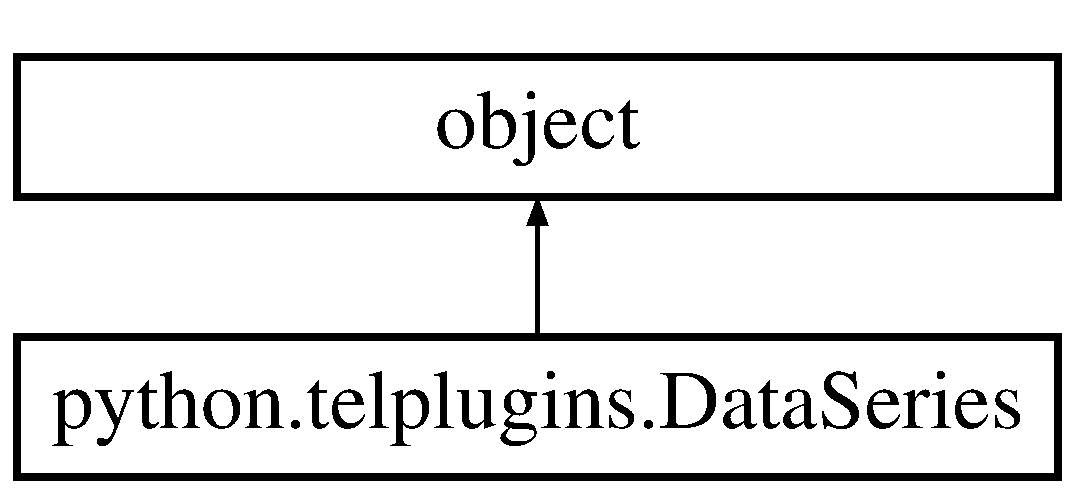
\includegraphics[height=2.000000cm]{classpython_1_1telplugins_1_1_data_series}
\end{center}
\end{figure}
\subsection*{Public Member Functions}
\begin{DoxyCompactItemize}
\item 
def \hyperlink{classpython_1_1telplugins_1_1_data_series_aa29eec3b2aa8cd3b2b0a4c4316325e10}{\-\_\-\-\_\-init\-\_\-\-\_\-}
\begin{DoxyCompactList}\small\item\em Constructor for \hyperlink{classpython_1_1telplugins_1_1_data_series}{Data\-Series} class. \end{DoxyCompactList}\item 
\hypertarget{classpython_1_1telplugins_1_1_data_series_abc33f2a0ecd52e6f28f47fe86a9e37b5}{def {\bfseries from\-Num\-Py}}\label{classpython_1_1telplugins_1_1_data_series_abc33f2a0ecd52e6f28f47fe86a9e37b5}

\item 
\hypertarget{classpython_1_1telplugins_1_1_data_series_ad4944df5b1f228d59f1e0b89d89424e3}{def {\bfseries \-\_\-\-\_\-del\-\_\-\-\_\-}}\label{classpython_1_1telplugins_1_1_data_series_ad4944df5b1f228d59f1e0b89d89424e3}

\item 
def \hyperlink{classpython_1_1telplugins_1_1_data_series_ace23540a192e59586d4fcf14bb96833f}{get\-Column\-Headers}
\begin{DoxyCompactList}\small\item\em Retrive the column headers as a list. \end{DoxyCompactList}\item 
def \hyperlink{classpython_1_1telplugins_1_1_data_series_a0c2c08ce2d865d58bb8e9661ba55658d}{get\-Element}
\begin{DoxyCompactList}\small\item\em Get a specific element from a dataseries. \end{DoxyCompactList}\item 
def \hyperlink{classpython_1_1telplugins_1_1_data_series_a9886e132dcfc46c715201247b0c1bc7e}{set\-Element}
\begin{DoxyCompactList}\small\item\em Set a specific element. \end{DoxyCompactList}\item 
def \hyperlink{classpython_1_1telplugins_1_1_data_series_a65b2933d24a5ffb2aa123baae6364cf2}{read\-Data\-Series}
\begin{DoxyCompactList}\small\item\em Read a dataseries from a file. \end{DoxyCompactList}\item 
def \hyperlink{classpython_1_1telplugins_1_1_data_series_a79c406248945414b6b7d78556d6cb00d}{write\-Data\-Series}
\begin{DoxyCompactList}\small\item\em Write a dataseries to a file. \end{DoxyCompactList}\item 
def \hyperlink{classpython_1_1telplugins_1_1_data_series_aeb8e4daabd433513f8261dcd2e788c74}{plot}
\begin{DoxyCompactList}\small\item\em Plot a dataseries as a graph. \end{DoxyCompactList}\end{DoxyCompactItemize}
\subsection*{Properties}
\begin{DoxyCompactItemize}
\item 
\hypertarget{classpython_1_1telplugins_1_1_data_series_a484661d2e01e165fa84cfdf528d76276}{{\bfseries data} = property(\-\_\-\-\_\-get\-Handle)}\label{classpython_1_1telplugins_1_1_data_series_a484661d2e01e165fa84cfdf528d76276}

\item 
\hyperlink{classpython_1_1telplugins_1_1_data_series_a82084dee126303cc0322e31e48239e76}{to\-Numpy} = property(\-\_\-\-\_\-to\-Numpy)
\begin{DoxyCompactList}\small\item\em Return a numpy array from a data series. \end{DoxyCompactList}\item 
\hyperlink{classpython_1_1telplugins_1_1_data_series_a79a79ef89d47682c0fcc0620d1bf21b5}{rows} = property(\-\_\-\-\_\-get\-Number\-Of\-Rows)
\begin{DoxyCompactList}\small\item\em Return the number of rows in the data series. \end{DoxyCompactList}\item 
\hyperlink{classpython_1_1telplugins_1_1_data_series_afb458f814018a15446b32052d4d2b4cf}{cols} = property(\-\_\-\-\_\-get\-Number\-Of\-Columns)
\begin{DoxyCompactList}\small\item\em Return the number of columns in the data series. \end{DoxyCompactList}\end{DoxyCompactItemize}


\subsection{Detailed Description}
\hyperlink{classpython_1_1telplugins_1_1_data_series}{Data\-Series} class for handling roadrunner data types. 

\subsection{Constructor \& Destructor Documentation}
\hypertarget{classpython_1_1telplugins_1_1_data_series_aa29eec3b2aa8cd3b2b0a4c4316325e10}{\index{python\-::telplugins\-::\-Data\-Series@{python\-::telplugins\-::\-Data\-Series}!\-\_\-\-\_\-init\-\_\-\-\_\-@{\-\_\-\-\_\-init\-\_\-\-\_\-}}
\index{\-\_\-\-\_\-init\-\_\-\-\_\-@{\-\_\-\-\_\-init\-\_\-\-\_\-}!python::telplugins::DataSeries@{python\-::telplugins\-::\-Data\-Series}}
\subsubsection[{\-\_\-\-\_\-init\-\_\-\-\_\-}]{\setlength{\rightskip}{0pt plus 5cm}def python.\-telplugins.\-Data\-Series.\-\_\-\-\_\-init\-\_\-\-\_\- (
\begin{DoxyParamCaption}
\item[{}]{self, }
\item[{}]{handle = {\ttfamily None}, }
\item[{}]{my\-Data = {\ttfamily False}}
\end{DoxyParamCaption}
)}}\label{classpython_1_1telplugins_1_1_data_series_aa29eec3b2aa8cd3b2b0a4c4316325e10}


Constructor for \hyperlink{classpython_1_1telplugins_1_1_data_series}{Data\-Series} class. 


\begin{DoxyCode}
1 d = DataSeries()
2 d = DataSeries (rr)
\end{DoxyCode}
 

\subsection{Member Function Documentation}
\hypertarget{classpython_1_1telplugins_1_1_data_series_ace23540a192e59586d4fcf14bb96833f}{\index{python\-::telplugins\-::\-Data\-Series@{python\-::telplugins\-::\-Data\-Series}!get\-Column\-Headers@{get\-Column\-Headers}}
\index{get\-Column\-Headers@{get\-Column\-Headers}!python::telplugins::DataSeries@{python\-::telplugins\-::\-Data\-Series}}
\subsubsection[{get\-Column\-Headers}]{\setlength{\rightskip}{0pt plus 5cm}def python.\-telplugins.\-Data\-Series.\-get\-Column\-Headers (
\begin{DoxyParamCaption}
\item[{}]{self}
\end{DoxyParamCaption}
)}}\label{classpython_1_1telplugins_1_1_data_series_ace23540a192e59586d4fcf14bb96833f}


Retrive the column headers as a list. 


\begin{DoxyCode}
1 \textcolor{keywordflow}{print} d.getColumnHeaders()
\end{DoxyCode}
 \hypertarget{classpython_1_1telplugins_1_1_data_series_a0c2c08ce2d865d58bb8e9661ba55658d}{\index{python\-::telplugins\-::\-Data\-Series@{python\-::telplugins\-::\-Data\-Series}!get\-Element@{get\-Element}}
\index{get\-Element@{get\-Element}!python::telplugins::DataSeries@{python\-::telplugins\-::\-Data\-Series}}
\subsubsection[{get\-Element}]{\setlength{\rightskip}{0pt plus 5cm}def python.\-telplugins.\-Data\-Series.\-get\-Element (
\begin{DoxyParamCaption}
\item[{}]{self, }
\item[{}]{row, }
\item[{}]{col}
\end{DoxyParamCaption}
)}}\label{classpython_1_1telplugins_1_1_data_series_a0c2c08ce2d865d58bb8e9661ba55658d}


Get a specific element from a dataseries. 


\begin{DoxyCode}
1 \textcolor{keywordflow}{print} d.getElement (1,2)
\end{DoxyCode}
 \hypertarget{classpython_1_1telplugins_1_1_data_series_aeb8e4daabd433513f8261dcd2e788c74}{\index{python\-::telplugins\-::\-Data\-Series@{python\-::telplugins\-::\-Data\-Series}!plot@{plot}}
\index{plot@{plot}!python::telplugins::DataSeries@{python\-::telplugins\-::\-Data\-Series}}
\subsubsection[{plot}]{\setlength{\rightskip}{0pt plus 5cm}def python.\-telplugins.\-Data\-Series.\-plot (
\begin{DoxyParamCaption}
\item[{}]{self}
\end{DoxyParamCaption}
)}}\label{classpython_1_1telplugins_1_1_data_series_aeb8e4daabd433513f8261dcd2e788c74}


Plot a dataseries as a graph. 


\begin{DoxyCode}
1 d.plot()
\end{DoxyCode}
 \hypertarget{classpython_1_1telplugins_1_1_data_series_a65b2933d24a5ffb2aa123baae6364cf2}{\index{python\-::telplugins\-::\-Data\-Series@{python\-::telplugins\-::\-Data\-Series}!read\-Data\-Series@{read\-Data\-Series}}
\index{read\-Data\-Series@{read\-Data\-Series}!python::telplugins::DataSeries@{python\-::telplugins\-::\-Data\-Series}}
\subsubsection[{read\-Data\-Series}]{\setlength{\rightskip}{0pt plus 5cm}def python.\-telplugins.\-Data\-Series.\-read\-Data\-Series (
\begin{DoxyParamCaption}
\item[{}]{cls, }
\item[{}]{file\-Name}
\end{DoxyParamCaption}
)}}\label{classpython_1_1telplugins_1_1_data_series_a65b2933d24a5ffb2aa123baae6364cf2}


Read a dataseries from a file. 


\begin{DoxyCode}
1 d.readDataSeries (\textcolor{stringliteral}{"myDataSeries.txt"})
\end{DoxyCode}
 \hypertarget{classpython_1_1telplugins_1_1_data_series_a9886e132dcfc46c715201247b0c1bc7e}{\index{python\-::telplugins\-::\-Data\-Series@{python\-::telplugins\-::\-Data\-Series}!set\-Element@{set\-Element}}
\index{set\-Element@{set\-Element}!python::telplugins::DataSeries@{python\-::telplugins\-::\-Data\-Series}}
\subsubsection[{set\-Element}]{\setlength{\rightskip}{0pt plus 5cm}def python.\-telplugins.\-Data\-Series.\-set\-Element (
\begin{DoxyParamCaption}
\item[{}]{self, }
\item[{}]{row, }
\item[{}]{col, }
\item[{}]{value}
\end{DoxyParamCaption}
)}}\label{classpython_1_1telplugins_1_1_data_series_a9886e132dcfc46c715201247b0c1bc7e}


Set a specific element. 


\begin{DoxyCode}
1 d.setElement (1,2, 3.1415)
\end{DoxyCode}
 \hypertarget{classpython_1_1telplugins_1_1_data_series_a79c406248945414b6b7d78556d6cb00d}{\index{python\-::telplugins\-::\-Data\-Series@{python\-::telplugins\-::\-Data\-Series}!write\-Data\-Series@{write\-Data\-Series}}
\index{write\-Data\-Series@{write\-Data\-Series}!python::telplugins::DataSeries@{python\-::telplugins\-::\-Data\-Series}}
\subsubsection[{write\-Data\-Series}]{\setlength{\rightskip}{0pt plus 5cm}def python.\-telplugins.\-Data\-Series.\-write\-Data\-Series (
\begin{DoxyParamCaption}
\item[{}]{self, }
\item[{}]{file\-Name}
\end{DoxyParamCaption}
)}}\label{classpython_1_1telplugins_1_1_data_series_a79c406248945414b6b7d78556d6cb00d}


Write a dataseries to a file. 


\begin{DoxyCode}
1 d.writeDataSeries (\textcolor{stringliteral}{"myDataSeries.txt"})
\end{DoxyCode}
 

\subsection{Property Documentation}
\hypertarget{classpython_1_1telplugins_1_1_data_series_afb458f814018a15446b32052d4d2b4cf}{\index{python\-::telplugins\-::\-Data\-Series@{python\-::telplugins\-::\-Data\-Series}!cols@{cols}}
\index{cols@{cols}!python::telplugins::DataSeries@{python\-::telplugins\-::\-Data\-Series}}
\subsubsection[{cols}]{\setlength{\rightskip}{0pt plus 5cm}python.\-telplugins.\-Data\-Series.\-cols = property(\-\_\-\-\_\-get\-Number\-Of\-Columns)\hspace{0.3cm}{\ttfamily [static]}}}\label{classpython_1_1telplugins_1_1_data_series_afb458f814018a15446b32052d4d2b4cf}


Return the number of columns in the data series. 


\begin{DoxyCode}
1 \textcolor{keywordflow}{print} d.cols
\end{DoxyCode}
 \hypertarget{classpython_1_1telplugins_1_1_data_series_a79a79ef89d47682c0fcc0620d1bf21b5}{\index{python\-::telplugins\-::\-Data\-Series@{python\-::telplugins\-::\-Data\-Series}!rows@{rows}}
\index{rows@{rows}!python::telplugins::DataSeries@{python\-::telplugins\-::\-Data\-Series}}
\subsubsection[{rows}]{\setlength{\rightskip}{0pt plus 5cm}python.\-telplugins.\-Data\-Series.\-rows = property(\-\_\-\-\_\-get\-Number\-Of\-Rows)\hspace{0.3cm}{\ttfamily [static]}}}\label{classpython_1_1telplugins_1_1_data_series_a79a79ef89d47682c0fcc0620d1bf21b5}


Return the number of rows in the data series. 


\begin{DoxyCode}
1 \textcolor{keywordflow}{print} d.rows
\end{DoxyCode}
 \hypertarget{classpython_1_1telplugins_1_1_data_series_a82084dee126303cc0322e31e48239e76}{\index{python\-::telplugins\-::\-Data\-Series@{python\-::telplugins\-::\-Data\-Series}!to\-Numpy@{to\-Numpy}}
\index{to\-Numpy@{to\-Numpy}!python::telplugins::DataSeries@{python\-::telplugins\-::\-Data\-Series}}
\subsubsection[{to\-Numpy}]{\setlength{\rightskip}{0pt plus 5cm}python.\-telplugins.\-Data\-Series.\-to\-Numpy = property(\-\_\-\-\_\-to\-Numpy)\hspace{0.3cm}{\ttfamily [static]}}}\label{classpython_1_1telplugins_1_1_data_series_a82084dee126303cc0322e31e48239e76}


Return a numpy array from a data series. 


\begin{DoxyCode}
1 myarray = d.toNumpy
\end{DoxyCode}
 

The documentation for this class was generated from the following file\-:\begin{DoxyCompactItemize}
\item 
telplugins.\-py\end{DoxyCompactItemize}

\hypertarget{classpython_1_1telplugins_1_1_event}{\section{python.\-telplugins.\-Event Class Reference}
\label{classpython_1_1telplugins_1_1_event}\index{python.\-telplugins.\-Event@{python.\-telplugins.\-Event}}
}
Inheritance diagram for python.\-telplugins.\-Event\-:\begin{figure}[H]
\begin{center}
\leavevmode
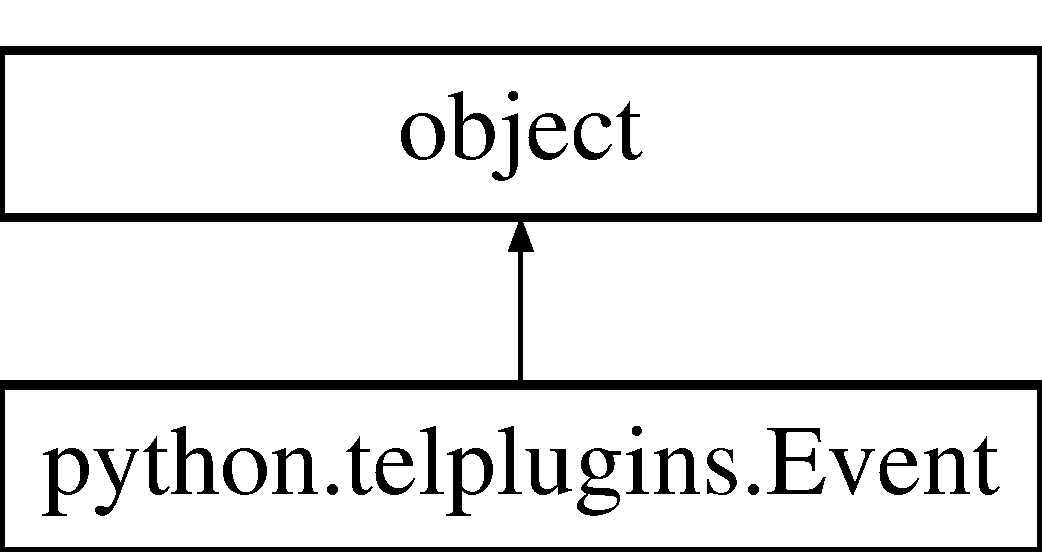
\includegraphics[height=2.000000cm]{classpython_1_1telplugins_1_1_event}
\end{center}
\end{figure}
\subsection*{Public Member Functions}
\begin{DoxyCompactItemize}
\item 
\hypertarget{classpython_1_1telplugins_1_1_event_a484bfa984ab105ff6ad449d20d09314a}{def {\bfseries \-\_\-\-\_\-init\-\_\-\-\_\-}}\label{classpython_1_1telplugins_1_1_event_a484bfa984ab105ff6ad449d20d09314a}

\item 
\hypertarget{classpython_1_1telplugins_1_1_event_ae4ccc23552c51df57dc1b77bfabcbb7e}{def {\bfseries add}}\label{classpython_1_1telplugins_1_1_event_ae4ccc23552c51df57dc1b77bfabcbb7e}

\item 
\hypertarget{classpython_1_1telplugins_1_1_event_afe249d309b85952f8f87ebf78e2227b1}{def {\bfseries remove}}\label{classpython_1_1telplugins_1_1_event_afe249d309b85952f8f87ebf78e2227b1}

\item 
\hypertarget{classpython_1_1telplugins_1_1_event_a038ac78d0d08e23c39671071e56ace72}{def {\bfseries fire}}\label{classpython_1_1telplugins_1_1_event_a038ac78d0d08e23c39671071e56ace72}

\end{DoxyCompactItemize}
\subsection*{Public Attributes}
\begin{DoxyCompactItemize}
\item 
\hypertarget{classpython_1_1telplugins_1_1_event_a5d2a24fa4fa288afb4416ab85a4f3fc3}{{\bfseries handlers}}\label{classpython_1_1telplugins_1_1_event_a5d2a24fa4fa288afb4416ab85a4f3fc3}

\end{DoxyCompactItemize}


The documentation for this class was generated from the following file\-:\begin{DoxyCompactItemize}
\item 
telplugins.\-py\end{DoxyCompactItemize}

\hypertarget{classpython_1_1telplugins_1_1_plugin}{\section{python.\-telplugins.\-Plugin Class Reference}
\label{classpython_1_1telplugins_1_1_plugin}\index{python.\-telplugins.\-Plugin@{python.\-telplugins.\-Plugin}}
}
Inheritance diagram for python.\-telplugins.\-Plugin\-:\begin{figure}[H]
\begin{center}
\leavevmode
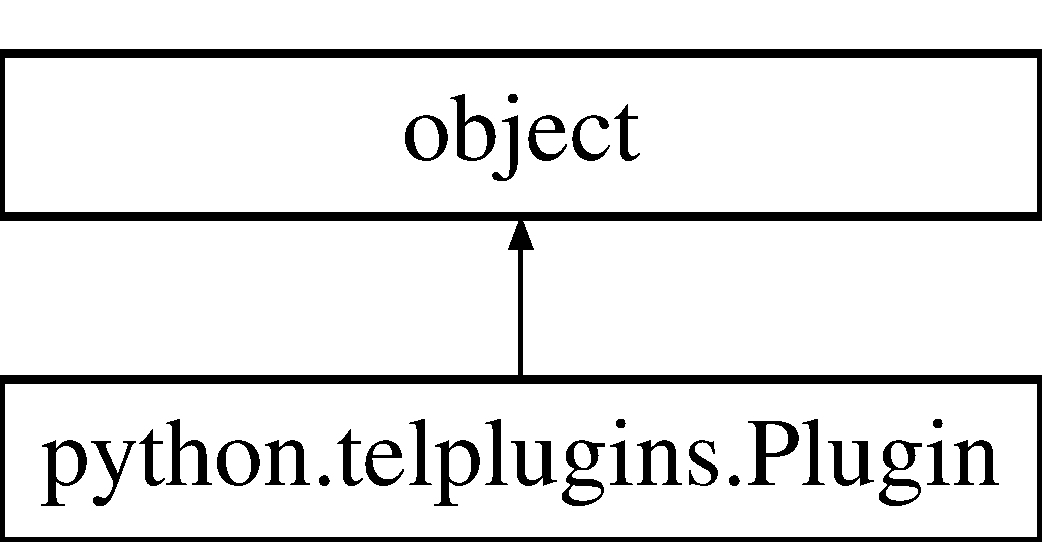
\includegraphics[height=2.000000cm]{classpython_1_1telplugins_1_1_plugin}
\end{center}
\end{figure}
\subsection*{Public Member Functions}
\begin{DoxyCompactItemize}
\item 
def \hyperlink{classpython_1_1telplugins_1_1_plugin_ac7c01bc2430411e784d753af124ebf91}{\-\_\-\-\_\-init\-\_\-\-\_\-}
\begin{DoxyCompactList}\small\item\em Create a \hyperlink{classpython_1_1telplugins_1_1_plugin}{Plugin} instance. \end{DoxyCompactList}\item 
def \hyperlink{classpython_1_1telplugins_1_1_plugin_aaa65888e8585ed3465efb885ef1a724d}{set\-Property}
\begin{DoxyCompactList}\small\item\em Set a given propoerty in the plugin. \end{DoxyCompactList}\item 
def \hyperlink{classpython_1_1telplugins_1_1_plugin_aaeaf0cdf9fd98f2386add1282e18bde3}{get\-Property}
\begin{DoxyCompactList}\small\item\em Get the value for a given propoerty in the plugin. \end{DoxyCompactList}\item 
\hypertarget{classpython_1_1telplugins_1_1_plugin_a029387a4e029c2d5740b42251696601d}{def {\bfseries \-\_\-\-\_\-setattr\-\_\-\-\_\-}}\label{classpython_1_1telplugins_1_1_plugin_a029387a4e029c2d5740b42251696601d}

\item 
\hypertarget{classpython_1_1telplugins_1_1_plugin_a39c2932fb05d2c661cf1ae7e1f5c9c18}{def {\bfseries \-\_\-\-\_\-getattr\-\_\-\-\_\-}}\label{classpython_1_1telplugins_1_1_plugin_a39c2932fb05d2c661cf1ae7e1f5c9c18}

\item 
def \hyperlink{classpython_1_1telplugins_1_1_plugin_a164f3353a5011ce929692e8c245f36c5}{list\-Of\-Properties}
\begin{DoxyCompactList}\small\item\em List all the properties in the plugin. \end{DoxyCompactList}\item 
def \hyperlink{classpython_1_1telplugins_1_1_plugin_a5ff6c70a0d04ae143d793aed7e47fed9}{list\-Of\-Property\-Descriptions}
\begin{DoxyCompactList}\small\item\em List all the property descriptions in the plugin. \end{DoxyCompactList}\item 
def \hyperlink{classpython_1_1telplugins_1_1_plugin_a7b07b2142cbc9384823f99cbef9c0edf}{list\-Of\-Property\-Hints}
\begin{DoxyCompactList}\small\item\em List all the property hints in the plugin. \end{DoxyCompactList}\item 
def \hyperlink{classpython_1_1telplugins_1_1_plugin_a185e216badc55e248976d4811f3c0844}{load\-Data\-Series\-As\-Num\-Py}
\begin{DoxyCompactList}\small\item\em List all the property hints in the plugin. \end{DoxyCompactList}\item 
\hypertarget{classpython_1_1telplugins_1_1_plugin_a5cf2b8d5c72067970b0b9e642fbb62b3}{def {\bfseries On\-Progress}}\label{classpython_1_1telplugins_1_1_plugin_a5cf2b8d5c72067970b0b9e642fbb62b3}

\item 
def \hyperlink{classpython_1_1telplugins_1_1_plugin_a0507c60e5a2ee11ac648433f79fe3e97}{execute}
\begin{DoxyCompactList}\small\item\em Execute the plugin. \end{DoxyCompactList}\item 
\hypertarget{classpython_1_1telplugins_1_1_plugin_ab3d71fa2c9787e1ad70be02aa015c64e}{def {\bfseries execute\-Ex}}\label{classpython_1_1telplugins_1_1_plugin_ab3d71fa2c9787e1ad70be02aa015c64e}

\item 
def \hyperlink{classpython_1_1telplugins_1_1_plugin_a6166ea0c8583ef1b560d1d46f7fb9ac6}{read\-All\-Text}
\begin{DoxyCompactList}\small\item\em Read all text from a file. \end{DoxyCompactList}\item 
\hypertarget{classpython_1_1telplugins_1_1_plugin_a629762005804234265ff6687e3a64982}{def {\bfseries load\-Plugins}}\label{classpython_1_1telplugins_1_1_plugin_a629762005804234265ff6687e3a64982}

\item 
def \hyperlink{classpython_1_1telplugins_1_1_plugin_a99dc50fd956142906ac7106651e6ace7}{view\-Manual}
\begin{DoxyCompactList}\small\item\em If a plugin has a manual, view it. \end{DoxyCompactList}\item 
def \hyperlink{classpython_1_1telplugins_1_1_plugin_a0cb4a44fda678bd2057ab99208a355bb}{name}
\begin{DoxyCompactList}\small\item\em Returns the name of the plugin. \end{DoxyCompactList}\item 
def \hyperlink{classpython_1_1telplugins_1_1_plugin_a2358ed8d643666b29b97047dd762dccb}{description}
\begin{DoxyCompactList}\small\item\em Returns the description of the plugin. \end{DoxyCompactList}\item 
def \hyperlink{classpython_1_1telplugins_1_1_plugin_a642879901179a21744afed441590f813}{hint}
\begin{DoxyCompactList}\small\item\em Returns the hint of the plugin. \end{DoxyCompactList}\item 
\hypertarget{classpython_1_1telplugins_1_1_plugin_af711f0571a86bf4dcd598b5ed8455a98}{def {\bfseries info}}\label{classpython_1_1telplugins_1_1_plugin_af711f0571a86bf4dcd598b5ed8455a98}

\end{DoxyCompactItemize}
\subsection*{Static Public Member Functions}
\begin{DoxyCompactItemize}
\item 
def \hyperlink{classpython_1_1telplugins_1_1_plugin_a3a980445c8df1cb8441167ded08af590}{list\-Of\-Plugins}
\begin{DoxyCompactList}\small\item\em Static method to list all plugins. \end{DoxyCompactList}\end{DoxyCompactItemize}
\subsection*{Public Attributes}
\begin{DoxyCompactItemize}
\item 
\hypertarget{classpython_1_1telplugins_1_1_plugin_a27ec760a754e8f5fd3e9d59eae657a53}{{\bfseries plugin\-Name}}\label{classpython_1_1telplugins_1_1_plugin_a27ec760a754e8f5fd3e9d59eae657a53}

\item 
\hypertarget{classpython_1_1telplugins_1_1_plugin_a03e678a5dd28fff76d2e8909c29eced4}{{\bfseries plugin}}\label{classpython_1_1telplugins_1_1_plugin_a03e678a5dd28fff76d2e8909c29eced4}

\end{DoxyCompactItemize}


\subsection{Constructor \& Destructor Documentation}
\hypertarget{classpython_1_1telplugins_1_1_plugin_ac7c01bc2430411e784d753af124ebf91}{\index{python\-::telplugins\-::\-Plugin@{python\-::telplugins\-::\-Plugin}!\-\_\-\-\_\-init\-\_\-\-\_\-@{\-\_\-\-\_\-init\-\_\-\-\_\-}}
\index{\-\_\-\-\_\-init\-\_\-\-\_\-@{\-\_\-\-\_\-init\-\_\-\-\_\-}!python::telplugins::Plugin@{python\-::telplugins\-::\-Plugin}}
\subsubsection[{\-\_\-\-\_\-init\-\_\-\-\_\-}]{\setlength{\rightskip}{0pt plus 5cm}def python.\-telplugins.\-Plugin.\-\_\-\-\_\-init\-\_\-\-\_\- (
\begin{DoxyParamCaption}
\item[{}]{self, }
\item[{}]{plugin\-Name}
\end{DoxyParamCaption}
)}}\label{classpython_1_1telplugins_1_1_plugin_ac7c01bc2430411e784d753af124ebf91}


Create a \hyperlink{classpython_1_1telplugins_1_1_plugin}{Plugin} instance. 


\begin{DoxyCode}
1 myPlugin = Plugin (\textcolor{stringliteral}{"tel\_add\_noise"})
\end{DoxyCode}
 

\subsection{Member Function Documentation}
\hypertarget{classpython_1_1telplugins_1_1_plugin_a2358ed8d643666b29b97047dd762dccb}{\index{python\-::telplugins\-::\-Plugin@{python\-::telplugins\-::\-Plugin}!description@{description}}
\index{description@{description}!python::telplugins::Plugin@{python\-::telplugins\-::\-Plugin}}
\subsubsection[{description}]{\setlength{\rightskip}{0pt plus 5cm}def python.\-telplugins.\-Plugin.\-description (
\begin{DoxyParamCaption}
\item[{}]{self}
\end{DoxyParamCaption}
)}}\label{classpython_1_1telplugins_1_1_plugin_a2358ed8d643666b29b97047dd762dccb}


Returns the description of the plugin. 


\begin{DoxyCode}
1 \textcolor{keywordflow}{print} myPlugin.description()
\end{DoxyCode}
 \hypertarget{classpython_1_1telplugins_1_1_plugin_a0507c60e5a2ee11ac648433f79fe3e97}{\index{python\-::telplugins\-::\-Plugin@{python\-::telplugins\-::\-Plugin}!execute@{execute}}
\index{execute@{execute}!python::telplugins::Plugin@{python\-::telplugins\-::\-Plugin}}
\subsubsection[{execute}]{\setlength{\rightskip}{0pt plus 5cm}def python.\-telplugins.\-Plugin.\-execute (
\begin{DoxyParamCaption}
\item[{}]{self}
\end{DoxyParamCaption}
)}}\label{classpython_1_1telplugins_1_1_plugin_a0507c60e5a2ee11ac648433f79fe3e97}


Execute the plugin. 


\begin{DoxyCode}
1 \textcolor{keywordflow}{print} myPlugin.execute()
\end{DoxyCode}
 \hypertarget{classpython_1_1telplugins_1_1_plugin_aaeaf0cdf9fd98f2386add1282e18bde3}{\index{python\-::telplugins\-::\-Plugin@{python\-::telplugins\-::\-Plugin}!get\-Property@{get\-Property}}
\index{get\-Property@{get\-Property}!python::telplugins::Plugin@{python\-::telplugins\-::\-Plugin}}
\subsubsection[{get\-Property}]{\setlength{\rightskip}{0pt plus 5cm}def python.\-telplugins.\-Plugin.\-get\-Property (
\begin{DoxyParamCaption}
\item[{}]{self, }
\item[{}]{name}
\end{DoxyParamCaption}
)}}\label{classpython_1_1telplugins_1_1_plugin_aaeaf0cdf9fd98f2386add1282e18bde3}


Get the value for a given propoerty in the plugin. 


\begin{DoxyCode}
1 \textcolor{keywordflow}{print} myPlugin.getProperty(\textcolor{stringliteral}{"Sigma"})
\end{DoxyCode}
 \hypertarget{classpython_1_1telplugins_1_1_plugin_a642879901179a21744afed441590f813}{\index{python\-::telplugins\-::\-Plugin@{python\-::telplugins\-::\-Plugin}!hint@{hint}}
\index{hint@{hint}!python::telplugins::Plugin@{python\-::telplugins\-::\-Plugin}}
\subsubsection[{hint}]{\setlength{\rightskip}{0pt plus 5cm}def python.\-telplugins.\-Plugin.\-hint (
\begin{DoxyParamCaption}
\item[{}]{self}
\end{DoxyParamCaption}
)}}\label{classpython_1_1telplugins_1_1_plugin_a642879901179a21744afed441590f813}


Returns the hint of the plugin. 


\begin{DoxyCode}
1 \textcolor{keywordflow}{print} myPlugin.hint()
\end{DoxyCode}
 \hypertarget{classpython_1_1telplugins_1_1_plugin_a3a980445c8df1cb8441167ded08af590}{\index{python\-::telplugins\-::\-Plugin@{python\-::telplugins\-::\-Plugin}!list\-Of\-Plugins@{list\-Of\-Plugins}}
\index{list\-Of\-Plugins@{list\-Of\-Plugins}!python::telplugins::Plugin@{python\-::telplugins\-::\-Plugin}}
\subsubsection[{list\-Of\-Plugins}]{\setlength{\rightskip}{0pt plus 5cm}def python.\-telplugins.\-Plugin.\-list\-Of\-Plugins (
\begin{DoxyParamCaption}
{}
\end{DoxyParamCaption}
)\hspace{0.3cm}{\ttfamily [static]}}}\label{classpython_1_1telplugins_1_1_plugin_a3a980445c8df1cb8441167ded08af590}


Static method to list all plugins. 


\begin{DoxyCode}
1 \textcolor{keywordflow}{print} Plugin.listOfPlugins()
\end{DoxyCode}
 \hypertarget{classpython_1_1telplugins_1_1_plugin_a164f3353a5011ce929692e8c245f36c5}{\index{python\-::telplugins\-::\-Plugin@{python\-::telplugins\-::\-Plugin}!list\-Of\-Properties@{list\-Of\-Properties}}
\index{list\-Of\-Properties@{list\-Of\-Properties}!python::telplugins::Plugin@{python\-::telplugins\-::\-Plugin}}
\subsubsection[{list\-Of\-Properties}]{\setlength{\rightskip}{0pt plus 5cm}def python.\-telplugins.\-Plugin.\-list\-Of\-Properties (
\begin{DoxyParamCaption}
\item[{}]{self}
\end{DoxyParamCaption}
)}}\label{classpython_1_1telplugins_1_1_plugin_a164f3353a5011ce929692e8c245f36c5}


List all the properties in the plugin. 


\begin{DoxyCode}
1 \textcolor{keywordflow}{print} myPlugin.listOfProperties()
\end{DoxyCode}
 \hypertarget{classpython_1_1telplugins_1_1_plugin_a5ff6c70a0d04ae143d793aed7e47fed9}{\index{python\-::telplugins\-::\-Plugin@{python\-::telplugins\-::\-Plugin}!list\-Of\-Property\-Descriptions@{list\-Of\-Property\-Descriptions}}
\index{list\-Of\-Property\-Descriptions@{list\-Of\-Property\-Descriptions}!python::telplugins::Plugin@{python\-::telplugins\-::\-Plugin}}
\subsubsection[{list\-Of\-Property\-Descriptions}]{\setlength{\rightskip}{0pt plus 5cm}def python.\-telplugins.\-Plugin.\-list\-Of\-Property\-Descriptions (
\begin{DoxyParamCaption}
\item[{}]{self}
\end{DoxyParamCaption}
)}}\label{classpython_1_1telplugins_1_1_plugin_a5ff6c70a0d04ae143d793aed7e47fed9}


List all the property descriptions in the plugin. 


\begin{DoxyCode}
1 \textcolor{keywordflow}{print} myPlugin.listOfPropertyDescriptions()
\end{DoxyCode}
 
\begin{DoxyCode}
1 \textcolor{keyword}{import} pprint
2 \textcolor{keywordflow}{print} pprint.pprint (na.listOfProperties())  
\end{DoxyCode}
 \hypertarget{classpython_1_1telplugins_1_1_plugin_a7b07b2142cbc9384823f99cbef9c0edf}{\index{python\-::telplugins\-::\-Plugin@{python\-::telplugins\-::\-Plugin}!list\-Of\-Property\-Hints@{list\-Of\-Property\-Hints}}
\index{list\-Of\-Property\-Hints@{list\-Of\-Property\-Hints}!python::telplugins::Plugin@{python\-::telplugins\-::\-Plugin}}
\subsubsection[{list\-Of\-Property\-Hints}]{\setlength{\rightskip}{0pt plus 5cm}def python.\-telplugins.\-Plugin.\-list\-Of\-Property\-Hints (
\begin{DoxyParamCaption}
\item[{}]{self}
\end{DoxyParamCaption}
)}}\label{classpython_1_1telplugins_1_1_plugin_a7b07b2142cbc9384823f99cbef9c0edf}


List all the property hints in the plugin. 


\begin{DoxyCode}
1 \textcolor{keywordflow}{print} myPlugin.listOfPropertyHints()
\end{DoxyCode}
 \hypertarget{classpython_1_1telplugins_1_1_plugin_a185e216badc55e248976d4811f3c0844}{\index{python\-::telplugins\-::\-Plugin@{python\-::telplugins\-::\-Plugin}!load\-Data\-Series\-As\-Num\-Py@{load\-Data\-Series\-As\-Num\-Py}}
\index{load\-Data\-Series\-As\-Num\-Py@{load\-Data\-Series\-As\-Num\-Py}!python::telplugins::Plugin@{python\-::telplugins\-::\-Plugin}}
\subsubsection[{load\-Data\-Series\-As\-Num\-Py}]{\setlength{\rightskip}{0pt plus 5cm}def python.\-telplugins.\-Plugin.\-load\-Data\-Series\-As\-Num\-Py (
\begin{DoxyParamCaption}
\item[{}]{self, }
\item[{}]{file\-Name}
\end{DoxyParamCaption}
)}}\label{classpython_1_1telplugins_1_1_plugin_a185e216badc55e248976d4811f3c0844}


List all the property hints in the plugin. 


\begin{DoxyCode}
1 \textcolor{keywordflow}{print} myPlugin.listOfPropertyHints()
\end{DoxyCode}
 \hypertarget{classpython_1_1telplugins_1_1_plugin_a0cb4a44fda678bd2057ab99208a355bb}{\index{python\-::telplugins\-::\-Plugin@{python\-::telplugins\-::\-Plugin}!name@{name}}
\index{name@{name}!python::telplugins::Plugin@{python\-::telplugins\-::\-Plugin}}
\subsubsection[{name}]{\setlength{\rightskip}{0pt plus 5cm}def python.\-telplugins.\-Plugin.\-name (
\begin{DoxyParamCaption}
\item[{}]{self}
\end{DoxyParamCaption}
)}}\label{classpython_1_1telplugins_1_1_plugin_a0cb4a44fda678bd2057ab99208a355bb}


Returns the name of the plugin. 


\begin{DoxyCode}
1 \textcolor{keywordflow}{print} myPlugin.name()
\end{DoxyCode}
 \hypertarget{classpython_1_1telplugins_1_1_plugin_a6166ea0c8583ef1b560d1d46f7fb9ac6}{\index{python\-::telplugins\-::\-Plugin@{python\-::telplugins\-::\-Plugin}!read\-All\-Text@{read\-All\-Text}}
\index{read\-All\-Text@{read\-All\-Text}!python::telplugins::Plugin@{python\-::telplugins\-::\-Plugin}}
\subsubsection[{read\-All\-Text}]{\setlength{\rightskip}{0pt plus 5cm}def python.\-telplugins.\-Plugin.\-read\-All\-Text (
\begin{DoxyParamCaption}
\item[{}]{self, }
\item[{}]{f\-Name}
\end{DoxyParamCaption}
)}}\label{classpython_1_1telplugins_1_1_plugin_a6166ea0c8583ef1b560d1d46f7fb9ac6}


Read all text from a file. 


\begin{DoxyCode}
1 \textcolor{keywordflow}{print} myplugin.readAllText (\textcolor{stringliteral}{"myfile.txt"})
\end{DoxyCode}
 \hypertarget{classpython_1_1telplugins_1_1_plugin_aaa65888e8585ed3465efb885ef1a724d}{\index{python\-::telplugins\-::\-Plugin@{python\-::telplugins\-::\-Plugin}!set\-Property@{set\-Property}}
\index{set\-Property@{set\-Property}!python::telplugins::Plugin@{python\-::telplugins\-::\-Plugin}}
\subsubsection[{set\-Property}]{\setlength{\rightskip}{0pt plus 5cm}def python.\-telplugins.\-Plugin.\-set\-Property (
\begin{DoxyParamCaption}
\item[{}]{self, }
\item[{}]{name, }
\item[{}]{value}
\end{DoxyParamCaption}
)}}\label{classpython_1_1telplugins_1_1_plugin_aaa65888e8585ed3465efb885ef1a724d}


Set a given propoerty in the plugin. 


\begin{DoxyCode}
1 myPlugin.setProperty (\textcolor{stringliteral}{"Sigma"}, 0.1)
\end{DoxyCode}
 \hypertarget{classpython_1_1telplugins_1_1_plugin_a99dc50fd956142906ac7106651e6ace7}{\index{python\-::telplugins\-::\-Plugin@{python\-::telplugins\-::\-Plugin}!view\-Manual@{view\-Manual}}
\index{view\-Manual@{view\-Manual}!python::telplugins::Plugin@{python\-::telplugins\-::\-Plugin}}
\subsubsection[{view\-Manual}]{\setlength{\rightskip}{0pt plus 5cm}def python.\-telplugins.\-Plugin.\-view\-Manual (
\begin{DoxyParamCaption}
\item[{}]{self}
\end{DoxyParamCaption}
)}}\label{classpython_1_1telplugins_1_1_plugin_a99dc50fd956142906ac7106651e6ace7}


If a plugin has a manual, view it. 


\begin{DoxyCode}
1 myPlugin.viewManual()
\end{DoxyCode}
 

The documentation for this class was generated from the following file\-:\begin{DoxyCompactItemize}
\item 
telplugins.\-py\end{DoxyCompactItemize}

\chapter{Example Documentation}
\hypertarget{rr_event_function_8py-example}{\section{rr\-Event\-Function.\-py}
}
This Example shows
\begin{DoxyEnumerate}
\item How to define Python event functions and passing them to a plugin
\end{DoxyEnumerate}


\begin{DoxyCodeInclude}
\end{DoxyCodeInclude}
 
\hypertarget{rr_levenberg_marquardt_8py-example}{\section{rr\-Levenberg\-Marquardt.\-py}
}
This Example Demonstrate the use of the Minimization Plugin, using the Levenberg-\/\-Marquardt algorithm.


\begin{DoxyCodeInclude}
\end{DoxyCodeInclude}
 
\hypertarget{rr_noise_plugin_8py-example}{\section{rr\-Noise\-Plugin.\-py}
}
This Example Demonstrate the use of the Add\-Noise plugin


\begin{DoxyCodeInclude}
\end{DoxyCodeInclude}
 
\hypertarget{rr_plugin_documentation_8py-example}{\section{rr\-Plugin\-Documentation.\-py}
}
This Example shows
\begin{DoxyEnumerate}
\item Get a plugin's categories in the form of an X\-M\-L string
\item Obtain and view a Plugin's documentation as a P\-D\-F (Needs a system P\-D\-F reader)
\end{DoxyEnumerate}


\begin{DoxyCodeInclude}
\end{DoxyCodeInclude}
 
\hypertarget{rr_plugin_property_8py-example}{\section{rr\-Plugin\-Property.\-py}
}
This Example shows
\begin{DoxyEnumerate}
\item Get a handle to a property in a Plugin
\item Obtain some info about the property
\item Getting the value of the property
\item Setting the value of the property
\end{DoxyEnumerate}


\begin{DoxyCodeInclude}
\end{DoxyCodeInclude}
 
\hypertarget{rr_plugin_tester_8py-example}{\section{rr\-Plugin\-Tester.\-py}
}
This Example shows
\begin{DoxyEnumerate}
\item How to create a plugin manager
\item Get Plugin Names
\item Get a handle to a plugin
\item Obtain some info from the plugin
\end{DoxyEnumerate}


\begin{DoxyCodeInclude}
\end{DoxyCodeInclude}
 
%--- End generated contents ---

% Index
\newpage
\phantomsection
\addcontentsline{toc}{part}{Index}
\printindex

\end{document}
